\documentclass[a4paper,12pt]{report}

%%% HarrixLaTeXDocumentTemplate
%%% Версия 1.13
%%% Шаблон документов в LaTeX на русском языке. Данный шаблон применяется в проектах HarrixTestFunctions, MathHarrixLibrary, Standard-Genetic-Algorithm  и др.
%%% https://github.com/Harrix/HarrixLaTeXDocumentTemplate
%%% Шаблон распространяется по лицензии Apache License, Version 2.0.

%%% Поля и разметка страницы %%%
\usepackage{lscape} % Для включения альбомных страниц
\usepackage{geometry} % Для последующего задания полей

%%% Кодировки и шрифты %%%
\usepackage{pscyr} % Нормальные шрифты
\usepackage{cmap} % Улучшенный поиск русских слов в полученном pdf-файле
\usepackage[T2A]{fontenc} % Поддержка русских букв
\usepackage[utf8]{inputenc} % Кодировка utf8
\usepackage[english, russian]{babel} % Языки: русский, английский

%%% Математические пакеты %%%
\usepackage{amsthm,amsfonts,amsmath,amssymb,amscd} % Математические дополнения от AMS
%%% Для жиного курсива в формулах %%%
\usepackage{bm}

%%% Оформление абзацев %%%
\usepackage{indentfirst} % Красная строка
\usepackage{setspace} % Расстояние между строками
\usepackage{enumitem} % Для список обнуление расстояния до абзаца

%%% Цвета %%%
\usepackage[usenames]{color}
\usepackage{color}
\usepackage{colortbl}

%%% Таблицы %%%
\usepackage{longtable} % Длинные таблицы
\usepackage{multirow,makecell,array} % Улучшенное форматирование таблиц

%%% Общее форматирование
\usepackage[singlelinecheck=off,center]{caption} % Многострочные подписи
\usepackage{soul} % Поддержка переносоустойчивых подчёркиваний и зачёркиваний

%%% Библиография %%%
\usepackage{cite}

%%% Гиперссылки %%%
\usepackage{hyperref}

%%% Изображения %%%
\usepackage{graphicx} % Подключаем пакет работы с графикой
\usepackage{epstopdf}
\usepackage{subcaption}

%%% Отображение кода %%%
\usepackage{xcolor}
\usepackage{listings}
\usepackage{caption}

%%% Псевдокоды %%%
\usepackage{algorithm} 
\usepackage{algpseudocode}

%%% Рисование графиков %%%
\usepackage{pgfplots}

%%% HarrixLaTeXDocumentTemplate
%%% Версия 1.19
%%% Шаблон документов в LaTeX на русском языке. Данный шаблон применяется в проектах HarrixTestFunctions, MathHarrixLibrary, Standard-Genetic-Algorithm  и др.
%%% https://github.com/Harrix/HarrixLaTeXDocumentTemplate
%%% Шаблон распространяется по лицензии Apache License, Version 2.0.

%%% Макет страницы %%%
\geometry{a4paper,top=2cm,bottom=2cm,left=2cm,right=1cm}

%%% Кодировки и шрифты %%%
%\renewcommand{\rmdefault}{ftm} % Включаем Times New Roman

%%% Выравнивание и переносы %%%
\sloppy
\clubpenalty=10000
\widowpenalty=10000

%%% Библиография %%%
\makeatletter
\bibliographystyle{utf8gost705u} % Оформляем библиографию в соответствии с ГОСТ 7.0.5
\renewcommand{\@biblabel}[1]{#1.} % Заменяем библиографию с квадратных скобок на точку:
\makeatother

%%% Изображения %%%
\graphicspath{{images/}} % Пути к изображениям
% Поменять двоеточние на точку в подписях к рисунку
\RequirePackage{caption}
\DeclareCaptionLabelSeparator{defffis}{. }
\captionsetup{justification=centering,labelsep=defffis}

%%% Цвета %%%
% Цвета для кода
\definecolor{string}{HTML}{B40000} % цвет строк в коде
\definecolor{comment}{HTML}{008000} % цвет комментариев в коде
\definecolor{keyword}{HTML}{1A00FF} % цвет ключевых слов в коде
\definecolor{morecomment}{HTML}{8000FF} % цвет include и других элементов в коде
\definecolor{сaptiontext}{HTML}{FFFFFF} % цвет текста заголовка в коде
\definecolor{сaptionbk}{HTML}{999999} % цвет фона заголовка в коде
\definecolor{bk}{HTML}{FFFFFF} % цвет фона в коде
\definecolor{frame}{HTML}{999999} % цвет рамки в коде
\definecolor{brackets}{HTML}{B40000} % цвет скобок в коде
% Цвета для гиперссылок
\definecolor{linkcolor}{HTML}{799B03} % цвет ссылок
\definecolor{urlcolor}{HTML}{799B03} % цвет гиперссылок
\definecolor{citecolor}{HTML}{799B03} % цвет гиперссылок
\definecolor{gray}{rgb}{0.4,0.4,0.4}
\definecolor{tableheadcolor}{HTML}{E5E5E5} % цвет шапки в таблицах
\definecolor{darkblue}{rgb}{0.0,0.0,0.6}
% Цвета для графиков
\definecolor{plotcoordinate}{HTML}{88969C}% цвет точек на координатых осях (минимум и максимум)
\definecolor{plotgrid}{HTML}{ECECEC} % цвет сетки
\definecolor{plotmain}{HTML}{97BBCD} % цвет основного графика
\definecolor{plotsecond}{HTML}{FF0000} % цвет второго графика, если графика только два
\definecolor{plotsecondgray}{HTML}{CCCCCC} % цвет второго графика, если графика только два. В сером виде.
\definecolor{darkgreen}{HTML}{799B03} % цвет темно-зеленого

%%% Отображение кода %%%
% Настройки отображения кода
\lstset{
language=C++, % Язык кода по умолчанию
morekeywords={*,...}, % если хотите добавить ключевые слова, то добавляйте
% Цвета
keywordstyle=\color{keyword}\ttfamily\bfseries,
%stringstyle=\color{string}\ttfamily,
stringstyle=\ttfamily\color{red!50!brown},
commentstyle=\color{comment}\ttfamily\itshape,
morecomment=[l][\color{morecomment}]{\#}, 
% Настройки отображения     
breaklines=true, % Перенос длинных строк
basicstyle=\ttfamily\footnotesize, % Шрифт для отображения кода
backgroundcolor=\color{bk}, % Цвет фона кода
frame=lrb,xleftmargin=\fboxsep,xrightmargin=-\fboxsep, % Рамка, подогнанная к заголовку
rulecolor=\color{frame}, % Цвет рамки
tabsize=3, % Размер табуляции в пробелах
% Настройка отображения номеров строк. Если не нужно, то удалите весь блок
%numbers=left, % Слева отображаются номера строк
%stepnumber=1, % Каждую строку нумеровать
%numbersep=5pt, % Отступ от кода 
%numberstyle=\small\color{black}, % Стиль написания номеров строк
% Для отображения русского языка
extendedchars=true,
literate={Ö}{{\"O}}1
  {Ä}{{\"A}}1
  {Ü}{{\"U}}1
  {ß}{{\ss}}1
  {ü}{{\"u}}1
  {ä}{{\"a}}1
  {ö}{{\"o}}1
  {~}{{\textasciitilde}}1
  {а}{{\selectfont\char224}}1
  {б}{{\selectfont\char225}}1
  {в}{{\selectfont\char226}}1
  {г}{{\selectfont\char227}}1
  {д}{{\selectfont\char228}}1
  {е}{{\selectfont\char229}}1
  {ё}{{\"e}}1
  {ж}{{\selectfont\char230}}1
  {з}{{\selectfont\char231}}1
  {и}{{\selectfont\char232}}1
  {й}{{\selectfont\char233}}1
  {к}{{\selectfont\char234}}1
  {л}{{\selectfont\char235}}1
  {м}{{\selectfont\char236}}1
  {н}{{\selectfont\char237}}1
  {о}{{\selectfont\char238}}1
  {п}{{\selectfont\char239}}1
  {р}{{\selectfont\char240}}1
  {с}{{\selectfont\char241}}1
  {т}{{\selectfont\char242}}1
  {у}{{\selectfont\char243}}1
  {ф}{{\selectfont\char244}}1
  {х}{{\selectfont\char245}}1
  {ц}{{\selectfont\char246}}1
  {ч}{{\selectfont\char247}}1
  {ш}{{\selectfont\char248}}1
  {щ}{{\selectfont\char249}}1
  {ъ}{{\selectfont\char250}}1
  {ы}{{\selectfont\char251}}1
  {ь}{{\selectfont\char252}}1
  {э}{{\selectfont\char253}}1
  {ю}{{\selectfont\char254}}1
  {я}{{\selectfont\char255}}1
  {А}{{\selectfont\char192}}1
  {Б}{{\selectfont\char193}}1
  {В}{{\selectfont\char194}}1
  {Г}{{\selectfont\char195}}1
  {Д}{{\selectfont\char196}}1
  {Е}{{\selectfont\char197}}1
  {Ё}{{\"E}}1
  {Ж}{{\selectfont\char198}}1
  {З}{{\selectfont\char199}}1
  {И}{{\selectfont\char200}}1
  {Й}{{\selectfont\char201}}1
  {К}{{\selectfont\char202}}1
  {Л}{{\selectfont\char203}}1
  {М}{{\selectfont\char204}}1
  {Н}{{\selectfont\char205}}1
  {О}{{\selectfont\char206}}1
  {П}{{\selectfont\char207}}1
  {Р}{{\selectfont\char208}}1
  {С}{{\selectfont\char209}}1
  {Т}{{\selectfont\char210}}1
  {У}{{\selectfont\char211}}1
  {Ф}{{\selectfont\char212}}1
  {Х}{{\selectfont\char213}}1
  {Ц}{{\selectfont\char214}}1
  {Ч}{{\selectfont\char215}}1
  {Ш}{{\selectfont\char216}}1
  {Щ}{{\selectfont\char217}}1
  {Ъ}{{\selectfont\char218}}1
  {Ы}{{\selectfont\char219}}1
  {Ь}{{\selectfont\char220}}1
  {Э}{{\selectfont\char221}}1
  {Ю}{{\selectfont\char222}}1
  {Я}{{\selectfont\char223}}1
  {і}{{\selectfont\char105}}1
  {ї}{{\selectfont\char168}}1
  {є}{{\selectfont\char185}}1
  {ґ}{{\selectfont\char160}}1
  {І}{{\selectfont\char73}}1
  {Ї}{{\selectfont\char136}}1
  {Є}{{\selectfont\char153}}1
  {Ґ}{{\selectfont\char128}}1
  {\{}{{{\color{brackets}\{}}}1 % Цвет скобок {
  {\}}{{{\color{brackets}\}}}}1 % Цвет скобок }
}
% Для настройки заголовка кода
\DeclareCaptionFont{white}{\color{сaptiontext}}
\DeclareCaptionFormat{listing}{\parbox{\linewidth}{\colorbox{сaptionbk}{\parbox{\linewidth}{#1#2#3}}\vskip-4pt}}
\captionsetup[lstlisting]{format=listing,labelfont=white,textfont=white}
\renewcommand{\lstlistingname}{Код} % Переименование Listings в нужное именование структуры
% Для отображения кода формата xml
\lstdefinelanguage{XML}
{
  morestring=[s]{"}{"},
  morecomment=[s]{?}{?},
  morecomment=[s]{!--}{--},
  commentstyle=\color{comment},
  moredelim=[s][\color{black}]{>}{<},
  moredelim=[s][\color{red}]{\ }{=},
  stringstyle=\color{string},
  identifierstyle=\color{keyword}
}

%%% Гиперссылки %%%
\hypersetup{pdfstartview=FitH,  linkcolor=linkcolor,urlcolor=urlcolor,citecolor=citecolor, colorlinks=true}

%%%  Оформление абзацев %%%
\setlength{\parskip}{0.3cm} % отступы между абзацами
% оформление списков
\setlist{leftmargin=1.5cm,topsep=0pt}

%%% Псевдокоды %%%
% Добавляем свои блоки
\makeatletter
\algblock[ALGORITHMBLOCK]{BeginAlgorithm}{EndAlgorithm}
\algblock[BLOCK]{BeginBlock}{EndBlock}
\makeatother

% Нумерация блоков
\usepackage{caption}% http://ctan.org/pkg/caption
\captionsetup[ruled]{labelsep=period}
\makeatletter
\@addtoreset{algorithm}{chapter}% algorithm counter resets every chapter
\makeatother
\renewcommand{\thealgorithm}{\thechapter.\arabic{algorithm}}% Algorithm # is <chapter>.<algorithm>

%%% Формулы %%%
%Дублирование символа при переносе
\newcommand{\hmm}[1]{#1\nobreak\discretionary{}{\hbox{\ensuremath{#1}}}{}}

%%% Таблицы %%%
% Раздвигаем в таблице без границ отступы между строками в новой команде
\newenvironment{tabularwide}%
{\setlength{\extrarowheight}{0.3cm}\begin{tabular}{  p{\dimexpr 0.45\linewidth-2\tabcolsep} p{\dimexpr 0.55\linewidth-2\tabcolsep}  }}  {\end{tabular}}
\newenvironment{tabularwide08}%
{\setlength{\extrarowheight}{0.3cm}\begin{tabular}{  p{\dimexpr 0.8\linewidth-2\tabcolsep} p{\dimexpr 0.2\linewidth-2\tabcolsep}  }}  {\end{tabular}}

% Многострочная ячейка в таблице
\newcommand{\specialcell}[2][c]{%
  {\renewcommand{\arraystretch}{1}\begin{tabular}[t]{@{}l@{}}#2\end{tabular}}}

% Многострочная ячейка, где текст не может выйти за границы
\newcolumntype{P}[1]{>{\raggedright\arraybackslash}p{#1}}
\newcommand{\specialcelltwoin}[2][c]{%
  {\renewcommand{\arraystretch}{1}\begin{tabular}[t]{@{}P{1.98in}@{}}#2\end{tabular}}}
  
% Команда для переворачивания текста в ячейке таблицы на 90 градусов
\newcommand*\rot{\rotatebox{90}}
  
%%% Абзацы %%%
% Отсупы между строками
\singlespacing

%%% Рисование графиков %%%
\pgfplotsset{
every axis legend/.append style={at={(0.5,-0.13)},anchor=north,legend cell align=left},
tick label style={font=\tiny\scriptsize},
label style={font=\scriptsize},
legend style={font=\scriptsize},
grid=both,
minor tick num=2,
major grid style={plotgrid},
minor grid style={plotgrid},
axis lines=left,
legend style={draw=none},
/pgf/number format/.cd,
1000 sep={}
}
% Карта цвета для трехмерных графиков в стиле графиков Mathcad
\pgfplotsset{
/pgfplots/colormap={mathcad}{rgb255(0cm)=(76,0,128) rgb255(2cm)=(0,14,147) rgb255(4cm)=(0,173,171) rgb255(6cm)=(32,205,0) rgb255(8cm)=(229,222,0) rgb255(10cm)=(255,13,0)}
}
% Карта цвета для трехмерных графиков в стиле графиков Matlab
\pgfplotsset{
/pgfplots/colormap={matlab}{rgb255(0cm)=(0,0,128) rgb255(1cm)=(0,0,255) rgb255(3cm)=(0,255,255) rgb255(5cm)=(255,255,0) rgb255(7cm)=(255,0,0) rgb255(8cm)=(128,0,0)}
}

%%% Разное %%%
% Галочка для отмечания в тескте вариантов как OK
\def\checkmark{\tikz\fill[scale=0.3](0,.35) -- (.25,0) -- (1,.7) -- (.25,.15) -- cycle;} 

\begin{document}

%%% HarrixLaTeXDocumentTemplate
%%% Версия 1.9
%%% Шаблон документов в LaTeX на русском языке. Данный шаблон применяется в проектах HarrixTestFunctions, MathHarrixLibrary, Standard-Genetic-Algorithm  и др.
%%% https://github.com/Harrix/HarrixLaTeXDocumentTemplate
%%% Шаблон распространяется по лицензии Apache License, Version 2.0.

%%% Именования %%%
\renewcommand{\abstractname}{Аннотация}
\renewcommand{\alsoname}{см. также}
\renewcommand{\appendixname}{Приложение}
\renewcommand{\bibname}{Литература}
\renewcommand{\ccname}{исх.}
\renewcommand{\chaptername}{Глава}
%\renewcommand{\contentsname}{Содержание}
\renewcommand{\enclname}{вкл.}
\renewcommand{\figurename}{Рисунок}
\renewcommand{\headtoname}{вх.}
\renewcommand{\indexname}{Предметный указатель}
\renewcommand{\listfigurename}{Список рисунков}
\renewcommand{\listtablename}{Список таблиц}
\renewcommand{\pagename}{Стр.}
\renewcommand{\partname}{Часть}
\renewcommand{\refname}{Список литературы}
\renewcommand{\seename}{см.}
\renewcommand{\tablename}{Таблица}

%%% Псевдокоды %%%
% Перевод данных об алгоритмах
\renewcommand{\listalgorithmname}{Список алгоритмов}
\floatname{algorithm}{Алгоритм}

% Перевод команд псевдокода
\algrenewcommand\algorithmicwhile{\textbf{До тех пока}}
\algrenewcommand\algorithmicdo{\textbf{выполнять}}
\algrenewcommand\algorithmicrepeat{\textbf{Повторять}}
\algrenewcommand\algorithmicuntil{\textbf{Пока выполняется}}
\algrenewcommand\algorithmicend{\textbf{Конец}}
\algrenewcommand\algorithmicif{\textbf{Если}}
\algrenewcommand\algorithmicelse{\textbf{иначе}}
\algrenewcommand\algorithmicthen{\textbf{тогда}}
\algrenewcommand\algorithmicfor{\textbf{Цикл. }}
\algrenewcommand\algorithmicforall{\textbf{Выполнить для всех}}
\algrenewcommand\algorithmicfunction{\textbf{Функция}}
\algrenewcommand\algorithmicprocedure{\textbf{Процедура}}
\algrenewcommand\algorithmicloop{\textbf{Зациклить}}
\algrenewcommand\algorithmicrequire{\textbf{Условия:}}
\algrenewcommand\algorithmicensure{\textbf{Обеспечивающие условия:}}
\algrenewcommand\algorithmicreturn{\textbf{Возвратить}}
\algrenewtext{EndWhile}{\textbf{Конец цикла}}
\algrenewtext{EndLoop}{\textbf{Конец зацикливания}}
\algrenewtext{EndFor}{\textbf{Конец цикла}}
\algrenewtext{EndFunction}{\textbf{Конец функции}}
\algrenewtext{EndProcedure}{\textbf{Конец процедуры}}
\algrenewtext{EndIf}{\textbf{Конец условия}}
\algrenewtext{EndFor}{\textbf{Конец цикла}}
\algrenewtext{BeginAlgorithm}{\textbf{Начало алгоритма}}
\algrenewtext{EndAlgorithm}{\textbf{Конец алгоритма}}
\algrenewtext{BeginBlock}{\textbf{Начало блока. }}
\algrenewtext{EndBlock}{\textbf{Конец блока}}
\algrenewtext{ElsIf}{\textbf{иначе если }}

\thispagestyle{empty}

\begin{center}
Министерство образования и науки Российской Федерации \\ федеральное государственное бюджетное образовательное \\ учреждение высшего профессионального образования \\<<Сибирский государственный аэрокосмический университет \\ имени академика М.Ф. Решетнева>>
\end{center}

\vspace{20mm}


\vspace{30mm}
\begin{center}
{\large Сергиенко Антон Борисович}
\end{center}

\vspace{5mm}
\begin{center}
{\bf \large Тестовые функции для глобальной оптимизации. v.1.8
\par}

\vspace{10mm}


\vspace{10mm}

\end{center}

\vspace{80mm}


\vspace{20mm}
\begin{center}
{Красноярск -- 2013}
\end{center}

\newpage			% Титульный лист
\tableofcontents
\clearpage
		% Содержание
%%% HarrixLaTeXSymbols
%%% Версия 1.1
%%% Глава о условных обозначениях, которые используются в LaTeX документах. Использую у себя в крупных работах с математическим уклоном. Для использования в связке с проектом HarrixLaTeXDocumentTemplate (https://github.com/Harrix/HarrixLaTeXDocumentTemplate).
%%% https://github.com/Harrix/HarrixLaTeXSymbols
%%% Шаблон распространяется по лицензии Apache License, Version 2.0.

\chapter*{Условные обозначения}
\addcontentsline{toc}{chapter}{Условные обозначения}
\setstretch{0.95}
$a \in A$ --- элемент $ a $ принадлежит множеству $ A $.

$ \bar{x} $ --- обозначение вектора.

$ \arg{f(x)} $ --- возвращает аргумент $x$, при котором функция принимает значение $ f(x) $.

$ Random(X) $ --- случайный выбор элемента из множества $ X $ с равной вероятностью.

$ Random\left ( \left \{x^i \mid p^i \right \} \right ) $ --- случайный выбор элемента $ x^i $ из множества $ X $, при условии, что каждый элемент $ x^i\in X $ имеет вероятность выбора равную $ p^i $, то есть это обозначение равнозначно предыдущему.

$ random(a,b) $ --- случайное действительное число из интервала $ [a; b] $.

$ int(a) $ --- целая часть действительного числа $ a $.

$ \mu(X) $ --- мощность множества $ X $.

\textbf{Замечание.} Оператор присваивания обозначается через знак «$ = $», так же как и знак равенства.

\textbf{Замечание.} Индексация всех массивов в документе начинается с $ 1 $. Это стоит помнить при реализации алгоритма на C-подобных языках программирования, где индексация начинается с нуля.

\textbf{Замечание.} Вызывание трех функций: $ Random(X) $, $ Random\left ( \left \{x_i \mid p_i \right \} \right ) $, $ random(a,b) $ – происходит каждый раз, когда по ходу выполнения формул, они встречаются. Если формула итерационная, то нельзя перед ее вызовом один раз определить, например, $ random(a,b) $ как константу и потом её использовать на протяжении всех итераций неизменной.

\textbf{Замечание.} Надстрочный индекс может обозначать как возведение в степень, так и индекс элемента. Конкретное обозначение определяется в контексте текста, в котором используется формула с надстрочным индексом. 

\textbf{Замечание.} Если у нас имеется множество векторов, то подстрочный индекс обозначает номер компоненты конкретного вектора, а надстрочный индекс обозначает номер вектора во множестве, например, $ \bar{x}^i \in X $ ($i=\overline{1,N}$), $ \bar{x}^i_j \in \left\lbrace 0; 1\right\rbrace  $, ($j=\overline{1,n}$). В случае, если вектор имеет свое обозначение в виде подстрочной надписи, то компоненты вектора проставляются за скобками, например, $ \left( \bar{x}_{max}\right)_j=0$ ($j=\overline{1,n}$). 

\textbf{Замечание.} При выводе матриц и векторов элементы могут разделяться как пробелом, так и точкой с запятой, то есть обе записи $ {\left(\begin{array}{cccccccc}
 1&1&1&1&1&1&1&1
\end{array} \right)}^\mathrm{T} $ и $ {\left(1;1;1;1;1;1;1;1;1 \right)}^\mathrm{T} $ допустимы.

\textbf{Замечание.} При выводе множеств элементы разделяются только точкой с запятой, то есть допустима только такая запись: $ {\left\lbrace 1;1;1;1;1;1;1;1;1 \right\rbrace }^\mathrm{T} $.

\singlespacing
\clearpage			% Условные обозначения
\chapter*{Введение}
\addcontentsline{toc}{chapter}{Введение}

В данном документе рассмотрено множество тестовых функций, которые можно использовать для проведения исследований алгоритмов оптимизации. К каждой функции дано подробное описание, график (если это возможно), свойств и параметров, которые позволят единообразно проводить сравнения разных алгоритмов оптимизации во избежания несостыковок с точки зрения разного понимания нахождения ошибки, точности работы алгоритмом.

Данный документ представляет его версию \textbf{1.22} от \today

Последнюю версию документа можно найти по адресу:

\href{https://github.com/Harrix/HarrixTestFunctions}{https://github.com/Harrix/HarrixTestFunctions}

Там же можно найти реализацию тестовых функция в среде Mathcad.

Тестовые функции реализованы на языке C++ в библиотеке  \textbf{HarrixMathLibrary} в разделе <<Тестовые функции для оптимизации>>, которую можно найти по адресу:

\href{https://github.com/Harrix/HarrixMathLibrary} {https://github.com/Harrix/HarrixMathLibrary}.

Все библиографические материалы, которые используются в документе, приведены в виде скриншотов, скринов, документов в папке \textbf{\_Biblio} на \href{https://github.com/Harrix/HarrixTestFunctions}{https://github.com/Harrix/HarrixTestFunctions}.

С автором можно связаться по адресу \href{mailto:sergienkoanton@mail.ru}{sergienkoanton@mail.ru} или  \href{http://vk.com/harrix}{http://vk.com/harrix}.

Сайт автора, где публикуются последние новости: \href{http://blog.harrix.org/}{http://blog.harrix.org/}, а проекты располагаются по адресу \href{http://harrix.org/}{http://harrix.org/}.


\clearpage	% Введение

\chapter{Задачи вещественной оптимизации}
\section {Функция Ackley}
\label{TestFunctions:section:MHL_TestFunction_Ackley}
\subsection {Описание функции}

\begin{tabularwide}
\textbf{Идентификатор:} & MHL\_TestFunction\_Ackley. \\
\textbf{Наименование:} & Функция Ackley. \\
\textbf{Тип:} & Задача вещественной оптимизации. \\
\end{tabularwide}

\textbf{Формула} (целевая функция):
\begin{equation}
\label{TestFunctions:eq:MHL_TestFunction_Ackley}
f\left( \bar{x}\right) = 20 + e - 20e^{-0.2\sqrt{\frac{1}{n}\sum_{i=1}^{n}\bar{x}_i^2}}-e^{\frac{1}{n}\sum_{i=1}^{n}cos\left( 2\pi\cdot\bar{x}_i\right) }, \text{ где}
\end{equation}
\indent $\bar{x}\in X$, $\bar{x}_j\in \left[ Left_j; Right_j\right] $, $Left_j=-5$, $Right_j=5$, $j=\overline{1,n}$.

\begin{tabularwide}
\textbf{Обозначение:} &\specialcell{$\bar{x}$ --- вещественный вектор;\\$n$ --- размерность вещественного вектора.}  \\
\textbf{Решаемая задача оптимизации:} & $\bar{x}_{min}= \arg \min_{\bar{x}\in X} f\left( \bar{x}\right)$.   \\
\textbf{Точка минимума:} & $\bar{x}_{min}={\left( 0,0,\ldots,0\right)}^\mathrm{T} $, то есть $\left(\bar{x}_{min} \right)_j=0$ ($j=\overline{1,n}$).    \\
\textbf{Минимум функции:} & $f\left(\bar{x}_{min} \right) =0$.   \\
\textbf{График:} & Рисунок \ref{TestFunctions:img:MHL_TestFunction_Ackleye} нас \pageref{TestFunctions:img:MHL_TestFunction_Ackleye} стр.   \\
\end{tabularwide}

\begin{figure} [h] 
  \center
  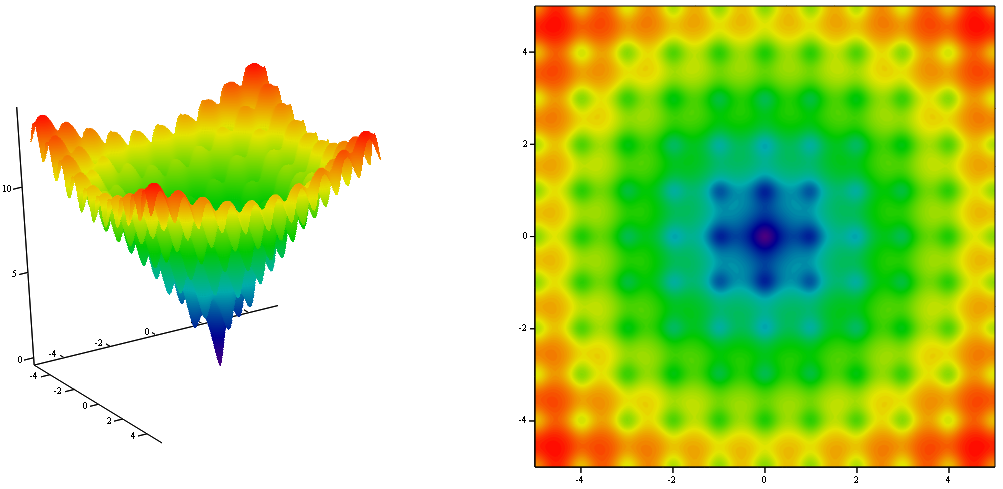
\includegraphics [scale=0.5] {MHL_TestFunction_Ackley}
  \caption{Функция Ackley} 
  \label{TestFunctions:img:MHL_TestFunction_Ackleye}  
\end{figure}

\subsection {Параметры для алгоритмов оптимизации}

\begin{tabularwide}
\textbf{Точность вычислений:} & $\varepsilon=0.025$. \\
\textbf{Число интервалов, на которые предполагается разбивать каждую компоненту вектора $\bar{x}$ в пределах своего изменения} (для алгоритмов дискретной оптимизации) : & $NumberOfParts_j=4095$ ($j=\overline{1,n}$). \\
\textbf{Для этого длина бинарной строки для $x_j$ координаты равна} (для алгоритмов бинарной оптимизации) : & $\left( k_2\right)_j=12$ ($j=\overline{1,n}$). \\
\end{tabularwide}

\textbf{Замечание:}  $NumberOfParts_j$ выбирается как минимальное число, удовлетворяющее соотношению:
\begin{equation*}
NumberOfParts_j=2^{\left( k_2\right)_j }-1\geq\dfrac{10\left( Right_j-Left_j\right) }{\varepsilon},\text{где } \left( k_2\right)_j \in \mathbb{N}, \left( j=\overline{1,n}\right).
\end{equation*}

\subsection {Основная задача и подзадачи}

\begin{tabularwide}
\textbf{Изменяемый параметр: } & $n$ --- размерность вещественного вектора. \\
\textbf{Значение в основной задаче:} & $n=2$.\\
\textbf{Подзадача №2:} & $n=3$.\\
\textbf{Подзадача №3:} & $n=4$.\\
\textbf{Подзадача №4:} & $n=5$.\\
\textbf{Подзадача №5:} & $n=10$.\\
\textbf{Подзадача №6:} & $n=20$.\\
\textbf{Подзадача №7:} & $n=30$.\\
\end{tabularwide}

\subsection {Нахождение ошибки оптимизации}

Пусть в результате работы алгоритма оптимизации за $N$ запусков мы нашли решения $\bar{x}_{submin}^k$ со значениями целевой функции $f\left( \bar{x}_{submin}^k\right) $ соответственно ($k=\overline{1,N}$). Используем три вида ошибок:

\textbf{Надёжность: }
\begin{equation*}
R = \dfrac{\sum_{k=1}^{N}S\left( \bar{x}_{submin}^k \right) }{N}, \text{ где}
\end{equation*}
\begin{equation*}
S\left( \bar{x}_{submin}^k \right)=\left\lbrace \begin{aligned} 1,& \text{ если } \left| \left( \bar{x}_{submin}^k \right)_j-\left( \bar{x}_{min} \right)_j\right|<\varepsilon, j=\overline{1,n};   \\ 0,& \text{ иначе}. \end{aligned}\right.
\end{equation*}

\textbf{Ошибка по входным параметрам:}
\begin{equation*}
E_x = \dfrac{\sum_{k=1}^{N} \left( \frac{\sqrt{\sum_{j=1}^{n}{\left( \left( \bar{x}_{submin}^k \right)_j-\left( \bar{x}_{min} \right)_j \right)}^2 }}{n} \right)  }{N}.
\end{equation*}

\textbf{Ошибка по значениям целевой функции: }
\begin{equation*}
E_f = \dfrac{\sum_{k=1}^{N} \left| f\left( \bar{x}_{submin}^k \right)-f\left( \bar{x}_{min} \right) \right|  }{N}.
\end{equation*}

\subsection {Свойства задачи}
\begin{tabularwide}
\textbf{Условной или безусловной оптимизации: } & Задача безусловной оптимизации. \\
\textbf{Одномерной или многомерной оптимизации: } & Многомерной: $ n $. \\
\textbf{Функция унимодальная или многоэкстремальная: } & Функция многоэкстремальная. \\
\textbf{Функция стохастическая или нет: } & Функция не стохастическая. \\
\textbf{Особенности: } & Нет. \\
\end{tabularwide}

\subsection {Реализация}

Реализация функции взята из библиотеки HarrixMathLibrary в разделе <<Тестовые функции для оптимизации>>, которую можно найти по адресу \href{https://github.com/Harrix/HarrixMathLibrary} {https://github.com/Harrix/HarrixMathLibrary}.

\begin{lstlisting}[caption=Код функции MHL\_TestFunction\_Ackley]
double MHL_TestFunction_Ackley(double *x, int VMHL_N)
{
/*
Функция многих переменных: Ackley.
Тестовая функция вещественной оптимизации.
Входные параметры:
 x - указатель на исходный массив;
 VMHL_N - размер массива x.
Возвращаемое значение:
 Значение тестовой функции в точке x.
*/
double VMHL_Result;
double f1,f2=0;
f1=exp(-0.2*sqrt(TMHL_SumSquareVector(x,VMHL_N)/double(VMHL_N)));
for (int i=0;i<VMHL_N;i++) f2=f2+cos(2.*MHL_PI*x[i]);
f2=exp(f2/double(VMHL_N));
VMHL_Result=20.+exp(1)-20.*f1-f2;
return VMHL_Result;
}
\end{lstlisting}

\subsection {Ссылки}

Данная функция приводится в следующих источниках:

\begin{enumerate}
\item \cite[стр. 5]{web:1207.4318} ---  \href{http://arxiv.org/pdf/1207.4318v1.pdf}{Empirical review of standard benchmark functions using evolutionary global optimization}.
\item \cite{web:www.cs.unm.edu:AckleysFunction} ---  \href{http://www.cs.unm.edu/~neal.holts/dga/benchmarkFunction/ackley.html}{Ackley's Function}.
\end{enumerate}
\section {Функция Гриванка}

\subsection {Описание функции}

\begin{tabularwide}
\textbf{Идентификатор:} & MHL\_TestFunction\_Griewangk. \\
\textbf{Наименование:} & Функция Гриванка. \\
\textbf{Тип:} & Задача вещественной оптимизации. \\
\end{tabularwide}

\textbf{Формула} (целевая функция):
\begin{equation}
\label{TestFunctions:eq:MHL_TestFunction_Griewangk}
f\left( \bar{x}\right) = \sum_{i=1}^{n}\dfrac{\bar{x}_i^2}{4000}-\prod_{i=1}^{n}\cos\left( \dfrac{\bar{x}_i}{\sqrt{i}}\right)+1 , \text{ где}
\end{equation}
\indent $\bar{x}\in X$, $\bar{x}_j\in \left[ Left_j; Right_j\right] $, $Left_j=-16$, $Right_j=16$, $j=\overline{1,n}$.

\begin{tabularwide}
\textbf{Обозначение:} &\specialcell{$\bar{x}$ --- вещественный вектор;\\$n$ --- размерность вещественного вектора.}  \\
\textbf{Решаемая задача оптимизации:} & $\bar{x}_{min}= \arg \min_{\bar{x}\in X} f\left( \bar{x}\right)$.   \\
\textbf{Точка минимума:} & $\bar{x}_{min}={\left( 0,0,\ldots,0\right)}^\mathrm{T} $, то есть $\left(\bar{x}_{min} \right)_j=0$ ($j=\overline{1,n}$).    \\
\textbf{Минимум функции:} & $f\left(\bar{x}_{min} \right) =0$.   \\
\textbf{График:} & Рисунок \ref{TestFunctions:img:MHL_TestFunction_Griewangke} нас \pageref{TestFunctions:img:MHL_TestFunction_Griewangke} стр.   \\
\end{tabularwide}

\begin{figure} [h] 
  \center
  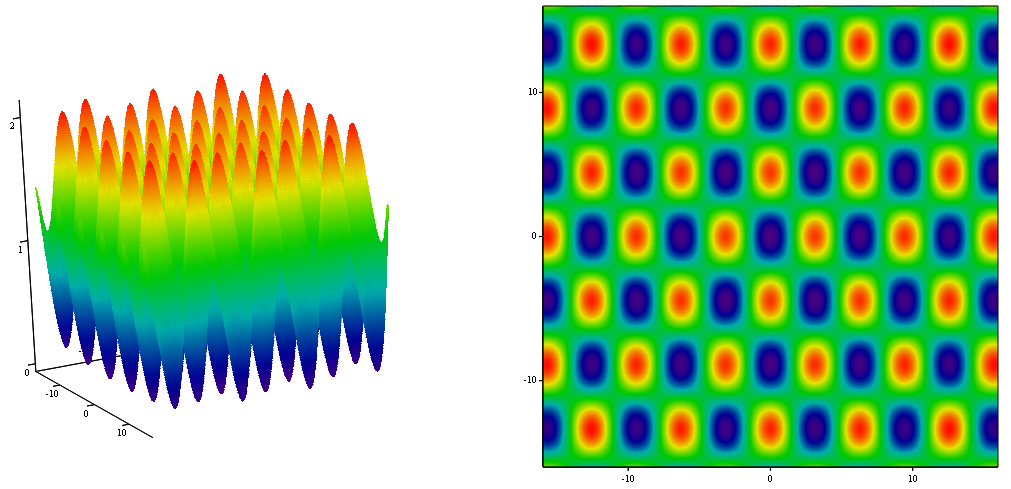
\includegraphics [scale=0.5] {MHL_TestFunction_Griewangk}
  \caption{Функция Гриванка} 
  \label{TestFunctions:img:MHL_TestFunction_Griewangke}  
\end{figure}

\subsection {Параметры для алгоритмов оптимизации}

\begin{tabularwide}
\textbf{Точность вычислений:} & $\varepsilon=0.08$. \\
\textbf{Число интервалов, на которые предполагается разбивать каждую компоненту вектора $\bar{x}$ в пределах своего изменения} (для алгоритмов дискретной оптимизации) : & $NumberOfParts_j=4095$ ($j=\overline{1,n}$). \\
\textbf{Для этого длина бинарной строки для $x_j$ координаты равна} (для алгоритмов бинарной оптимизации) : & $\left( k_2\right)_j=12$ ($j=\overline{1,n}$). \\
\end{tabularwide}

\textbf{Замечание:}  $NumberOfParts_j$ выбирается как минимальное число, удовлетворяющее соотношению:
\begin{equation*}
NumberOfParts_j=2^{\left( k_2\right)_j }-1\geq\dfrac{10\left( Right_j-Left_j\right) }{\varepsilon},\text{где } \left( k_2\right)_j \in \mathbb{N}, \left( j=\overline{1,n}\right).
\end{equation*}

\subsection {Основная задача и подзадачи}

\begin{tabularwide}
\textbf{Изменяемый параметр: } & $n$ --- размерность вещественного вектора. \\
\textbf{Значение в основной задаче:} & $n=2$.\\
\textbf{Подзадача №2:} & $n=3$.\\
\textbf{Подзадача №3:} & $n=4$.\\
\textbf{Подзадача №4:} & $n=5$.\\
\textbf{Подзадача №5:} & $n=10$.\\
\textbf{Подзадача №6:} & $n=20$.\\
\textbf{Подзадача №7:} & $n=30$.\\
\end{tabularwide}

\subsection {Нахождение ошибки оптимизации}

Пусть в результате работы алгоритма оптимизации за $N$ запусков мы нашли решения $\bar{x}_{submin}^k$ со значениями целевой функции $f\left( \bar{x}_{submin}^k\right) $ соответственно ($k=\overline{1,N}$). Используем три вида ошибок:

\textbf{Надёжность: }
\begin{equation*}
R = \dfrac{\sum_{k=1}^{N}S\left( \bar{x}_{submin}^k \right) }{N}, \text{ где}
\end{equation*}
\begin{equation*}
S\left( \bar{x}_{submin}^k \right)=\left\lbrace \begin{aligned} 1,& \text{ если } \left| \left( \bar{x}_{submin}^k \right)_j-\left( \bar{x}_{min} \right)_j\right|<\varepsilon, j=\overline{1,n};   \\ 0,& \text{ иначе}. \end{aligned}\right.
\end{equation*}

\textbf{Ошибка по входным параметрам:}
\begin{equation*}
E_x = \dfrac{\sum_{k=1}^{N} \left( \frac{\sqrt{\sum_{j=1}^{n}{\left( \left( \bar{x}_{submin}^k \right)_j-\left( \bar{x}_{min} \right)_j \right)}^2 }}{n} \right)  }{N}.
\end{equation*}

\textbf{Ошибка по значениям целевой функции: }
\begin{equation*}
E_f = \dfrac{\sum_{k=1}^{N} \left| f\left( \bar{x}_{submin}^k \right)-f\left( \bar{x}_{min} \right) \right|  }{N}.
\end{equation*}

\subsection {Свойства задачи}
\begin{tabularwide}
\textbf{Условной или безусловной оптимизации: } & Задача безусловной оптимизации. \\
\textbf{Одномерной или многомерной оптимизации: } & Многомерной: $ n $. \\
\textbf{Функция унимодальная или многоэкстремальная: } & Функция многоэкстремальная. \\
\textbf{Функция стохастическая или нет: } & Функция не стохастическая. \\
\textbf{Особенности: } & Локальные минимумы очень похожи на глобальный по своему значению. \\
\end{tabularwide}

\subsection {Реализация}

Реализация функции взята из библиотеки HarrixMathLibrary в разделе <<Тестовые функции для оптимизации>>, которую можно найти по адресу \href{https://github.com/Harrix/HarrixMathLibrary} {https://github.com/Harrix/HarrixMathLibrary}.

\begin{lstlisting}[caption=Код функции MHL\_TestFunction\_Griewangk]
double MHL_TestFunction_Griewangk(double *x, int VMHL_N)
{
/*
Функция многих переменных: функция Гриванка.
Тестовая функция вещественной оптимизации.
Входные параметры:
 x - указатель на исходный массив;
 VMHL_N - размер массива x.
Возвращаемое значение:
 Значение тестовой функции в точке x.
*/
double VMHL_Result=0;
double f=1;
int i;

for (i=0;i<VMHL_N;i++) VMHL_Result+=x[i]*x[i];
VMHL_Result/=4000.;

for (i=0;i<VMHL_N;i++) f=f*cos(x[i]/sqrt(i+1));

VMHL_Result=VMHL_Result-f+1.;

return VMHL_Result;
}
\end{lstlisting}

\subsection {Ссылки}

Данная функция приводится в следующих источниках:

\begin{enumerate}
\item \cite[стр. 7]{web:GEATbxExamples} ---  \href{http://www.geatbx.com/download/GEATbx_ObjFunExpl_v38.pdf}{GEATbx Examples. Examples of Objective Functions}.
\item \cite[стр. 16]{article:2013arXiv1308.4008J} ---  \href{http://arxiv.org/pdf/1308.4008.pdf}{A Literature Survey of Benchmark Functions For Global Optimization Problems}.
\end{enumerate}
\section {Функция Гипер-эллипсоид}

\subsection {Описание функции}

\begin{tabularwide}
\textbf{Идентификатор:} & MHL\_TestFunction\_HyperEllipsoid. \\
\textbf{Наименование:} & Гипер-эллипсоид. \\
\textbf{Тип:} & Задача вещественной оптимизации. \\
\end{tabularwide}

\textbf{Формула} (целевая функция):
\begin{equation}
\label{TestFunctions:eq:MHL_TestFunction_HyperEllipsoid}
f\left( \bar{x}\right) = \sum_{i=1}^{n}\left( i\cdot\bar{x}_i\right) ^2, \text{ где}
\end{equation}
\indent $\bar{x}\in X$, $\bar{x}_j\in \left[ Left_j; Right_j\right] $, $Left_j=-5$, $Right_j=5$, $j=\overline{1,n}$.

\begin{tabularwide}
\textbf{Обозначение:} &\specialcell{$\bar{x}$ --- вещественный вектор;\\$n$ --- размерность вещественного вектора.}  \\
\textbf{Решаемая задача оптимизации:} & $\bar{x}_{min}= \arg \min_{\bar{x}\in X} f\left( \bar{x}\right)$.   \\
\textbf{Точка минимума:} & $\bar{x}_{min}={\left( 0,0,\ldots,0\right)}^\mathrm{T} $, то есть $\left(\bar{x}_{min} \right)_j=0$ ($j=\overline{1,n}$).    \\
\textbf{Минимум функции:} & $f\left(\bar{x}_{min} \right) =0$.   \\
\textbf{График:} & Рисунок \ref{TestFunctions:img:MHL_TestFunction_HyperEllipsoide} нас \pageref{TestFunctions:img:MHL_TestFunction_HyperEllipsoide} стр.   \\
\end{tabularwide}

\begin{figure} [h] 
  \center
  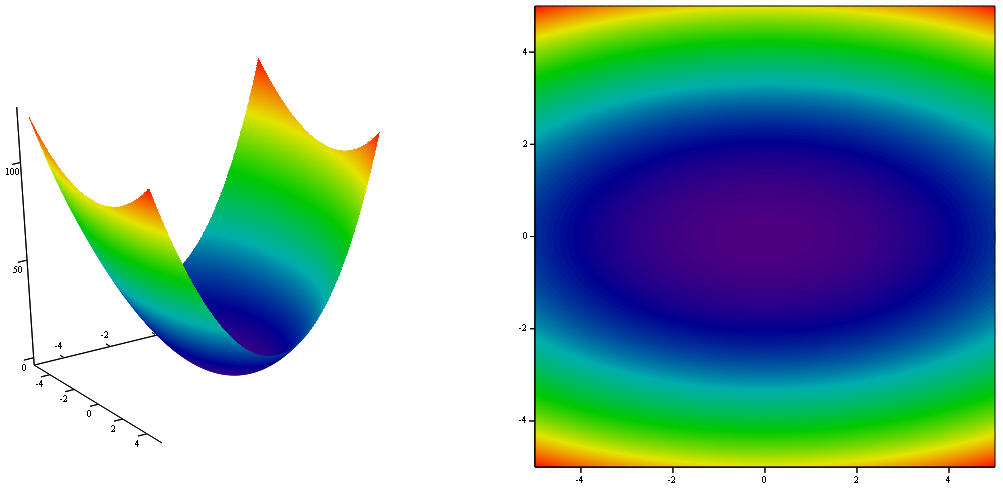
\includegraphics [scale=0.5] {MHL_TestFunction_HyperEllipsoid}
  \caption{Гипер-эллипсоид} 
  \label{TestFunctions:img:MHL_TestFunction_HyperEllipsoide}  
\end{figure}

\subsection {Параметры для алгоритмов оптимизации}

\begin{tabularwide}
\textbf{Точность вычислений:} & $\varepsilon=0.025$. \\
\textbf{Число интервалов, на которые предполагается разбивать каждую компоненту вектора $\bar{x}$ в пределах своего изменения} (для алгоритмов дискретной оптимизации) : & $NumberOfParts_j=4095$ ($j=\overline{1,n}$). \\
\textbf{Для этого длина бинарной строки для $x_j$ координаты равна} (для алгоритмов бинарной оптимизации) : & $\left( k_2\right)_j=12$ ($j=\overline{1,n}$). \\
\end{tabularwide}

\textbf{Замечание:}  $NumberOfParts_j$ выбирается как минимальное число, удовлетворяющее соотношению:
\begin{equation*}
NumberOfParts_j=2^{\left( k_2\right)_j }-1\geq\dfrac{10\left( Right_j-Left_j\right) }{\varepsilon},\text{где } \left( k_2\right)_j \in \mathbb{N}, \left( j=\overline{1,n}\right).
\end{equation*}

\subsection {Основная задача и подзадачи}

\begin{tabularwide}
\textbf{Изменяемый параметр: } & $n$ --- размерность вещественного вектора. \\
\textbf{Значение в основной задаче:} & $n=2$.\\
\textbf{Подзадача №2:} & $n=3$.\\
\textbf{Подзадача №3:} & $n=4$.\\
\textbf{Подзадача №4:} & $n=5$.\\
\textbf{Подзадача №5:} & $n=10$.\\
\textbf{Подзадача №6:} & $n=20$.\\
\textbf{Подзадача №7:} & $n=30$.\\
\end{tabularwide}

\subsection {Нахождение ошибки оптимизации}

Пусть в результате работы алгоритма оптимизации за $N$ запусков мы нашли решения $\bar{x}_{submin}^k$ со значениями целевой функции $f\left( \bar{x}_{submin}^k\right) $ соответственно ($k=\overline{1,N}$). Используем три вида ошибок:

\textbf{Надёжность: }
\begin{equation*}
R = \dfrac{\sum_{k=1}^{N}S\left( \bar{x}_{submin}^k \right) }{N}, \text{ где}
\end{equation*}
\begin{equation*}
S\left( \bar{x}_{submin}^k \right)=\left\lbrace \begin{aligned} 1,& \text{ если } \left| \left( \bar{x}_{submin}^k \right)_j-\left( \bar{x}_{min} \right)_j\right|\leq\varepsilon, j=\overline{1,n};   \\ 0,& \text{ иначе}. \end{aligned}\right.
\end{equation*}

\textbf{Ошибка по входным параметрам:}
\begin{equation*}
E_x = \dfrac{\sum_{k=1}^{N} \left( \frac{\sqrt{\sum_{j=1}^{n}{\left( \left( \bar{x}_{submin}^k \right)_j-\left( \bar{x}_{min} \right)_j \right)}^2 }}{n} \right)  }{N}.
\end{equation*}

\textbf{Ошибка по значениям целевой функции: }
\begin{equation*}
E_f = \dfrac{\sum_{k=1}^{N} \left| f\left( \bar{x}_{submin}^k \right)-f\left( \bar{x}_{min} \right) \right|  }{N}.
\end{equation*}

\subsection {Свойства задачи}
\begin{tabularwide}
\textbf{Условной или безусловной оптимизации: } & Задача безусловной оптимизации. \\
\textbf{Одномерной или многомерной оптимизации: } & Многомерной: $ n $. \\
\textbf{Функция унимодальная или многоэкстремальная: } & Функция унимодальная. \\
\textbf{Функция стохастическая или нет: } & Функция не стохастическая. \\
\textbf{Особенности: } & Нет. \\
\end{tabularwide}

\subsection {Реализация}

Реализация функции взята из библиотеки HarrixMathLibrary в разделе <<Тестовые функции для оптимизации>>, которую можно найти по адресу \href{https://github.com/Harrix/HarrixMathLibrary} {https://github.com/Harrix/HarrixMathLibrary}.

\begin{lstlisting}[caption=Код функции MHL\_TestFunction\_HyperEllipsoid]
double MHL_TestFunction_HyperEllipsoid(double *x, int VMHL_N)
{
/*
Функция многих переменных: Гипер-эллипсоид.
Тестовая функция вещественной оптимизации.
Входные параметры:
 x - указатель на исходный массив;
 VMHL_N - размер массива x.
Возвращаемое значение:
 Значение тестовой функции в точке x.
*/
double VMHL_Result=0;

for (int i=0;i<VMHL_N;i++)
	VMHL_Result += (i+1)*(i+1)*x[i]*x[i];

return VMHL_Result;
}
\end{lstlisting}

\subsection {Ссылки}

В данном виде тестовую функцию в литературе не нашел. Обычно используется несколько иной вид этой функции, когда $ i $ не возводится в квадрат.
\section {Эллиптический параболоид}

\subsection {Описание функции}

\begin{tabularwide}
\textbf{Идентификатор:} & MHL\_TestFunction\_ParaboloidOfRevolution. \\
\textbf{Наименование:} & Эллиптический параболоид. \\
\textbf{Тип:} & Задача вещественной оптимизации. \\
\end{tabularwide}

\textbf{Формула} (целевая функция):
\begin{equation}
\label{TestFunctions:eq:MHL_TestFunction_ParaboloidOfRevolution}
f\left( \bar{x}\right) = \sum_{i=1}^{n}\bar{x}_i^2, \text{ где}
\end{equation}
\indent $\bar{x}\in X$, $\bar{x}_j\in \left[ Left_j; Right_j\right] $, $Left_j=-2$, $Right_j=2$, $j=\overline{1,n}$.

\begin{tabularwide}
\textbf{Обозначение:} &\specialcell{$\bar{x}$ --- вещественный вектор;\\$n$ --- размерность вещественного вектора.}  \\
\textbf{Решаемая задача оптимизации:} & $\bar{x}_{min}= \arg \min_{\bar{x}\in X} f\left( \bar{x}\right)$.   \\
\textbf{Точка минимума:} & $\bar{x}_{min}={\left( 0,0,\ldots,0\right)}^\mathrm{T} $, то есть $\left(\bar{x}_{min} \right)_j=0$ ($j=\overline{1,n}$).    \\
\textbf{Минимум функции:} & $f\left(\bar{x}_{min} \right) =0$.   \\
\textbf{График:} & Рисунок \ref{TestFunctions:img:MHL_TestFunction_ParaboloidOfRevolution} нас \pageref{TestFunctions:img:MHL_TestFunction_ParaboloidOfRevolution} стр.   \\
\end{tabularwide}

\begin{figure} [h] 
  \center
  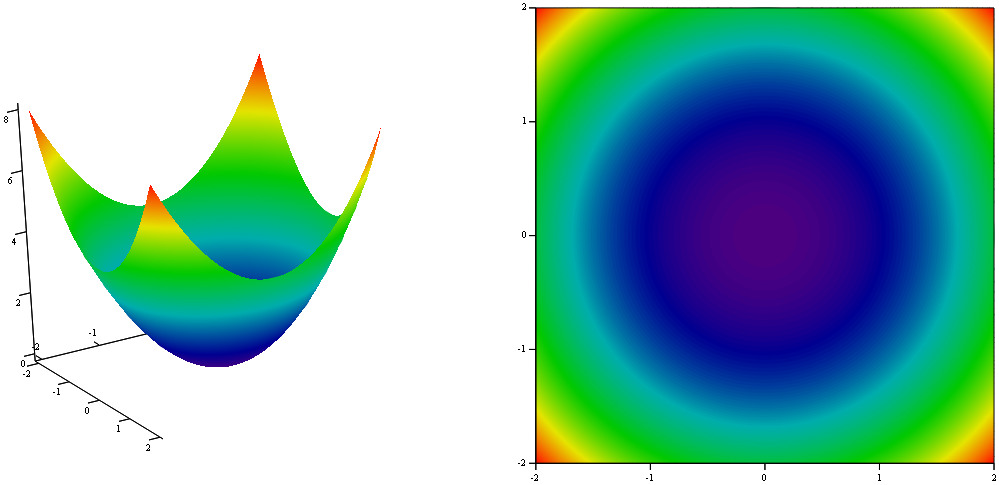
\includegraphics [scale=0.5] {MHL_TestFunction_ParaboloidOfRevolution}
  \caption{Эллиптический параболоид} 
  \label{TestFunctions:img:MHL_TestFunction_ParaboloidOfRevolution}  
\end{figure}

\subsection {Параметры для алгоритмов оптимизации}

\begin{tabularwide}
\textbf{Точность вычислений:} & $\varepsilon=0.01$. \\
\textbf{Число интервалов, на которые предполагается разбивать каждую компоненту вектора $\bar{x}$ в пределах своего изменения} (для алгоритмов дискретной оптимизации) : & $NumberOfParts_j=4095$ ($j=\overline{1,n}$). \\
\textbf{Для этого длина бинарной строки для $x_j$ координаты равна} (для алгоритмов бинарной оптимизации) : & $\left( k_2\right)_j=12$ ($j=\overline{1,n}$). \\
\end{tabularwide}

\textbf{Замечание:}  $NumberOfParts_j$ выбирается как минимальное число, удовлетворяющее соотношению:
\begin{equation*}
NumberOfParts_j=2^{\left( k_2\right)_j }-1\geq\dfrac{10\left( Right_j-Left_j\right) }{\varepsilon},\text{где } \left( k_2\right)_j \in \mathbb{N}, \left( j=\overline{1,n}\right).
\end{equation*}

\subsection {Основная задача и подзадачи}

\begin{tabularwide}
\textbf{Изменяемый параметр: } & $n$ --- размерность вещественного вектора. \\
\textbf{Значение в основной задаче:} & $n=2$.\\
\textbf{Подзадача №2:} & $n=3$.\\
\textbf{Подзадача №3:} & $n=4$.\\
\textbf{Подзадача №4:} & $n=5$.\\
\textbf{Подзадача №5:} & $n=10$.\\
\textbf{Подзадача №6:} & $n=20$.\\
\textbf{Подзадача №7:} & $n=30$.\\
\end{tabularwide}

\subsection {Нахождение ошибки оптимизации}

Пусть в результате работы алгоритма оптимизации за $N$ запусков мы нашли решения $\bar{x}_{submin}^k$ со значениями целевой функции $f\left( \bar{x}_{submin}^k\right) $ соответственно ($k=\overline{1,N}$). Используем три вида ошибок:

\textbf{Надёжность: }
\begin{equation*}
R = \dfrac{\sum_{k=1}^{N}S\left( \bar{x}_{submin}^k \right) }{N}, \text{ где}
\end{equation*}
\begin{equation*}
S\left( \bar{x}_{submin}^k \right)=\left\lbrace \begin{aligned} 1,& \text{ если } \left| \left( \bar{x}_{submin}^k \right)_j-\left( \bar{x}_{min} \right)_j\right|<\varepsilon, j=\overline{1,n};   \\ 0,& \text{ иначе}. \end{aligned}\right.
\end{equation*}

\textbf{Ошибка по входным параметрам:}
\begin{equation*}
E_x = \dfrac{\sum_{k=1}^{N} \left( \frac{\sqrt{\sum_{j=1}^{n}{\left( \left( \bar{x}_{submin}^k \right)_j-\left( \bar{x}_{min} \right)_j \right)}^2 }}{n} \right)  }{N}.
\end{equation*}

\textbf{Ошибка по значениям целевой функции: }
\begin{equation*}
E_f = \dfrac{\sum_{k=1}^{N} \left| f\left( \bar{x}_{submin}^k \right)-f\left( \bar{x}_{min} \right) \right|  }{N}.
\end{equation*}

\subsection {Свойства задачи}
\begin{tabularwide}
\textbf{Условной или безусловной оптимизации: } & Задача безусловной оптимизации. \\
\textbf{Одномерной или многомерной оптимизации: } & Многомерной: $ n $. \\
\textbf{Функция унимодальная или многоэкстремальная: } & Функция унимодальная. \\
\textbf{Функция стохастическая или нет: } & Функция не стохастическая. \\
\textbf{Особенности: } & Нет. \\
\end{tabularwide}

\subsection {Реализация}

Реализация функции взята из библиотеки HarrixMathLibrary в разделе <<Тестовые функции для оптимизации>>, которую можно найти по адресу \href{https://github.com/Harrix/HarrixMathLibrary} {https://github.com/Harrix/HarrixMathLibrary}.

\begin{lstlisting}[caption=Код функции MHL\_TestFunction\_ParaboloidOfRevolution]
double MHL_TestFunction_ParaboloidOfRevolution(double *x, int VMHL_N)
{
/*
Функция многих переменных: Эллиптический параболоид.
Тестовая функция вещественной оптимизации.
Входные параметры:
 x - указатель на исходный массив;
 VMHL_N - размер массива x.
Возвращаемое значение:
 Значение тестовой функции в точке x.
*/
double VMHL_Result=0;
for (int i=0;i<VMHL_N;i++) VMHL_Result+=x[i]*x[i];
return VMHL_Result;
}
\end{lstlisting}

\subsection {Ссылки}

Данная функция приводится в следующих источниках:

\begin{enumerate}
\item \cite{web:Paraboloid} ---  \href{http://en.wikipedia.org/wiki/Paraboloid}{Paraboloid}.
\end{enumerate}
\section {Функция Растригина}
\label{TestFunctions:section:MHL_TestFunction_Rastrigin}
\subsection {Описание функции}

\begin{tabularwide}
\textbf{Идентификатор:} & MHL\_TestFunction\_Rastrigin. \\
\textbf{Наименование:} & Функция Растригина. \\
\textbf{Тип:} & Задача вещественной оптимизации. \\
\end{tabularwide}

\textbf{Формула} (целевая функция):
\begin{equation}
\label{TestFunctions:eq:MHL_TestFunction_Rastrigin}
f\left( \bar{x}\right) = 10n+\sum_{i=1}^{n}\left( \bar{x}_i^2-10\cdot\cos\left( 2\pi\cdot \bar{x}_i\right) \right) , \text{ где}
\end{equation}
\indent $\bar{x}\in X$, $\bar{x}_j\in \left[ Left_j; Right_j\right] $, $Left_j=-5$, $Right_j=5$, $j=\overline{1,n}$.

\begin{tabularwide}
\textbf{Обозначение:} &\specialcell{$\bar{x}$ --- вещественный вектор;\\$n$ --- размерность вещественного вектора.}  \\
\textbf{Решаемая задача оптимизации:} & $\bar{x}_{min}= \arg \min_{\bar{x}\in X} f\left( \bar{x}\right)$.   \\
\textbf{Точка минимума:} & $\bar{x}_{min}={\left( 0,0,\ldots,0\right)}^\mathrm{T} $, то есть $\left(\bar{x}_{min} \right)_j=0$ ($j=\overline{1,n}$).    \\
\textbf{Минимум функции:} & $f\left(\bar{x}_{min} \right) =0$.   \\
\textbf{График:} & Рисунок \ref{TestFunctions:img:MHL_TestFunction_Rastrigin} нас \pageref{TestFunctions:img:MHL_TestFunction_Rastrigin} стр.   \\
\end{tabularwide}

\begin{figure} [h] 
  \center
  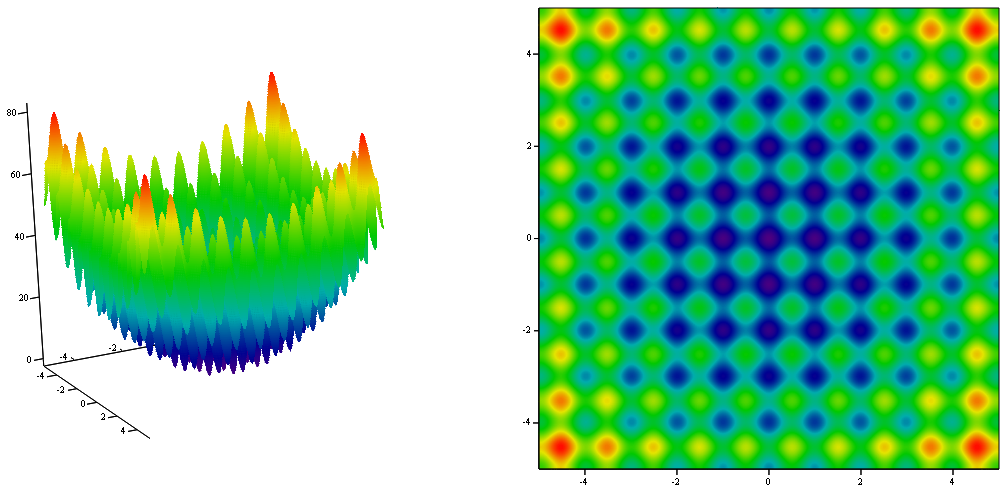
\includegraphics [scale=0.5] {MHL_TestFunction_Rastrigin}
  \caption{Функция Растригина} 
  \label{TestFunctions:img:MHL_TestFunction_Rastrigin}  
\end{figure}

\subsection {Параметры для алгоритмов оптимизации}

\begin{tabularwide}
\textbf{Точность вычислений:} & $\varepsilon=0.025$. \\
\textbf{Число интервалов, на которые предполагается разбивать каждую компоненту вектора $\bar{x}$ в пределах своего изменения} (для алгоритмов дискретной оптимизации) : & $NumberOfParts_j=4095$ ($j=\overline{1,n}$). \\
\textbf{Для этого длина бинарной строки для $x_j$ координаты равна} (для алгоритмов бинарной оптимизации) : & $\left( k_2\right)_j=12$ ($j=\overline{1,n}$). \\
\end{tabularwide}

\textbf{Замечание:}  $NumberOfParts_j$ выбирается как минимальное число, удовлетворяющее соотношению:
\begin{equation*}
NumberOfParts_j=2^{\left( k_2\right)_j }-1\geq\dfrac{10\left( Right_j-Left_j\right) }{\varepsilon},\text{где } \left( k_2\right)_j \in \mathbb{N}, \left( j=\overline{1,n}\right).
\end{equation*}

\subsection {Основная задача и подзадачи}

\begin{tabularwide}
\textbf{Изменяемый параметр: } & $n$ --- размерность вещественного вектора. \\
\textbf{Значение в основной задаче:} & $n=2$.\\
\textbf{Подзадача №2:} & $n=3$.\\
\textbf{Подзадача №3:} & $n=4$.\\
\textbf{Подзадача №4:} & $n=5$.\\
\textbf{Подзадача №5:} & $n=10$.\\
\textbf{Подзадача №6:} & $n=20$.\\
\textbf{Подзадача №7:} & $n=30$.\\
\end{tabularwide}

\subsection {Нахождение ошибки оптимизации}

Пусть в результате работы алгоритма оптимизации за $N$ запусков мы нашли решения $\bar{x}_{submin}^k$ со значениями целевой функции $f\left( \bar{x}_{submin}^k\right) $ соответственно ($k=\overline{1,N}$). Используем три вида ошибок:

\textbf{Надёжность: }
\begin{equation*}
R = \dfrac{\sum_{k=1}^{N}S\left( \bar{x}_{submin}^k \right) }{N}, \text{ где}
\end{equation*}
\begin{equation*}
S\left( \bar{x}_{submin}^k \right)=\left\lbrace \begin{aligned} 1,& \text{ если } \left| \left( \bar{x}_{submin}^k \right)_j-\left( \bar{x}_{min} \right)_j\right|<\varepsilon, j=\overline{1,n};   \\ 0,& \text{ иначе}. \end{aligned}\right.
\end{equation*}

\textbf{Ошибка по входным параметрам:}
\begin{equation*}
E_x = \dfrac{\sum_{k=1}^{N} \left( \frac{\sqrt{\sum_{j=1}^{n}{\left( \left( \bar{x}_{submin}^k \right)_j-\left( \bar{x}_{min} \right)_j \right)}^2 }}{n} \right)  }{N}.
\end{equation*}

\textbf{Ошибка по значениям целевой функции: }
\begin{equation*}
E_f = \dfrac{\sum_{k=1}^{N} \left| f\left( \bar{x}_{submin}^k \right)-f\left( \bar{x}_{min} \right) \right|  }{N}.
\end{equation*}

\subsection {Свойства задачи}
\begin{tabularwide}
\textbf{Условной или безусловной оптимизации: } & Задача безусловной оптимизации. \\
\textbf{Одномерной или многомерной оптимизации: } & Многомерной: $ n $. \\
\textbf{Функция унимодальная или многоэкстремальная: } & Функция многоэкстремальная. \\
\textbf{Функция стохастическая или нет: } & Функция не стохастическая. \\
\textbf{Особенности: } & Нет. \\
\end{tabularwide}

\subsection {Реализация}

Реализация функции взята из библиотеки HarrixMathLibrary в разделе <<Тестовые функции для оптимизации>>, которую можно найти по адресу \href{https://github.com/Harrix/HarrixMathLibrary} {https://github.com/Harrix/HarrixMathLibrary}.

\begin{lstlisting}[caption=Код функции MHL\_TestFunction\_Rastrigin]
double MHL_TestFunction_Rastrigin(double *x, int VMHL_N)
{
/*
Функция многих переменных: функция Растригина.
Тестовая функция вещественной оптимизации.
Входные параметры:
 x - указатель на исходный массив;
 VMHL_N - размер массива x.
Возвращаемое значение:
 Значение тестовой функции в точке x.
*/
double VMHL_Result=0;
for (int i=0;i<VMHL_N;i++) VMHL_Result+=x[i]*x[i]-10.*cos(2.*MHL_PI*x[i]);
VMHL_Result+=10*VMHL_N;
return VMHL_Result;
}
\end{lstlisting}

\subsection {Ссылки}

Данная функция приводится в следующих источниках:

\begin{enumerate}
\item \cite{web:wiki_Rastrigin_function} ---  \href{http://en.wikipedia.org/wiki/Rastrigin_function}{Rastrigin function}.
\item \cite{web:non_linear_continuous} ---  \href{http://www.maths.uq.edu.au/CEToolBox/node3.html}{Non-linear Continuous Multi-Extremal Optimization}.
\item \cite{web:parametric_optimization} ---  \href{http://www.pg.gda.pl/~mkwies/dyd/geadocu/fcnfun6.html}{Parametric Optimization}.
\end{enumerate}

\section {Функция Розенброка}
\label{TestFunctions:section:MHL_TestFunction_Rosenbrock}
\subsection {Описание функции}

\begin{tabularwide}
\textbf{Идентификатор:} & MHL\_TestFunction\_Rosenbrock. \\
\textbf{Наименование:} & Функция Розенброка. \\
\textbf{Тип:} & Задача вещественной оптимизации. \\
\end{tabularwide}

\textbf{Формула} (целевая функция):
\begin{equation}
\label{TestFunctions:eq:MHL_TestFunction_Rosenbrock}
f\left( \bar{x}\right) = \sum_{i=1}^{n-1} \left( 100{\left( \bar{x}_{i+1}-\bar{x}_i^2\right)}^2+{\left( 1-\bar{x}_i\right) }^2 \right)  , \text{ где}
\end{equation}
\indent $\bar{x}\in X$, $\bar{x}_j\in \left[ Left_j; Right_j\right] $, $Left_j=-2$, $Right_j=2$, $j=\overline{1,n}$.

\begin{tabularwide}
\textbf{Обозначение:} &\specialcell{$\bar{x}$ --- вещественный вектор;\\$n$ --- размерность вещественного вектора.}  \\
\textbf{Решаемая задача оптимизации:} & $\bar{x}_{min}= \arg \min_{\bar{x}\in X} f\left( \bar{x}\right)$.   \\
\textbf{Точка минимума:} & $\bar{x}_{min}={\left( 1,1,\ldots,1\right)}^\mathrm{T} $, то есть $\left(\bar{x}_{min} \right)_j=1$ ($j=\overline{1,n}$).    \\
\textbf{Минимум функции:} & $f\left(\bar{x}_{min} \right) =0$.   \\
\textbf{График:} & Рисунок \ref{TestFunctions:img:MHL_TestFunction_Rosenbrock} нас \pageref{TestFunctions:img:MHL_TestFunction_Rosenbrock} стр.   \\
\end{tabularwide}

\begin{figure} [h] 
  \center
  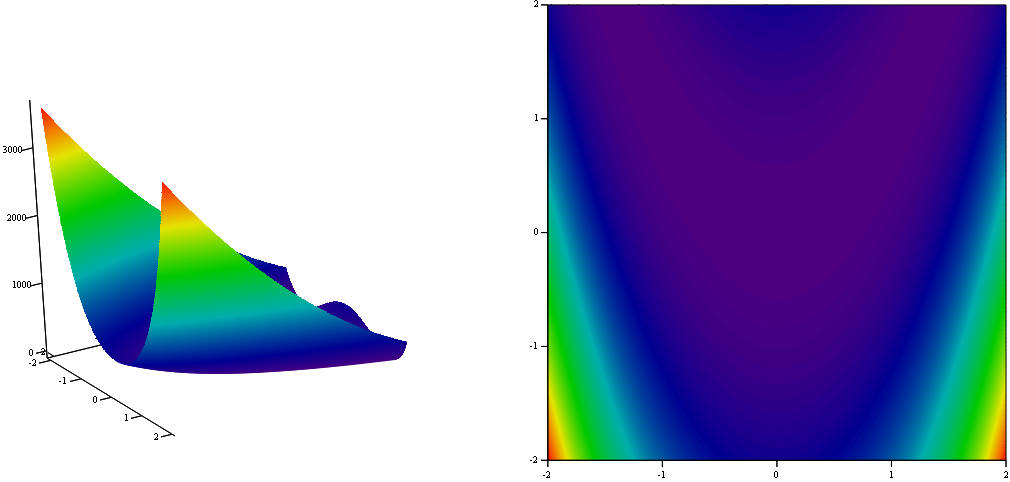
\includegraphics [scale=0.5] {MHL_TestFunction_Rosenbrock}
  \caption{Функция Розенброка} 
  \label{TestFunctions:img:MHL_TestFunction_Rosenbrock}  
\end{figure}

\subsection {Параметры для алгоритмов оптимизации}

\begin{tabularwide}
\textbf{Точность вычислений:} & $\varepsilon=0.01$. \\
\textbf{Число интервалов, на которые предполагается разбивать каждую компоненту вектора $\bar{x}$ в пределах своего изменения} (для алгоритмов дискретной оптимизации) : & $NumberOfParts_j=4095$ ($j=\overline{1,n}$). \\
\textbf{Для этого длина бинарной строки для $x_j$ координаты равна} (для алгоритмов бинарной оптимизации) : & $\left( k_2\right)_j=12$ ($j=\overline{1,n}$). \\
\end{tabularwide}

\textbf{Замечание:}  $NumberOfParts_j$ выбирается как минимальное число, удовлетворяющее соотношению:
\begin{equation*}
NumberOfParts_j=2^{\left( k_2\right)_j }-1\geq\dfrac{10\left( Right_j-Left_j\right) }{\varepsilon},\text{где } \left( k_2\right)_j \in \mathbb{N}, \left( j=\overline{1,n}\right).
\end{equation*}

\subsection {Основная задача и подзадачи}

\begin{tabularwide}
\textbf{Изменяемый параметр: } & $n$ --- размерность вещественного вектора. \\
\textbf{Значение в основной задаче:} & $n=2$.\\
\textbf{Подзадача №2:} & $n=3$.\\
\textbf{Подзадача №3:} & $n=4$.\\
\textbf{Подзадача №4:} & $n=5$.\\
\textbf{Подзадача №5:} & $n=10$.\\
\textbf{Подзадача №6:} & $n=20$.\\
\textbf{Подзадача №7:} & $n=30$.\\
\end{tabularwide}

\subsection {Нахождение ошибки оптимизации}

Пусть в результате работы алгоритма оптимизации за $N$ запусков мы нашли решения $\bar{x}_{submin}^k$ со значениями целевой функции $f\left( \bar{x}_{submin}^k\right) $ соответственно ($k=\overline{1,N}$). Используем три вида ошибок:

\textbf{Надёжность: }
\begin{equation*}
R = \dfrac{\sum_{k=1}^{N}S\left( \bar{x}_{submin}^k \right) }{N}, \text{ где}
\end{equation*}
\begin{equation*}
S\left( \bar{x}_{submin}^k \right)=\left\lbrace \begin{aligned} 1,& \text{ если } \left| \left( \bar{x}_{submin}^k \right)_j-\left( \bar{x}_{min} \right)_j\right|<\varepsilon, j=\overline{1,n};   \\ 0,& \text{ иначе}. \end{aligned}\right.
\end{equation*}

\textbf{Ошибка по входным параметрам:}
\begin{equation*}
E_x = \dfrac{\sum_{k=1}^{N} \left( \frac{\sqrt{\sum_{j=1}^{n}{\left( \left( \bar{x}_{submin}^k \right)_j-\left( \bar{x}_{min} \right)_j \right)}^2 }}{n} \right)  }{N}.
\end{equation*}

\textbf{Ошибка по значениям целевой функции: }
\begin{equation*}
E_f = \dfrac{\sum_{k=1}^{N} \left| f\left( \bar{x}_{submin}^k \right)-f\left( \bar{x}_{min} \right) \right|  }{N}.
\end{equation*}

\subsection {Свойства задачи}
\begin{tabularwide}
\textbf{Условной или безусловной оптимизации: } & Задача безусловной оптимизации. \\
\textbf{Одномерной или многомерной оптимизации: } & Многомерной: $ n $. \\
\textbf{Функция унимодальная или многоэкстремальная: } & Функция многоэкстремальная. \\
\textbf{Функция стохастическая или нет: } & Функция не стохастическая. \\
\textbf{Особенности: } & Нет. \\
\end{tabularwide}

\subsection {Реализация}

Реализация функции взята из библиотеки HarrixMathLibrary в разделе <<Тестовые функции для оптимизации>>, которую можно найти по адресу \href{https://github.com/Harrix/HarrixMathLibrary} {https://github.com/Harrix/HarrixMathLibrary}.

\begin{lstlisting}[caption=Код функции MHL\_TestFunction\_Rosenbrock]
double MHL_TestFunction_Rosenbrock(double *x, int VMHL_N)
{
/*
Функция многих переменных: функция Розенброка.
Тестовая функция вещественной оптимизации.
Входные параметры:
 x - указатель на исходный массив;
 VMHL_N - размер массива x.
Возвращаемое значение:
 Значение тестовой функции в точке x.
*/
double VMHL_Result=0;
for (int i=0;i<VMHL_N-1;i++) VMHL_Result+=100.*(x[i+1]-x[i]*x[i])*(x[i+1]-x[i]*x[i])+(1.-x[i])*(1.-x[i]);
return VMHL_Result;
}
\end{lstlisting}

\subsection {Ссылки}

Данная функция приводится в следующих источниках:

\begin{enumerate}
\item \cite{web:wiki_Rosenbrock_function} ---  \href{http://en.wikipedia.org/wiki/Rosenbrock_function}{Rosenbrock function}.
\item \cite{web:Rosenbrock_Function} ---  \href{http://www-optima.amp.i.kyoto-u.ac.jp/member/student/hedar/Hedar_files/TestGO_files/Page2537.htm}{Rosenbrock Function}.
\end{enumerate}
\section {Развернутый гипер-эллипсоид}

\subsection {Описание функции}

\begin{tabularwide}
\textbf{Идентификатор:} & MHL\_TestFunction\_RotatedHyperEllipsoid. \\
\textbf{Наименование:} & Развернутый гипер-эллипсоид. \\
\textbf{Тип:} & Задача вещественной оптимизации. \\
\end{tabularwide}

\textbf{Формула} (целевая функция):
\begin{equation}
\label{TestFunctions:eq:MHL_RotatedHyperEllipsoid}
f\left( \bar{x}\right) = \sum_{i=1}^{n}\left( \sum_{j=1}^{j}\bar{x}_j\right) ^2, \text{ где}
\end{equation}
\indent $\bar{x}\in X$, $\bar{x}_j\in \left[ Left_j; Right_j\right] $, $Left_j=-5$, $Right_j=5$, $j=\overline{1,n}$.

\begin{tabularwide}
\textbf{Обозначение:} &\specialcell{$\bar{x}$ --- вещественный вектор;\\$n$ --- размерность вещественного вектора.}  \\
\textbf{Решаемая задача оптимизации:} & $\bar{x}_{min}= \arg \min_{\bar{x}\in X} f\left( \bar{x}\right)$.   \\
\textbf{Точка минимума:} & $\bar{x}_{min}={\left( 0,0,\ldots,0\right)}^\mathrm{T} $, то есть $\left(\bar{x}_{min} \right)_j=0$ ($j=\overline{1,n}$).    \\
\textbf{Минимум функции:} & $f\left(\bar{x}_{min} \right) =0$.   \\
\textbf{График:} & Рисунок \ref{TestFunctions:img:MHL_TestFunction_RotatedHyperEllipsoide} нас \pageref{TestFunctions:img:MHL_TestFunction_RotatedHyperEllipsoide} стр.   \\
\end{tabularwide}

\begin{figure} [h] 
  \center
  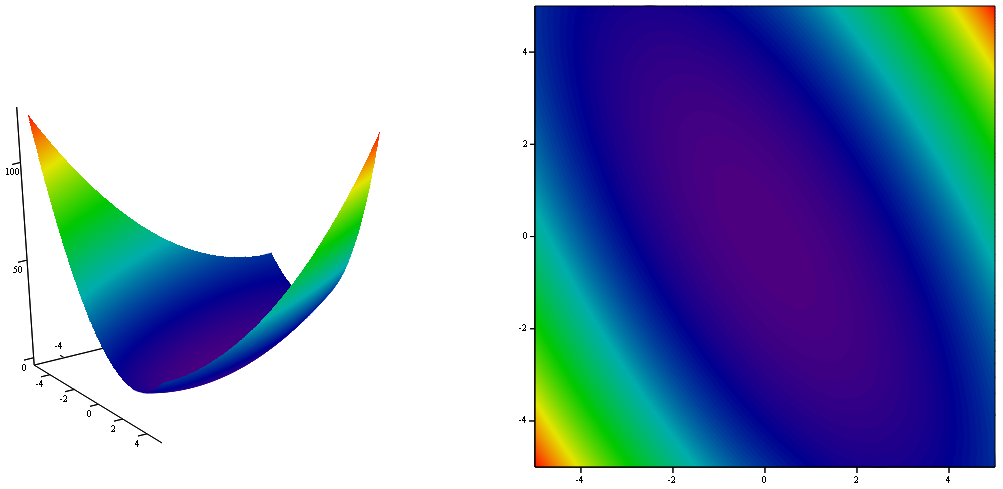
\includegraphics [scale=0.5] {MHL_TestFunction_RotatedHyperEllipsoid}
  \caption{Развернутый гипер-эллипсоид} 
  \label{TestFunctions:img:MHL_TestFunction_RotatedHyperEllipsoide}  
\end{figure}

\subsection {Параметры для алгоритмов оптимизации}

\begin{tabularwide}
\textbf{Точность вычислений:} & $\varepsilon=0.025$. \\
\textbf{Число интервалов, на которые предполагается разбивать каждую компоненту вектора $\bar{x}$ в пределах своего изменения} (для алгоритмов дискретной оптимизации) : & $NumberOfParts_j=4095$ ($j=\overline{1,n}$). \\
\textbf{Для этого длина бинарной строки для $x_j$ координаты равна} (для алгоритмов бинарной оптимизации) : & $\left( k_2\right)_j=12$ ($j=\overline{1,n}$). \\
\end{tabularwide}

\textbf{Замечание:}  $NumberOfParts_j$ выбирается как минимальное число, удовлетворяющее соотношению:
\begin{equation*}
NumberOfParts_j=2^{\left( k_2\right)_j }-1\geq\dfrac{10\left( Right_j-Left_j\right) }{\varepsilon},\text{где } \left( k_2\right)_j \in \mathbb{N}, \left( j=\overline{1,n}\right).
\end{equation*}

\subsection {Основная задача и подзадачи}

\begin{tabularwide}
\textbf{Изменяемый параметр: } & $n$ --- размерность вещественного вектора. \\
\textbf{Значение в основной задаче:} & $n=2$.\\
\textbf{Подзадача №2:} & $n=3$.\\
\textbf{Подзадача №3:} & $n=4$.\\
\textbf{Подзадача №4:} & $n=5$.\\
\textbf{Подзадача №5:} & $n=10$.\\
\textbf{Подзадача №6:} & $n=20$.\\
\textbf{Подзадача №7:} & $n=30$.\\
\end{tabularwide}

\subsection {Нахождение ошибки оптимизации}

Пусть в результате работы алгоритма оптимизации за $N$ запусков мы нашли решения $\bar{x}_{submin}^k$ со значениями целевой функции $f\left( \bar{x}_{submin}^k\right) $ соответственно ($k=\overline{1,N}$). Используем три вида ошибок:

\textbf{Надёжность: }
\begin{equation*}
R = \dfrac{\sum_{k=1}^{N}S\left( \bar{x}_{submin}^k \right) }{N}, \text{ где}
\end{equation*}
\begin{equation*}
S\left( \bar{x}_{submin}^k \right)=\left\lbrace \begin{aligned} 1,& \text{ если } \left| \left( \bar{x}_{submin}^k \right)_j-\left( \bar{x}_{min} \right)_j\right|<\varepsilon, j=\overline{1,n};   \\ 0,& \text{ иначе}. \end{aligned}\right.
\end{equation*}

\textbf{Ошибка по входным параметрам:}
\begin{equation*}
E_x = \dfrac{\sum_{k=1}^{N} \left( \frac{\sqrt{\sum_{j=1}^{n}{\left( \left( \bar{x}_{submin}^k \right)_j-\left( \bar{x}_{min} \right)_j \right)}^2 }}{n} \right)  }{N}.
\end{equation*}

\textbf{Ошибка по значениям целевой функции: }
\begin{equation*}
E_f = \dfrac{\sum_{k=1}^{N} \left| f\left( \bar{x}_{submin}^k \right)-f\left( \bar{x}_{min} \right) \right|  }{N}.
\end{equation*}

\subsection {Свойства задачи}
\begin{tabularwide}
\textbf{Условной или безусловной оптимизации: } & Задача безусловной оптимизации. \\
\textbf{Одномерной или многомерной оптимизации: } & Многомерной: $ n $. \\
\textbf{Функция унимодальная или многоэкстремальная: } & Функция унимодальная. \\
\textbf{Функция стохастическая или нет: } & Функция не стохастическая. \\
\textbf{Особенности: } & Нет. \\
\end{tabularwide}

\subsection {Реализация}

Реализация функции взята из библиотеки HarrixMathLibrary в разделе <<Тестовые функции для оптимизации>>, которую можно найти по адресу \href{https://github.com/Harrix/HarrixMathLibrary} {https://github.com/Harrix/HarrixMathLibrary}.

\begin{lstlisting}[caption=Код функции MHL\_TestFunction\_RotatedHyperEllipsoid]
double MHL_TestFunction_RotatedHyperEllipsoid(double *x, int VMHL_N)
{
/*
Функция многих переменных: Развернутый гипер-эллипсоид.
Тестовая функция вещественной оптимизации.
Входные параметры:
 x - указатель на исходный массив;
 VMHL_N - размер массива x.
Возвращаемое значение:
 Значение тестовой функции в точке x.
*/
double VMHL_Result=0;
double f;

for (int i=0;i<VMHL_N;i++)
 {
 f=0;
 for (int j=0;j<i+1;j++)
    f += x[j];
 VMHL_Result += f*f;
 }

return VMHL_Result;
}
\end{lstlisting}

\subsection {Ссылки}

Данная функция приводится в следующих источниках:

\begin{enumerate}
\item \cite[стр. 4]{web:GEATbxExamples} ---  \href{http://www.geatbx.com/download/GEATbx_ObjFunExpl_v38.pdf}{GEATbx Examples. Examples of Objective Functions}.
\end{enumerate}

Обратите внимание, что иногда под названием Rotated Hyper Ellipsoid встречается (например, \cite{web:www.sfu.ca:rotated_hyper-ellipsoid}) неправильно записанная функция в виде:
\begin{equation*}
\label{TestFunctions:eq:MHL_RotatedHyperEllipsoidError}
f\left( \bar{x}\right) = \sum_{i=1}^{n} \sum_{j=1}^{j}\bar{x}_j^2, \text{ где}
\end{equation*}

Данная функция не является развернутой по своему внешнему виду, поэтому автор склонен считать эту реализацию ошибочной.
\section {Функция Швефеля}
\label{TestFunctions:section:MHL_TestFunction_Schwefel}
\subsection {Описание функции}

\begin{tabularwide}
\textbf{Идентификатор:} & MHL\_TestFunction\_Schwefel. \\
\textbf{Наименование:} & Функция Швефеля. \\
\textbf{Тип:} & Задача вещественной оптимизации. \\
\end{tabularwide}

\textbf{Формула} (целевая функция):
\begin{equation}
\label{TestFunctions:eq:MHL_TestFunction_Schwefel}
f\left( \bar{x}\right) = 418.9829 n-\sum_{i=1}^{n}\left( \bar{x}_i\sin\left( \sqrt{\left| \bar{x}_i\right|}\right)  \right), \text{ где}
\end{equation}
\indent $\bar{x}\in X$, $\bar{x}_j\in \left[ Left_j; Right_j\right] $, $Left_j=-500$, $Right_j=500$, $j=\overline{1,n}$.

\begin{tabularwide}
\textbf{Обозначение:} &\specialcell{$\bar{x}$ --- вещественный вектор;\\$n$ --- размерность вещественного вектора.}  \\
\textbf{Решаемая задача оптимизации:} & $\bar{x}_{min}= \arg \min_{\bar{x}\in X} f\left( \bar{x}\right)$.   \\
\textbf{Точка минимума:} & $\bar{x}_{min}={\left( 420.968746,420.968746,\ldots,420.968746\right)}^\mathrm{T} $, то есть $\left(\bar{x}_{min} \right)_j=420.968746$ ($j=\overline{1,n}$).    \\
\textbf{Минимум функции:} & \specialcell{$f\left(\bar{x}_{min} \right) =0.0000255$, если $ n=2 $.\\$f\left(\bar{x}_{min} \right) =0.000127276$, если $ n=10$. \\То есть для каждого значения $ n$ надо пересчитывать\\ значение глобального минимума.}   \\
\textbf{График:} & Рисунок \ref{TestFunctions:img:MHL_TestFunction_Schwefele} нас \pageref{TestFunctions:img:MHL_TestFunction_Schwefele} стр.   \\
\end{tabularwide}

\begin{figure} [h] 
  \center
  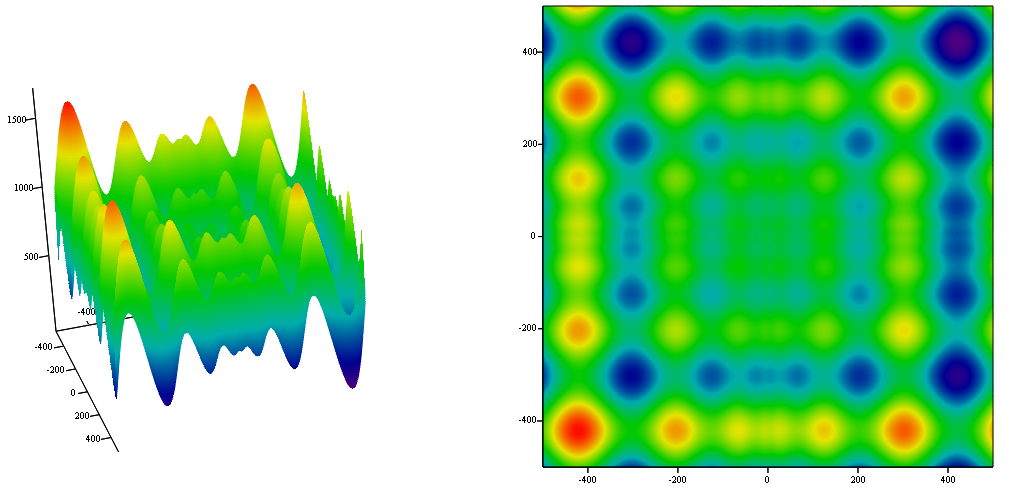
\includegraphics [scale=0.5] {MHL_TestFunction_Schwefel}
  \caption{Функция Швефеля} 
  \label{TestFunctions:img:MHL_TestFunction_Schwefele}  
\end{figure}

\subsection {Параметры для алгоритмов оптимизации}

\begin{tabularwide}
\textbf{Точность вычислений:} & $\varepsilon=2.5$. \\
\textbf{Число интервалов, на которые предполагается разбивать каждую компоненту вектора $\bar{x}$ в пределах своего изменения} (для алгоритмов дискретной оптимизации) : & $NumberOfParts_j=4095$ ($j=\overline{1,n}$). \\
\textbf{Для этого длина бинарной строки для $x_j$ координаты равна} (для алгоритмов бинарной оптимизации) : & $\left( k_2\right)_j=12$ ($j=\overline{1,n}$). \\
\end{tabularwide}

\textbf{Замечание:}  $NumberOfParts_j$ выбирается как минимальное число, удовлетворяющее соотношению:
\begin{equation*}
NumberOfParts_j=2^{\left( k_2\right)_j }-1\geq\dfrac{10\left( Right_j-Left_j\right) }{\varepsilon},\text{где } \left( k_2\right)_j \in \mathbb{N}, \left( j=\overline{1,n}\right).
\end{equation*}

\subsection {Основная задача и подзадачи}

\begin{tabularwide}
\textbf{Изменяемый параметр: } & $n$ --- размерность вещественного вектора. \\
\textbf{Значение в основной задаче:} & $n=2$.\\
\textbf{Подзадача №2:} & $n=3$.\\
\textbf{Подзадача №3:} & $n=4$.\\
\textbf{Подзадача №4:} & $n=5$.\\
\textbf{Подзадача №5:} & $n=10$.\\
\textbf{Подзадача №6:} & $n=20$.\\
\textbf{Подзадача №7:} & $n=30$.\\
\end{tabularwide}

\subsection {Нахождение ошибки оптимизации}

Пусть в результате работы алгоритма оптимизации за $N$ запусков мы нашли решения $\bar{x}_{submin}^k$ со значениями целевой функции $f\left( \bar{x}_{submin}^k\right) $ соответственно ($k=\overline{1,N}$). Используем три вида ошибок:

\textbf{Надёжность: }
\begin{equation*}
R = \dfrac{\sum_{k=1}^{N}S\left( \bar{x}_{submin}^k \right) }{N}, \text{ где}
\end{equation*}
\begin{equation*}
S\left( \bar{x}_{submin}^k \right)=\left\lbrace \begin{aligned} 1,& \text{ если } \left| \left( \bar{x}_{submin}^k \right)_j-\left( \bar{x}_{min} \right)_j\right|<\varepsilon, j=\overline{1,n};   \\ 0,& \text{ иначе}. \end{aligned}\right.
\end{equation*}

\textbf{Ошибка по входным параметрам:}
\begin{equation*}
E_x = \dfrac{\sum_{k=1}^{N} \left( \frac{\sqrt{\sum_{j=1}^{n}{\left( \left( \bar{x}_{submin}^k \right)_j-\left( \bar{x}_{min} \right)_j \right)}^2 }}{n} \right)  }{N}.
\end{equation*}

\textbf{Ошибка по значениям целевой функции: }
\begin{equation*}
E_f = \dfrac{\sum_{k=1}^{N} \left| f\left( \bar{x}_{submin}^k \right)-f\left( \bar{x}_{min} \right) \right|  }{N}.
\end{equation*}

\subsection {Свойства задачи}
\begin{tabularwide}
\textbf{Условной или безусловной оптимизации: } & Задача безусловной оптимизации. \\
\textbf{Одномерной или многомерной оптимизации: } & Многомерной: $ n $. \\
\textbf{Функция унимодальная или многоэкстремальная: } & Функция многоэкстремальная. \\
\textbf{Функция стохастическая или нет: } & Функция не стохастическая. \\
\textbf{Особенности: } & Для каждого значения $ n$ надо пересчитывать значение глобального минимума. \\
\end{tabularwide}

\subsection {Реализация}

Реализация функции взята из библиотеки HarrixMathLibrary в разделе <<Тестовые функции для оптимизации>>, которую можно найти по адресу \href{https://github.com/Harrix/HarrixMathLibrary} {https://github.com/Harrix/HarrixMathLibrary}.

\begin{lstlisting}[caption=Код функции MHL\_TestFunction\_Schwefel]
double double MHL_TestFunction_Schwefel(double *x, int VMHL_N)
{
/*
Функция многих переменных: функция Швефеля.
Тестовая функция вещественной оптимизации.
Входные параметры:
 x - указатель на исходный массив;
 VMHL_N - размер массива x.
Возвращаемое значение:
 Значение тестовой функции в точке x.
*/
double VMHL_Result=418.9829*VMHL_N;

for (int i=0;i<VMHL_N;i++)
    VMHL_Result -= x[i]*sin(sqrt(fabs(x[i])));

return VMHL_Result;
}
\end{lstlisting}

\subsection {Ссылки}

Данная функция приводится в следующих источниках:

\begin{enumerate}
\item \cite[стр. 9]{web:1207.4318} ---  \href{http://arxiv.org/pdf/1207.4318v1.pdf}{Empirical review of standard benchmark functions using evolutionary global optimization}.
\item \cite{web:www.cs.cmu.edu:BenchmarkProblems} ---  \href{http://www.cs.cmu.edu/afs/cs/project/jair/pub/volume24/ortizboyer05a-html/node6.html}{Benchmark Problems}.
\end{enumerate}

Обратите внимание, что в англоязычном секторе часто данная функция дается с обозначением глобального минимума в точке $\left(\bar{x}_{min} \right)_j=1$ ($j=\overline{1,n}$), $f\left(\bar{x}_{min} \right) =0$ (например, \cite{web:www.sfu.ca:SchwefelFunction}, \cite{web:www-optima.amp.i.kyoto-u.ac.jp:SchwefelFunction}). Это не правильно: $f\left(\begin{matrix}
1 \\ 1
\end{matrix} \right) =836.28286$. Скорее всего в каком-то источнике вначале допустили ошибку, и она стала копироваться в остальные.

В некоторых источниках (например, \cite{web:www.pg.gda.pl:Schwefelsfunction7}, \cite[стр. 7]{web:GEATbxExamples}) в формуле тестовой функции присутствует только второе слагаемое, а глобальный минимум определяется как $ 418.9829 n $. Это неправильно, так как хоть два слагаемых похожи друг на друга (\ref{TestFunctions:eq:MHL_TestFunction_Schwefel}), но они не дают строгий ноль в сумме, и при увеличении размерности различие между ними увеличивается.
\section {Функция Step (модифицированная версия De Jong 3)}

\subsection {Описание функции}

\begin{tabularwide}
\textbf{Идентификатор:} & MHL\_TestFunction\_StepFunction. \\
\textbf{Наименование:} & Функция Step (модифицированная версия De Jong 3). \\
\textbf{Тип:} & Задача вещественной оптимизации. \\
\end{tabularwide}

\textbf{Формула} (целевая функция):
\begin{equation}
\label{TestFunctions:eq:MHL_TestFunction_StepFunction}
f\left( \bar{x}\right) =\left\lbrace \begin{aligned}
\sum_{i=1}^{n} \left( int\left( \bar{x}_{i}\right)  \right)^2,& \text{ если} \sum_{i=1}^{n} \left| int\left( \bar{x}_{i}\right)\right| \neq 0 ;\\ \left( \sum_{i=1}^{n} \left| \bar{x}_{i}\right|\right) -1 ,& \text{ иначе}.
\end{aligned}\right. , \text{ где}
\end{equation}
\indent $\bar{x}\in X$, $\bar{x}_j\in \left[ Left_j; Right_j\right] $, $Left_j=-5$, $Right_j=5$, $j=\overline{1,n}$.

\begin{tabularwide}
\textbf{Обозначение:} &\specialcell{$\bar{x}$ --- вещественный вектор;\\$n$ --- размерность вещественного вектора.}  \\
\textbf{Решаемая задача оптимизации:} & $\bar{x}_{min}= \arg \min_{\bar{x}\in X} f\left( \bar{x}\right)$.   \\
\textbf{Точка минимума:} & $\bar{x}_{min}={\left( 0,0,\ldots,0\right)}^\mathrm{T} $, то есть $\left(\bar{x}_{min} \right)_j=0$ ($j=\overline{1,n}$).    \\
\textbf{Минимум функции:} & $f\left(\bar{x}_{min} \right) =-1$.   \\
\textbf{График:} & Рисунок \ref{TestFunctions:img:MHL_TestFunction_StepFunction} нас \pageref{TestFunctions:img:MHL_TestFunction_StepFunction} стр., \ref{TestFunctions:img:MHL_TestFunction_StepFunction_2img} нас \pageref{TestFunctions:img:MHL_TestFunction_StepFunction_2img} стр.  \\
\end{tabularwide}

\begin{figure} [h] 
  \center
  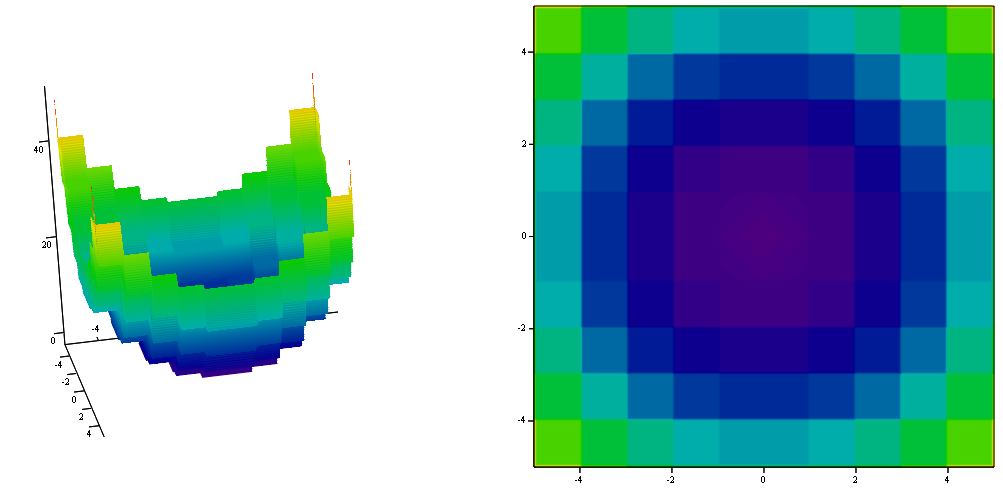
\includegraphics [scale=0.5] {MHL_TestFunction_StepFunction}
  \caption{Функция Step (модифицированная версия De Jong 3)} 
  \label{TestFunctions:img:MHL_TestFunction_StepFunction}  
\end{figure}

\begin{figure} [h] 
  \center
  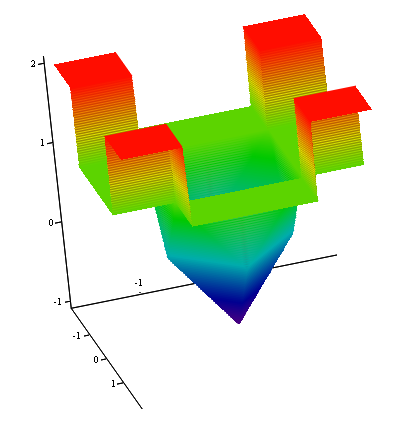
\includegraphics [scale=0.5] {MHL_TestFunction_StepFunction_2img}
  \caption{Функция Step (модифицированная версия De Jong 3) в области около точки минимума} 
  \label{TestFunctions:img:MHL_TestFunction_StepFunction_2img}  
\end{figure}

\subsection {Параметры для алгоритмов оптимизации}

\begin{tabularwide}
\textbf{Точность вычислений:} & $\varepsilon=0.025$. \\
\textbf{Число интервалов, на которые предполагается разбивать каждую компоненту вектора $\bar{x}$ в пределах своего изменения} (для алгоритмов дискретной оптимизации) : & $NumberOfParts_j=4095$ ($j=\overline{1,n}$). \\
\textbf{Для этого длина бинарной строки для $x_j$ координаты равна} (для алгоритмов бинарной оптимизации) : & $\left( k_2\right)_j=12$ ($j=\overline{1,n}$). \\
\end{tabularwide}

\textbf{Замечание:}  $NumberOfParts_j$ выбирается как минимальное число, удовлетворяющее соотношению:
\begin{equation*}
NumberOfParts_j=2^{\left( k_2\right)_j }-1\geq\dfrac{10\left( Right_j-Left_j\right) }{\varepsilon},\text{где } \left( k_2\right)_j \in \mathbb{N}, \left( j=\overline{1,n}\right).
\end{equation*}

\subsection {Основная задача и подзадачи}

\begin{tabularwide}
\textbf{Изменяемый параметр: } & $n$ --- размерность вещественного вектора. \\
\textbf{Значение в основной задаче:} & $n=2$.\\
\textbf{Подзадача №2:} & $n=3$.\\
\textbf{Подзадача №3:} & $n=4$.\\
\textbf{Подзадача №4:} & $n=5$.\\
\textbf{Подзадача №5:} & $n=10$.\\
\textbf{Подзадача №6:} & $n=20$.\\
\textbf{Подзадача №7:} & $n=30$.\\
\end{tabularwide}

\subsection {Нахождение ошибки оптимизации}

Пусть в результате работы алгоритма оптимизации за $N$ запусков мы нашли решения $\bar{x}_{submin}^k$ со значениями целевой функции $f\left( \bar{x}_{submin}^k\right) $ соответственно ($k=\overline{1,N}$). Используем три вида ошибок:

\textbf{Надёжность: }
\begin{equation*}
R = \dfrac{\sum_{k=1}^{N}S\left( \bar{x}_{submin}^k \right) }{N}, \text{ где}
\end{equation*}
\begin{equation*}
S\left( \bar{x}_{submin}^k \right)=\left\lbrace \begin{aligned} 1,& \text{ если } \left| \left( \bar{x}_{submin}^k \right)_j-\left( \bar{x}_{min} \right)_j\right|<\varepsilon, j=\overline{1,n};   \\ 0,& \text{ иначе}. \end{aligned}\right.
\end{equation*}

\textbf{Ошибка по входным параметрам:}
\begin{equation*}
E_x = \dfrac{\sum_{k=1}^{N} \left( \frac{\sqrt{\sum_{j=1}^{n}{\left( \left( \bar{x}_{submin}^k \right)_j-\left( \bar{x}_{min} \right)_j \right)}^2 }}{n} \right)  }{N}.
\end{equation*}

\textbf{Ошибка по значениям целевой функции: }
\begin{equation*}
E_f = \dfrac{\sum_{k=1}^{N} \left| f\left( \bar{x}_{submin}^k \right)-f\left( \bar{x}_{min} \right) \right|  }{N}.
\end{equation*}

\subsection {Свойства задачи}
\begin{tabularwide}
\textbf{Условной или безусловной оптимизации: } & Задача безусловной оптимизации. \\
\textbf{Одномерной или многомерной оптимизации: } & Многомерной: $ n $. \\
\textbf{Функция унимодальная или многоэкстремальная: } & Функция унимодальная. \\
\textbf{Функция стохастическая или нет: } & Функция не стохастическая. \\
\textbf{Особенности: } & На большей части множества допустимых решений производная функции равна нулю. \\
\end{tabularwide}

\subsection {Реализация}

Реализация функции взята из библиотеки HarrixMathLibrary в разделе <<Тестовые функции для оптимизации>>, которую можно найти по адресу \href{https://github.com/Harrix/HarrixMathLibrary} {https://github.com/Harrix/HarrixMathLibrary}.

\begin{lstlisting}[caption=Код функции MHL\_TestFunction\_StepFunction]
double MHL_TestFunction_StepFunction(double *x, int VMHL_N)
{
/*
Функция многих переменных: Функция Step (модифицированная версия De Jong 3).
Тестовая функция вещественной оптимизации.
Входные параметры:
 x - указатель на исходный массив;
 VMHL_N - размер массива x.
Возвращаемое значение:
 Значение тестовой функции в точке x.
*/
    double VMHL_Result=0;

    double H=0;

    for (int i=0;i<VMHL_N;i++)
        H+=fabs(int(x[i]));

    if (H!=0)
    {
        for (int i=0;i<VMHL_N;i++)
            VMHL_Result+=(int(x[i]))*(int(x[i]));
    }
    else
    {
        for (int i=0;i<VMHL_N;i++)
            VMHL_Result+=fabs(x[i]);
    }

    return VMHL_Result;
}
\end{lstlisting}

\subsection {Ссылки}

Данная функция приводится в следующих источниках (без дополнительной добавки в области $\bar{x}_i \in \left( -1; 1\right), i=\overline{1,n} $):

\begin{enumerate}
\item \cite[стр. 729]{book:huang2006international} ---  \href{http://books.google.ru/books?id=7sH4RsXYu7cC}{International Conference on Intelligent Computing: Intelligent computing}.
\end{enumerate}
\section {Аддитивная потенциальная функция}

\subsection {Описание функции}

\begin{tabularwide}
\textbf{Идентификатор:} & MHL\_TestFunction\_AdditivePotential. \\
\textbf{Наименование:} & Аддитивная потенциальная функция. \\
\textbf{Тип:} & Задача вещественной оптимизации. \\
\end{tabularwide}

\textbf{Формула} (целевая функция):
\begin{equation}
\label{TestFunctions:eq:MHL_AdditivePotential}
f\left( \bar{x}\right) = z\left( \bar{x}_1\right)+ z\left( \bar{x}_2\right), \text{ где}
\end{equation}
\begin{equation*}
\label{TestFunctions:eq:MHL_AdditivePotential2}
z\left( v\right)= -\dfrac{1}{\left( v-1\right)^2+0.2 }-\dfrac{1}{2\left( v-2\right)^2+0.15}-\dfrac{1}{3\left( v-3\right)^2+0.3},
\end{equation*}
\indent $\bar{x}\in X$, $\bar{x}_j\in \left[ Left_j; Right_j\right] $, $Left_j=0$, $Right_j=4$, $j=\overline{1,n}$, $n=2$.

\begin{tabularwide}
\textbf{Обозначение:} &\specialcell{$\bar{x}$ --- вещественный вектор;\\$n = 2$ --- размерность вещественного вектора.}  \\
\textbf{Решаемая задача оптимизации:} & $\bar{x}_{min}= \arg \min_{\bar{x}\in X} f\left( \bar{x}\right)$.   \\
\textbf{Точка минимума:} & $\bar{x}_{min}={\left( 2, 2\right)}^\mathrm{T} $, то есть $\left(\bar{x}_{min} \right)_j=2$ ($j=\overline{1,n}$).    \\
\textbf{Минимум функции:} & $f\left(\bar{x}_{min} \right) =-15.606060606060606$.   \\
\textbf{График:} & Рисунок \ref{TestFunctions:img:MHL_TestFunction_AdditivePotentiale} нас \pageref{TestFunctions:img:MHL_TestFunction_AdditivePotentiale} стр.   \\
\end{tabularwide}

\begin{figure} [h] 
  \center
  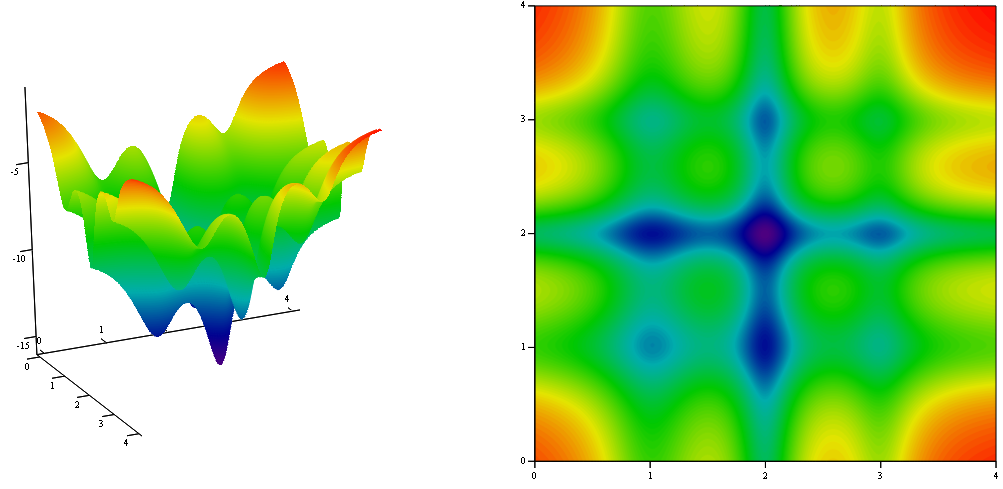
\includegraphics [scale=0.5] {MHL_TestFunction_AdditivePotential}
  \caption{Аддитивная потенциальная функция} 
  \label{TestFunctions:img:MHL_TestFunction_AdditivePotentiale}  
\end{figure}

\subsection {Параметры для алгоритмов оптимизации}

\begin{tabularwide}
\textbf{Точность вычислений:} & $\varepsilon=0.01$. \\
\textbf{Число интервалов, на которые предполагается разбивать каждую компоненту вектора $\bar{x}$ в пределах своего изменения} (для алгоритмов дискретной оптимизации) : & $NumberOfParts_j=4095$ ($j=\overline{1,n}$). \\
\textbf{Для этого длина бинарной строки для $x_j$ координаты равна} (для алгоритмов бинарной оптимизации) : & $\left( k_2\right)_j=12$ ($j=\overline{1,n}$). \\
\end{tabularwide}

\textbf{Замечание:}  $NumberOfParts_j$ выбирается как минимальное число, удовлетворяющее соотношению:
\begin{equation*}
NumberOfParts_j=2^{\left( k_2\right)_j }-1\geq\dfrac{10\left( Right_j-Left_j\right) }{\varepsilon},\text{где } \left( k_2\right)_j \in \mathbb{N}, \left( j=\overline{1,n}\right).
\end{equation*}

\subsection {Основная задача и подзадачи}

\begin{tabularwide}
\textbf{Изменяемый параметр: } & $n$ --- размерность вещественного вектора. \\
\textbf{Значение в основной задаче:} & $n=2$.\\
\end{tabularwide}

\subsection {Нахождение ошибки оптимизации}

Пусть в результате работы алгоритма оптимизации за $N$ запусков мы нашли решения $\bar{x}_{submin}^k$ со значениями целевой функции $f\left( \bar{x}_{submin}^k\right) $ соответственно ($k=\overline{1,N}$). Используем три вида ошибок:

\textbf{Надёжность: }
\begin{equation*}
R = \dfrac{\sum_{k=1}^{N}S\left( \bar{x}_{submin}^k \right) }{N}, \text{ где}
\end{equation*}
\begin{equation*}
S\left( \bar{x}_{submin}^k \right)=\left\lbrace \begin{aligned} 1,& \text{ если } \left| \left( \bar{x}_{submin}^k \right)_j-\left( \bar{x}_{min} \right)_j\right|<\varepsilon, j=\overline{1,n};   \\ 0,& \text{ иначе}. \end{aligned}\right.
\end{equation*}

\textbf{Ошибка по входным параметрам:}
\begin{equation*}
E_x = \dfrac{\sum_{k=1}^{N} \left( \frac{\sqrt{\sum_{j=1}^{n}{\left( \left( \bar{x}_{submin}^k \right)_j-\left( \bar{x}_{min} \right)_j \right)}^2 }}{n} \right)  }{N}.
\end{equation*}

\textbf{Ошибка по значениям целевой функции: }
\begin{equation*}
E_f = \dfrac{\sum_{k=1}^{N} \left| f\left( \bar{x}_{submin}^k \right)-f\left( \bar{x}_{min} \right) \right|  }{N}.
\end{equation*}

\subsection {Свойства задачи}
\begin{tabularwide}
\textbf{Условной или безусловной оптимизации: } & Задача безусловной оптимизации. \\
\textbf{Одномерной или многомерной оптимизации: } & Многомерной (двумерной). \\
\textbf{Функция унимодальная или многоэкстремальная: } & Функция многоэкстремальная. \\
\textbf{Функция стохастическая или нет: } & Функция не стохастическая. \\
\textbf{Особенности: } & Нет. \\
\end{tabularwide}

\subsection {Реализация}

Реализация функции взята из библиотеки HarrixMathLibrary в разделе <<Тестовые функции для оптимизации>>, которую можно найти по адресу \href{https://github.com/Harrix/HarrixMathLibrary} {https://github.com/Harrix/HarrixMathLibrary}.

\begin{lstlisting}[caption=Код функции MHL\_TestFunction\_AdditivePotential]
double MHL_TestFunction_AdditivePotential(double x, double y)
{
/*
Функция двух переменных: аддитивная потенциальная функция.
Тестовая функция вещественной оптимизации.
Входные параметры:
 x - первая вещественная переменная;
 y - вторая вещественная переменная.
Возвращаемое значение:
 Значение тестовой функции в точке (x,y).
*/
double VMHL_Result;
double z1=-(1./((x-1.)*(x-1.)+0.2))-(1./(2.*(x-2.)*(x-2.)+0.15))-(1./(3.*(x-3.)*(x-3.)+0.3));
double z2=-(1./((y-1.)*(y-1.)+0.2))-(1./(2.*(y-2.)*(y-2.)+0.15))-(1./(3.*(y-3.)*(y-3.)+0.3));
VMHL_Result=z1+z2;
return VMHL_Result;
}
\end{lstlisting}

\subsection {Ссылки}

Данная функция приводится в следующих источниках:

\begin{enumerate}
\item \cite[стр. 33]{book:Semenkin2007} ---  \href{http://files.lib.sfu-kras.ru/ebibl/umkd/22/u_lectures.pdf}{Эволюционные методы моделирования и оптимизации сложных систем}.
\end{enumerate}
\section {Функция Egg Holder}

\subsection {Описание функции}

\begin{tabularwide}
\textbf{Идентификатор:} & MHL\_TestFunction\_EggHolder. \\
\textbf{Наименование:} & Функция Egg Holder. \\
\textbf{Тип:} & Задача вещественной оптимизации. \\
\end{tabularwide}

\textbf{Формула} (целевая функция):
\begin{equation}
\label{TestFunctions:eq:MHL_TestFunction_EggHolder}
f\left( \bar{x}\right) = -\bar{x}_1\sin\left( \sqrt{\left| \bar{x}_1-47-\bar{x}_2\right| }\right)- (\bar{x}_2+47)\sin\left( \sqrt{\left| \dfrac{\bar{x}_1}{2}+47+\bar{x}_2\right| }\right), \text{ где}
\end{equation}
\indent $\bar{x}\in X$, $\bar{x}_j\in \left[ Left_j; Right_j\right] $, $Left_j=-512$, $Right_j=512$, $j=\overline{1,n}$, $n=2$.

\begin{tabularwide}
\textbf{Обозначение:} &\specialcell{$\bar{x}$ --- вещественный вектор;\\$n = 2$ --- размерность вещественного вектора.}  \\
\textbf{Решаемая задача оптимизации:} & $\bar{x}_{min}= \arg \min_{\bar{x}\in X} f\left( \bar{x}\right)$.   \\
\textbf{Точка минимума:} & $\bar{x}_{min}={\left( 512, 404.2319\right)}^\mathrm{T} $.    \\
\textbf{Минимум функции:} & $f\left(\bar{x}_{min} \right) =-959.64067$.   \\
\textbf{График:} & Рисунок \ref{TestFunctions:img:MHL_TestFunction_EggHoldere} нас \pageref{TestFunctions:img:MHL_TestFunction_EggHoldere} стр.   \\
\end{tabularwide}

\begin{figure} [h] 
  \center
  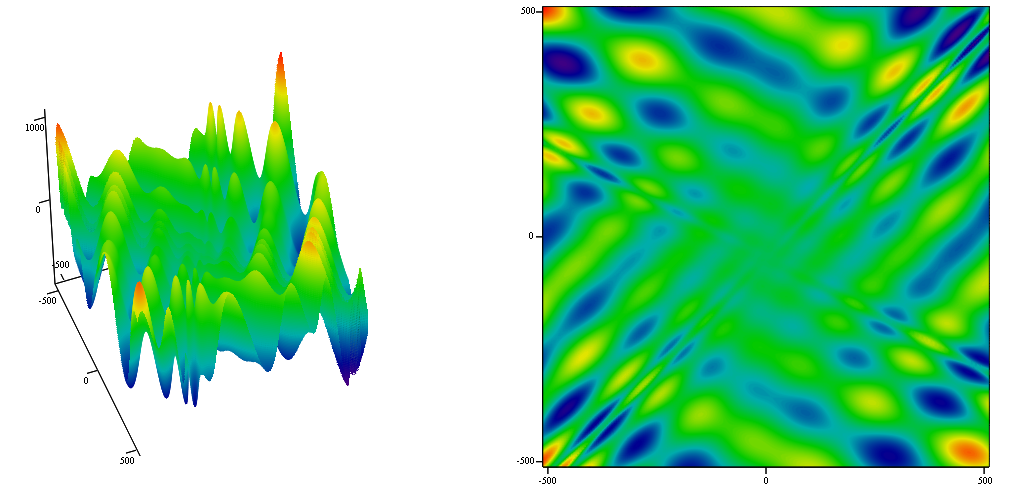
\includegraphics [scale=0.5] {MHL_TestFunction_EggHolder}
  \caption{Функция Egg Holder} 
  \label{TestFunctions:img:MHL_TestFunction_EggHoldere}  
\end{figure}

\subsection {Параметры для алгоритмов оптимизации}

\begin{tabularwide}
\textbf{Точность вычислений:} & $\varepsilon=2.5$. \\
\textbf{Число интервалов, на которые предполагается разбивать каждую компоненту вектора $\bar{x}$ в пределах своего изменения} (для алгоритмов дискретной оптимизации) : & $NumberOfParts_j=4095$ ($j=\overline{1,n}$). \\
\textbf{Для этого длина бинарной строки для $x_j$ координаты равна} (для алгоритмов бинарной оптимизации) : & $\left( k_2\right)_j=12$ ($j=\overline{1,n}$). \\
\end{tabularwide}

\textbf{Замечание:}  $NumberOfParts_j$ выбирается как минимальное число, удовлетворяющее соотношению:
\begin{equation*}
NumberOfParts_j=2^{\left( k_2\right)_j }-1\geq\dfrac{10\left( Right_j-Left_j\right) }{\varepsilon},\text{где } \left( k_2\right)_j \in \mathbb{N}, \left( j=\overline{1,n}\right).
\end{equation*}

\subsection {Основная задача и подзадачи}

\begin{tabularwide}
\textbf{Изменяемый параметр: } & $n$ --- размерность вещественного вектора. \\
\textbf{Значение в основной задаче:} & $n=2$.\\
\end{tabularwide}

\subsection {Нахождение ошибки оптимизации}

Пусть в результате работы алгоритма оптимизации за $N$ запусков мы нашли решения $\bar{x}_{submin}^k$ со значениями целевой функции $f\left( \bar{x}_{submin}^k\right) $ соответственно ($k=\overline{1,N}$). Используем три вида ошибок:

\textbf{Надёжность: }
\begin{equation*}
R = \dfrac{\sum_{k=1}^{N}S\left( \bar{x}_{submin}^k \right) }{N}, \text{ где}
\end{equation*}
\begin{equation*}
S\left( \bar{x}_{submin}^k \right)=\left\lbrace \begin{aligned} 1,& \text{ если } \left| \left( \bar{x}_{submin}^k \right)_j-\left( \bar{x}_{min} \right)_j\right|<\varepsilon, j=\overline{1,n};   \\ 0,& \text{ иначе}. \end{aligned}\right.
\end{equation*}

\textbf{Ошибка по входным параметрам:}
\begin{equation*}
E_x = \dfrac{\sum_{k=1}^{N} \left( \frac{\sqrt{\sum_{j=1}^{n}{\left( \left( \bar{x}_{submin}^k \right)_j-\left( \bar{x}_{min} \right)_j \right)}^2 }}{n} \right)  }{N}.
\end{equation*}

\textbf{Ошибка по значениям целевой функции: }
\begin{equation*}
E_f = \dfrac{\sum_{k=1}^{N} \left| f\left( \bar{x}_{submin}^k \right)-f\left( \bar{x}_{min} \right) \right|  }{N}.
\end{equation*}

\subsection {Свойства задачи}
\begin{tabularwide}
\textbf{Условной или безусловной оптимизации: } & Задача безусловной оптимизации. \\
\textbf{Одномерной или многомерной оптимизации: } & Многомерной (двумерной). \\
\textbf{Функция унимодальная или многоэкстремальная: } & Функция многоэкстремальная. \\
\textbf{Функция стохастическая или нет: } & Функция не стохастическая. \\
\textbf{Особенности: } & Нет. \\
\end{tabularwide}

\subsection {Реализация}

Реализация функции взята из библиотеки HarrixMathLibrary в разделе <<Тестовые функции для оптимизации>>, которую можно найти по адресу \href{https://github.com/Harrix/HarrixMathLibrary} {https://github.com/Harrix/HarrixMathLibrary}.

\begin{lstlisting}[caption=Код функции MHL\_TestFunction\_EggHolder]
double MHL_TestFunction_EggHolder(double x, double y)
{
/*
Функция двух переменных: функция Egg Holder.
Тестовая функция вещественной оптимизации.
Входные параметры:
 x - первая вещественная переменная;
 y - вторая вещественная переменная.
Возвращаемое значение:
 Значение тестовой функции в точке (x,y).
*/
double VMHL_Result;

VMHL_Result=-x*sin(sqrt(fabs(x-(y+47.))))-(y+47)*sin(sqrt(fabs(x/2.+47+y)));

return VMHL_Result;
}
\end{lstlisting}

\subsection {Ссылки}

Данная функция приводится в следующих источниках:

\begin{enumerate}
\item \cite[стр. 15]{article:2013arXiv1308.4008J} ---  \href{http://arxiv.org/pdf/1308.4008.pdf}{A Literature Survey of Benchmark Functions For Global Optimization Problems}.
\end{enumerate}
\section {Функция Химмельблау}
\label{TestFunctions:section:MHL_TestFunction_Himmelblau}
\subsection {Описание функции}

\begin{tabularwide}
\textbf{Идентификатор:} & MHL\_TestFunction\_Himmelblau. \\
\textbf{Наименование:} & Функция Химмельблау. \\
\textbf{Тип:} & Задача вещественной оптимизации. \\
\end{tabularwide}

\textbf{Формула} (целевая функция):
\begin{equation}
\label{TestFunctions:eq:MHL_TestFunction_Himmelblau}
f\left( \bar{x}\right) = \left( \bar{x}_1^2+\bar{x}_2-11\right)^2+\left( \bar{x}_1+\bar{x}^2-7\right)^2 , \text{ где}
\end{equation}
\indent $\bar{x}\in X$, $\bar{x}_j\in \left[ Left_j; Right_j\right] $, $Left_j=-5$, $Right_j=5$, $j=\overline{1,n}$, $n=2$.

\begin{tabularwide}
\textbf{Обозначение:} &\specialcell{$\bar{x}$ --- вещественный вектор;\\$n = 2$ --- размерность вещественного вектора.}  \\
\textbf{Решаемая задача оптимизации:} & $\bar{x}_{min}= \arg \min_{\bar{x}\in X} f\left( \bar{x}\right)$.   \\
\textbf{Точки минимума:} & \specialcell{$\bar{x}_{min}^1={\left( 3, 2\right)}^\mathrm{T} $, \\$\bar{x}_{min}^2\approx{\left( -2.8051183, 3.131312\right)}^\mathrm{T} $\\$\bar{x}_{min}^3\approx{\left( -3.779310, -3.283186\right)}^\mathrm{T} $\\$\bar{x}_{min}^4\approx{\left( 3.584428, -1.848126\right)}^\mathrm{T} $.}    \\
\textbf{Минимум функции:} & $f\left(\bar{x}_{min}^i \right) =0$, $i=\overline{1,4}$.   \\
\textbf{График:} & Рисунок \ref{TestFunctions:img:MHL_TestFunction_Himmelblaue} нас \pageref{TestFunctions:img:MHL_TestFunction_Himmelblaue} стр.   \\
\end{tabularwide}

\begin{figure} [h] 
  \center
  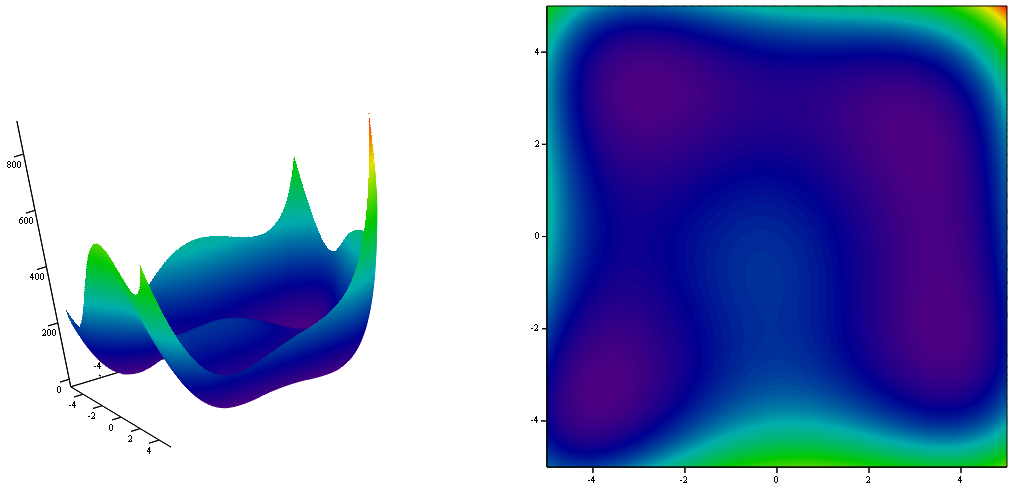
\includegraphics [scale=0.5] {MHL_TestFunction_Himmelblau}
  \caption{Функция Химмельблау} 
  \label{TestFunctions:img:MHL_TestFunction_Himmelblaue}  
\end{figure}

\subsection {Параметры для алгоритмов оптимизации}

\begin{tabularwide}
\textbf{Точность вычислений:} & $\varepsilon=0.025$. \\
\textbf{Число интервалов, на которые предполагается разбивать каждую компоненту вектора $\bar{x}$ в пределах своего изменения} (для алгоритмов дискретной оптимизации) : & $NumberOfParts_j=4095$ ($j=\overline{1,n}$). \\
\textbf{Для этого длина бинарной строки для $x_j$ координаты равна} (для алгоритмов бинарной оптимизации) : & $\left( k_2\right)_j=12$ ($j=\overline{1,n}$). \\
\end{tabularwide}

\textbf{Замечание:}  $NumberOfParts_j$ выбирается как минимальное число, удовлетворяющее соотношению:
\begin{equation*}
NumberOfParts_j=2^{\left( k_2\right)_j }-1\geq\dfrac{10\left( Right_j-Left_j\right) }{\varepsilon},\text{где } \left( k_2\right)_j \in \mathbb{N}, \left( j=\overline{1,n}\right).
\end{equation*}

\subsection {Основная задача и подзадачи}

\begin{tabularwide}
\textbf{Изменяемый параметр: } & $n$ --- размерность вещественного вектора. \\
\textbf{Значение в основной задаче:} & $n=2$.\\
\end{tabularwide}

\subsection {Нахождение ошибки оптимизации}

{\color{red} \textbf{Внимание!} В отличии от других функций формулы нахождения ошибок другие, так как есть несколько идентичных по значению целевой функции глобальных минимумов.}

Пусть в результате работы алгоритма оптимизации за $N$ запусков мы нашли решения $\bar{x}_{submin}^k$ со значениями целевой функции $f\left( \bar{x}_{submin}^k\right) $ соответственно ($k=\overline{1,N}$). Используем три вида ошибок:

\textbf{Надёжность: }
\begin{equation*}
R = \dfrac{\sum_{k=1}^{N}S\left( \bar{x}_{submin}^k \right) }{N}, \text{ где}
\end{equation*}
\begin{equation*}
S\left( \bar{x}_{submin}^k \right)=\left\lbrace \begin{aligned} 1,& \text{ если } \left| \left( \bar{x}_{submin}^k \right)_j-\left( \bar{x}_{min}^1 \right)_j\right|<\varepsilon, j=\overline{1,n};   \\ 1,& \text{ если } \left| \left( \bar{x}_{submin}^k \right)_j-\left( \bar{x}_{min}^2 \right)_j\right|<\varepsilon, j=\overline{1,n};   \\ 1,& \text{ если } \left| \left( \bar{x}_{submin}^k \right)_j-\left( \bar{x}_{min}^3 \right)_j\right|<\varepsilon, j=\overline{1,n};   \\ 1,& \text{ если } \left| \left( \bar{x}_{submin}^k \right)_j-\left( \bar{x}_{min}^4 \right)_j\right|<\varepsilon, j=\overline{1,n};   \\ 0,& \text{ иначе}. \end{aligned}\right.
\end{equation*}

\textbf{Ошибка по входным параметрам:}
\begin{equation*}
E_x = \min_{i=\overline{1,4}} \left\lbrace  \frac{\sum_{k=1}^{N} \left( \frac{\sqrt{\sum_{j=1}^{n}{\left( \left( \bar{x}_{submin}^k \right)_j-\left( \bar{x}_{min}^i \right)_j \right)}^2 }}{n} \right)  }{N}\right\rbrace  .
\end{equation*}

\textbf{Ошибка по значениям целевой функции: } (без изменений)
\begin{equation*}
E_f = \dfrac{\sum_{k=1}^{N} \left| f\left( \bar{x}_{submin}^k \right)-f\left( \bar{x}_{min} \right) \right|  }{N}.
\end{equation*}

\subsection {Свойства задачи}
\begin{tabularwide}
\textbf{Условной или безусловной оптимизации: } & Задача безусловной оптимизации. \\
\textbf{Одномерной или многомерной оптимизации: } & Многомерной: (двумерной). \\
\textbf{Функция унимодальная или многоэкстремальная: } & Функция многоэкстремальная. \\
\textbf{Функция стохастическая или нет: } & Функция не стохастическая. \\
\textbf{Особенности: } & Есть 4 глобальных минимума. \\
\end{tabularwide}

\subsection {Реализация}

Реализация функции взята из библиотеки HarrixMathLibrary в разделе <<Тестовые функции для оптимизации>>, которую можно найти по адресу \href{https://github.com/Harrix/HarrixMathLibrary} {https://github.com/Harrix/HarrixMathLibrary}.

\begin{lstlisting}[caption=Код функции MHL\_TestFunction\_Himmelblau]
double MHL_TestFunction_Himmelblau(double x, double y)
{
/*
Функция двух переменных: функция Химмельблау.
Тестовая функция вещественной оптимизации.
Входные параметры:
 x - первая вещественная переменная;
 y - вторая вещественная переменная.
Возвращаемое значение:
 Значение тестовой функции в точке (x,y).
*/
double VMHL_Result;
VMHL_Result=(x*x+y-11)*(x*x+y-11)+(x+y*y-7)*(x+y*y-7);
return VMHL_Result;
}
\end{lstlisting}

\subsection {Ссылки}

Данная функция приводится в следующих источниках:

\begin{enumerate}
\item \cite{web:Himmelblausfunction} ---  \href{http://en.wikipedia.org/wiki/Himmelblau's_function}{Himmelblau's function}.
\item \cite{web:MinimizationOfTheHimmelblauFunction} ---  \href{http://pythonhosted.org/algopy/examples/minimization/himmelblau_minimization.html}{Minimization of the Himmelblau Function}.
\end{enumerate}
\section {Перевернутая функция Розенброка}
\label{TestFunctions:section:MHL_TestFunction_InvertedRosenbrock}
\subsection {Описание функции}

\begin{tabularwide}
\textbf{Идентификатор:} & MHL\_TestFunction\_InvertedRosenbrock. \\
\textbf{Наименование:} & Перевернутая функция Розенброка. \\
\textbf{Тип:} & Задача вещественной оптимизации. \\
\end{tabularwide}

\textbf{Формула} (целевая функция):
\begin{equation}
\label{TestFunctions:eq:MHL_TestFunction_InvertedRosenbrock}
f\left( \bar{x}\right) =\dfrac{-100}{100\left( \bar{x}_1^2-\bar{x}_2\right) +\left( 1.-\bar{x}_1\right)^2+600}, \text{ где}
\end{equation}
\indent $\bar{x}\in X$, $\bar{x}_j\in \left[ Left_j; Right_j\right] $, $Left_j=-5$, $Right_j=5$, $j=\overline{1,n}$, $n=2$.

\begin{tabularwide}
\textbf{Обозначение:} &\specialcell{$\bar{x}$ --- вещественный вектор;\\$n = 2$ --- размерность вещественного вектора.}  \\
\textbf{Решаемая задача оптимизации:} & $\bar{x}_{min}= \arg \min_{\bar{x}\in X} f\left( \bar{x}\right)$.   \\
\textbf{Точка минимума:} & $\bar{x}_{min}={\left( 0.00990099, 5\right)}^\mathrm{T} $.    \\
\textbf{Минимум функции:} & $f\left(\bar{x}_{min} \right) =-0.99019608$.   \\
\textbf{График:} & Рисунок \ref{TestFunctions:img:MHL_TestFunction_InvertedRosenbrocke} нас \pageref{TestFunctions:img:MHL_TestFunction_InvertedRosenbrocke} стр.   \\
\end{tabularwide}

\begin{figure} [h] 
  \center
  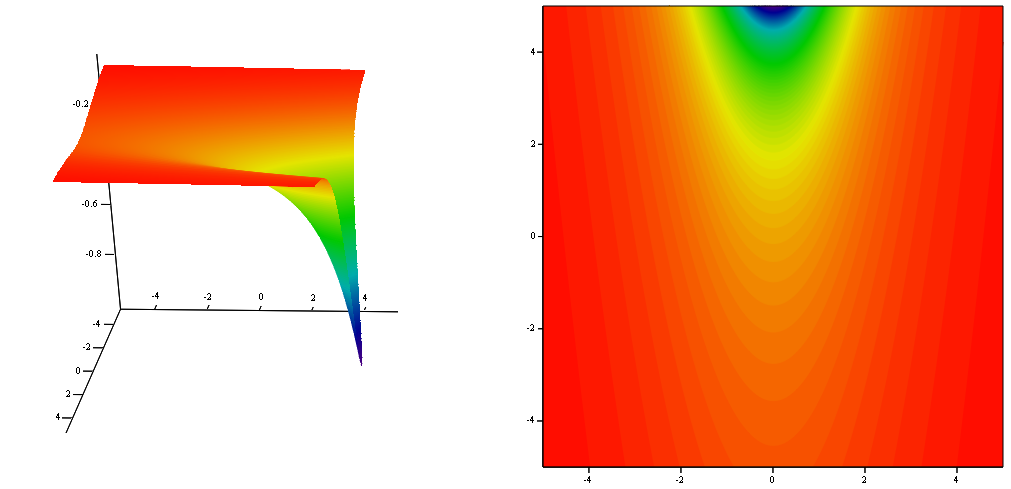
\includegraphics [scale=0.5] {MHL_TestFunction_InvertedRosenbrock}
  \caption{Перевернутая функция Розенброка} 
  \label{TestFunctions:img:MHL_TestFunction_InvertedRosenbrocke}  
\end{figure}

\subsection {Параметры для алгоритмов оптимизации}

\begin{tabularwide}
\textbf{Точность вычислений:} & $\varepsilon=0.025$. \\
\textbf{Число интервалов, на которые предполагается разбивать каждую компоненту вектора $\bar{x}$ в пределах своего изменения} (для алгоритмов дискретной оптимизации) : & $NumberOfParts_j=4095$ ($j=\overline{1,n}$). \\
\textbf{Для этого длина бинарной строки для $x_j$ координаты равна} (для алгоритмов бинарной оптимизации) : & $\left( k_2\right)_j=12$ ($j=\overline{1,n}$). \\
\end{tabularwide}

\textbf{Замечание:}  $NumberOfParts_j$ выбирается как минимальное число, удовлетворяющее соотношению:
\begin{equation*}
NumberOfParts_j=2^{\left( k_2\right)_j }-1\geq\dfrac{10\left( Right_j-Left_j\right) }{\varepsilon},\text{где } \left( k_2\right)_j \in \mathbb{N}, \left( j=\overline{1,n}\right).
\end{equation*}

\subsection {Основная задача и подзадачи}

\begin{tabularwide}
\textbf{Изменяемый параметр: } & $n$ --- размерность вещественного вектора. \\
\textbf{Значение в основной задаче:} & $n=2$.\\
\end{tabularwide}

\subsection {Нахождение ошибки оптимизации}

Пусть в результате работы алгоритма оптимизации за $N$ запусков мы нашли решения $\bar{x}_{submin}^k$ со значениями целевой функции $f\left( \bar{x}_{submin}^k\right) $ соответственно ($k=\overline{1,N}$). Используем три вида ошибок:

\textbf{Надёжность: }
\begin{equation*}
R = \dfrac{\sum_{k=1}^{N}S\left( \bar{x}_{submin}^k \right) }{N}, \text{ где}
\end{equation*}
\begin{equation*}
S\left( \bar{x}_{submin}^k \right)=\left\lbrace \begin{aligned} 1,& \text{ если } \left| \left( \bar{x}_{submin}^k \right)_j-\left( \bar{x}_{min} \right)_j\right|<\varepsilon, j=\overline{1,n};   \\ 0,& \text{ иначе}. \end{aligned}\right.
\end{equation*}

\textbf{Ошибка по входным параметрам:}
\begin{equation*}
E_x = \dfrac{\sum_{k=1}^{N} \left( \frac{\sqrt{\sum_{j=1}^{n}{\left( \left( \bar{x}_{submin}^k \right)_j-\left( \bar{x}_{min} \right)_j \right)}^2 }}{n} \right)  }{N}.
\end{equation*}

\textbf{Ошибка по значениям целевой функции: }
\begin{equation*}
E_f = \dfrac{\sum_{k=1}^{N} \left| f\left( \bar{x}_{submin}^k \right)-f\left( \bar{x}_{min} \right) \right|  }{N}.
\end{equation*}

\subsection {Свойства задачи}
\begin{tabularwide}
\textbf{Условной или безусловной оптимизации: } & Задача безусловной оптимизации. \\
\textbf{Одномерной или многомерной оптимизации: } & Многомерной (двумерной). \\
\textbf{Функция унимодальная или многоэкстремальная: } & Функция унимодальная на рассматриваемой области. \\
\textbf{Функция стохастическая или нет: } & Функция не стохастическая. \\
\textbf{Особенности: } & Авторская модификация функции. \\
\end{tabularwide}

\subsection {Реализация}

Реализация функции взята из библиотеки HarrixMathLibrary в разделе <<Тестовые функции для оптимизации>>, которую можно найти по адресу \href{https://github.com/Harrix/HarrixMathLibrary} {https://github.com/Harrix/HarrixMathLibrary}.

\begin{lstlisting}[caption=Код функции MHL\_TestFunction\_InvertedRosenbrock]
double MHL_TestFunction_InvertedRosenbrock(double x, double y)
{
/*
Функция двух переменных: перевернутая функция Розенброка.
Тестовая функция вещественной оптимизации.
Входные параметры:
 x - первая вещественная переменная;
 y - вторая вещественная переменная.
Возвращаемое значение:
 Значение тестовой функции в точке (x,y).
*/
double VMHL_Result;

VMHL_Result=-100./(100.*(x*x-y)+(1.-x)*(1.-x)+600.);

return VMHL_Result;
}
\end{lstlisting}

\subsection {Ссылки}

Представленная здесь функция является модификацией неправильной записи функции из данного источника:

\begin{enumerate}
\item \cite[стр. 29]{book:Semenkin2007} ---  \href{http://files.lib.sfu-kras.ru/ebibl/umkd/22/u_lectures.pdf}{Эволюционные методы моделирования и оптимизации сложных систем}.
\end{enumerate}
\section {Функция Катникова}
\label{TestFunctions:section:MHL_TestFunction_Katnikov}
\subsection {Описание функции}

\begin{tabularwide}
\textbf{Идентификатор:} & MHL\_TestFunction\_Katnikov. \\
\textbf{Наименование:} & Функция Катникова. \\
\textbf{Тип:} & Задача вещественной оптимизации. \\
\end{tabularwide}

\textbf{Формула} (целевая функция):
\begin{equation}
\label{TestFunctions:eq:MHL_TestFunction_Katnikov}
f\left( \bar{x}\right) = 0.5\left( \bar{x}_1^2+\bar{x}_2^2\right) \left( 2A+A\cos\left( 1.5\bar{x}_1\right)\cos\left( 3.14\bar{x}_2\right)+A\cos\left( \sqrt{5}\bar{x}_1\right)\cos\left( 3.5\bar{x}_2\right)    \right) , \text{ где}
\end{equation}
\indent $\bar{x}\in X$, $\bar{x}_j\in \left[ Left_j; Right_j\right] $, $Left_j=-5$, $Right_j=5$, $j=\overline{1,n}$, $n=2$, $A=0.8$.

\begin{tabularwide}
\textbf{Обозначение:} &\specialcell{$\bar{x}$ --- вещественный вектор;\\$n = 2$ --- размерность вещественного вектора.}  \\
\textbf{Решаемая задача оптимизации:} & $\bar{x}_{min}= \arg \min_{\bar{x}\in X} f\left( \bar{x}\right)$.   \\
\textbf{Точка минимума:} & $\bar{x}_{min}={\left( 0, 0\right)}^\mathrm{T} $, то есть $\left(\bar{x}_{min} \right)_j=0$ ($j=\overline{1,n}$).    \\
\textbf{Минимум функции:} & $f\left(\bar{x}_{min} \right) =0$.   \\
\textbf{График:} & Рисунок \ref{TestFunctions:img:MHL_TestFunction_Katnikove} нас \pageref{TestFunctions:img:MHL_TestFunction_Katnikove} стр.   \\
\end{tabularwide}

\begin{figure} [h] 
  \center
  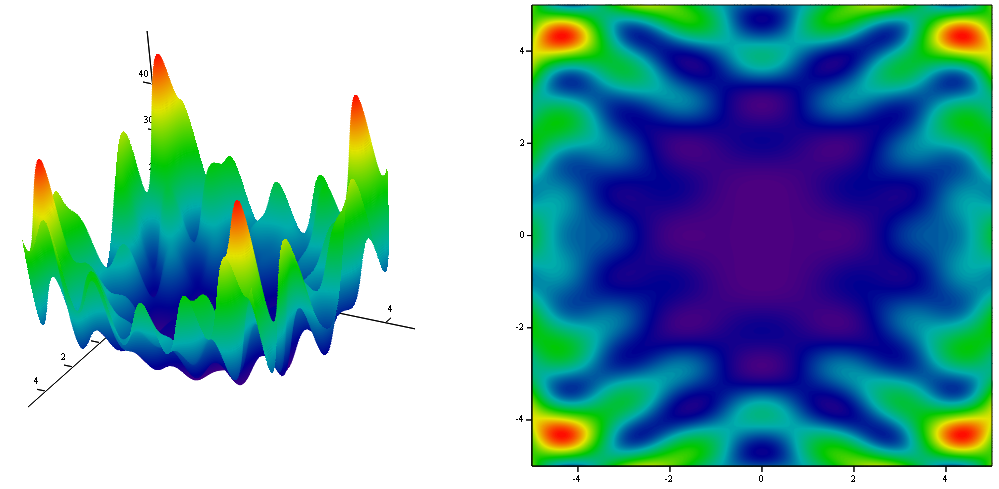
\includegraphics [scale=0.5] {MHL_TestFunction_Katnikov}
  \caption{Функция Катникова} 
  \label{TestFunctions:img:MHL_TestFunction_Katnikove}  
\end{figure}

\subsection {Параметры для алгоритмов оптимизации}

\begin{tabularwide}
\textbf{Точность вычислений:} & $\varepsilon=0.025$. \\
\textbf{Число интервалов, на которые предполагается разбивать каждую компоненту вектора $\bar{x}$ в пределах своего изменения} (для алгоритмов дискретной оптимизации) : & $NumberOfParts_j=4095$ ($j=\overline{1,n}$). \\
\textbf{Для этого длина бинарной строки для $x_j$ координаты равна} (для алгоритмов бинарной оптимизации) : & $\left( k_2\right)_j=12$ ($j=\overline{1,n}$). \\
\end{tabularwide}

\textbf{Замечание:}  $NumberOfParts_j$ выбирается как минимальное число, удовлетворяющее соотношению:
\begin{equation*}
NumberOfParts_j=2^{\left( k_2\right)_j }-1\geq\dfrac{10\left( Right_j-Left_j\right) }{\varepsilon},\text{где } \left( k_2\right)_j \in \mathbb{N}, \left( j=\overline{1,n}\right).
\end{equation*}

\subsection {Основная задача и подзадачи}

\begin{tabularwide}
\textbf{Изменяемый параметр: } & $n$ --- размерность вещественного вектора. \\
\textbf{Значение в основной задаче:} & $n=2$.\\
\end{tabularwide}

\subsection {Нахождение ошибки оптимизации}

Пусть в результате работы алгоритма оптимизации за $N$ запусков мы нашли решения $\bar{x}_{submin}^k$ со значениями целевой функции $f\left( \bar{x}_{submin}^k\right) $ соответственно ($k=\overline{1,N}$). Используем три вида ошибок:

\textbf{Надёжность: }
\begin{equation*}
R = \dfrac{\sum_{k=1}^{N}S\left( \bar{x}_{submin}^k \right) }{N}, \text{ где}
\end{equation*}
\begin{equation*}
S\left( \bar{x}_{submin}^k \right)=\left\lbrace \begin{aligned} 1,& \text{ если } \left| \left( \bar{x}_{submin}^k \right)_j-\left( \bar{x}_{min} \right)_j\right|<\varepsilon, j=\overline{1,n};   \\ 0,& \text{ иначе}. \end{aligned}\right.
\end{equation*}

\textbf{Ошибка по входным параметрам:}
\begin{equation*}
E_x = \dfrac{\sum_{k=1}^{N} \left( \frac{\sqrt{\sum_{j=1}^{n}{\left( \left( \bar{x}_{submin}^k \right)_j-\left( \bar{x}_{min} \right)_j \right)}^2 }}{n} \right)  }{N}.
\end{equation*}

\textbf{Ошибка по значениям целевой функции: }
\begin{equation*}
E_f = \dfrac{\sum_{k=1}^{N} \left| f\left( \bar{x}_{submin}^k \right)-f\left( \bar{x}_{min} \right) \right|  }{N}.
\end{equation*}

\subsection {Свойства задачи}
\begin{tabularwide}
\textbf{Условной или безусловной оптимизации: } & Задача безусловной оптимизации. \\
\textbf{Одномерной или многомерной оптимизации: } & Многомерной: (двумерной). \\
\textbf{Функция унимодальная или многоэкстремальная: } & Функция многоэкстремальная. \\
\textbf{Функция стохастическая или нет: } & Функция не стохастическая. \\
\textbf{Особенности: } & Нет. \\
\end{tabularwide}

\subsection {Реализация}

Реализация функции взята из библиотеки HarrixMathLibrary в разделе <<Тестовые функции для оптимизации>>, которую можно найти по адресу \href{https://github.com/Harrix/HarrixMathLibrary} {https://github.com/Harrix/HarrixMathLibrary}.

\begin{lstlisting}[caption=Код функции MHL\_TestFunction\_Katnikov]
double MHL_TestFunction_Katnikov(double x, double y)
{
/*
Функция двух переменных: функция Катникова.
Тестовая функция вещественной оптимизации.
Входные параметры:
 x - первая вещественная переменная;
 y - вторая вещественная переменная.
Возвращаемое значение:
 Значение тестовой функции в точке (x,y).
*/
double VMHL_Result;
double A=0.8;
VMHL_Result=0.5*(x*x+y*y)*(2*A+A*cos(1.5*x)*cos(3.14*y)+A*cos(sqrt(5)*x)*cos(3.5*y));
return VMHL_Result;
}
\end{lstlisting}

\subsection {Ссылки}

Данная функция приводится в следующих источниках:

\begin{enumerate}
\item \cite[стр. 31]{book:Semenkin2007} ---  \href{http://files.lib.sfu-kras.ru/ebibl/umkd/22/u_lectures.pdf}{Эволюционные методы моделирования и оптимизации сложных систем}.
\end{enumerate}
\section {Функция Multiextremal3}
\label{TestFunctions:section:MHL_TestFunction_Multiextremal3}
\subsection {Описание функции}

\begin{tabularwide}
\textbf{Идентификатор:} & MHL\_TestFunction\_Multiextremal3. \\
\textbf{Наименование:} & Функция Multiextremal3. \\
\textbf{Тип:} & Задача вещественной оптимизации. \\
\end{tabularwide}

\textbf{Формула} (целевая функция):
\begin{equation}
\label{TestFunctions:eq:MHL_TestFunction_Multiextremal3}
f\left( \bar{x}\right) = \bar{x}_1^2\left| \sin\left( 2\bar{x}_1\right) \right| +\bar{x}_2^2\left| \sin\left( 2\bar{x}_2\right) \right| -\dfrac{1}{5\bar{x}_1^2+5\bar{x}_2^2+0.2} + 5, \text{ где}
\end{equation}
\indent $\bar{x}\in X$, $\bar{x}_j\in \left[ Left_j; Right_j\right] $, $Left_j=-5$, $Right_j=5$, $j=\overline{1,n}$, $n=2$.

\begin{tabularwide}
\textbf{Обозначение:} &\specialcell{$\bar{x}$ --- вещественный вектор;\\$n = 2$ --- размерность вещественного вектора.}  \\
\textbf{Решаемая задача оптимизации:} & $\bar{x}_{min}= \arg \min_{\bar{x}\in X} f\left( \bar{x}\right)$.   \\
\textbf{Точка минимума:} & $\bar{x}_{min}={\left( 0, 0\right)}^\mathrm{T} $, то есть $\left(\bar{x}_{min} \right)_j=0$ ($j=\overline{1,n}$).    \\
\textbf{Минимум функции:} & $f\left(\bar{x}_{min} \right) =0$.   \\
\textbf{График:} & Рисунок \ref{TestFunctions:img:MHL_TestFunction_Multiextremal3e} нас \pageref{TestFunctions:img:MHL_TestFunction_Multiextremal3e} стр.   \\
\end{tabularwide}

\begin{figure} [h] 
  \center
  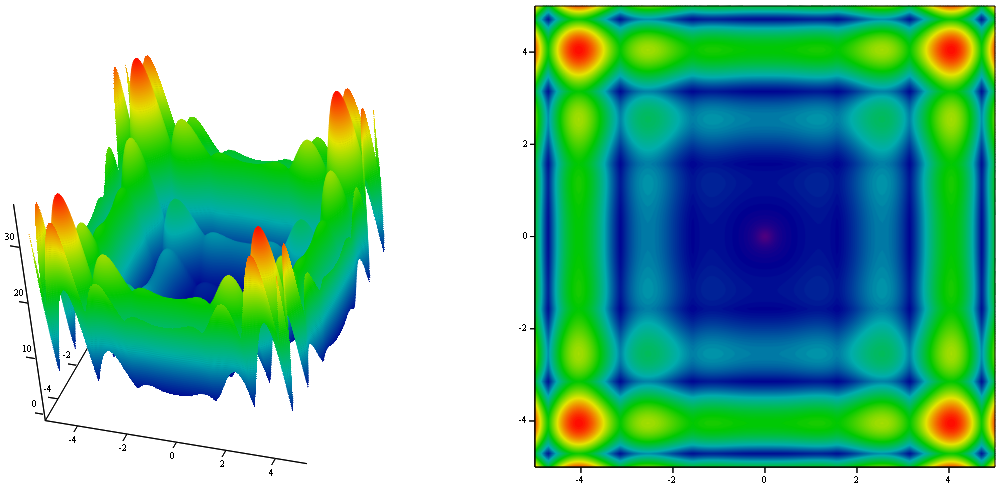
\includegraphics [scale=0.5] {MHL_TestFunction_Multiextremal3}
  \caption{Функция Multiextremal3} 
  \label{TestFunctions:img:MHL_TestFunction_Multiextremal3e}  
\end{figure}

\subsection {Параметры для алгоритмов оптимизации}

\begin{tabularwide}
\textbf{Точность вычислений:} & $\varepsilon=0.025$. \\
\textbf{Число интервалов, на которые предполагается разбивать каждую компоненту вектора $\bar{x}$ в пределах своего изменения} (для алгоритмов дискретной оптимизации) : & $NumberOfParts_j=4095$ ($j=\overline{1,n}$). \\
\textbf{Для этого длина бинарной строки для $x_j$ координаты равна} (для алгоритмов бинарной оптимизации) : & $\left( k_2\right)_j=12$ ($j=\overline{1,n}$). \\
\end{tabularwide}

\textbf{Замечание:}  $NumberOfParts_j$ выбирается как минимальное число, удовлетворяющее соотношению:
\begin{equation*}
NumberOfParts_j=2^{\left( k_2\right)_j }-1\geq\dfrac{10\left( Right_j-Left_j\right) }{\varepsilon},\text{где } \left( k_2\right)_j \in \mathbb{N}, \left( j=\overline{1,n}\right).
\end{equation*}

\subsection {Основная задача и подзадачи}

\begin{tabularwide}
\textbf{Изменяемый параметр: } & $n$ --- размерность вещественного вектора. \\
\textbf{Значение в основной задаче:} & $n=2$.\\
\end{tabularwide}

\subsection {Нахождение ошибки оптимизации}

Пусть в результате работы алгоритма оптимизации за $N$ запусков мы нашли решения $\bar{x}_{submin}^k$ со значениями целевой функции $f\left( \bar{x}_{submin}^k\right) $ соответственно ($k=\overline{1,N}$). Используем три вида ошибок:

\textbf{Надёжность: }
\begin{equation*}
R = \dfrac{\sum_{k=1}^{N}S\left( \bar{x}_{submin}^k \right) }{N}, \text{ где}
\end{equation*}
\begin{equation*}
S\left( \bar{x}_{submin}^k \right)=\left\lbrace \begin{aligned} 1,& \text{ если } \left| \left( \bar{x}_{submin}^k \right)_j-\left( \bar{x}_{min} \right)_j\right|<\varepsilon, j=\overline{1,n};   \\ 0,& \text{ иначе}. \end{aligned}\right.
\end{equation*}

\textbf{Ошибка по входным параметрам:}
\begin{equation*}
E_x = \dfrac{\sum_{k=1}^{N} \left( \frac{\sqrt{\sum_{j=1}^{n}{\left( \left( \bar{x}_{submin}^k \right)_j-\left( \bar{x}_{min} \right)_j \right)}^2 }}{n} \right)  }{N}.
\end{equation*}

\textbf{Ошибка по значениям целевой функции: }
\begin{equation*}
E_f = \dfrac{\sum_{k=1}^{N} \left| f\left( \bar{x}_{submin}^k \right)-f\left( \bar{x}_{min} \right) \right|  }{N}.
\end{equation*}

\subsection {Свойства задачи}
\begin{tabularwide}
\textbf{Условной или безусловной оптимизации: } & Задача безусловной оптимизации. \\
\textbf{Одномерной или многомерной оптимизации: } & Многомерной: (двумерной). \\
\textbf{Функция унимодальная или многоэкстремальная: } & Функция многоэкстремальная. \\
\textbf{Функция стохастическая или нет: } & Функция не стохастическая. \\
\textbf{Особенности: } & Нет. \\
\end{tabularwide}

\subsection {Реализация}

Реализация функции взята из библиотеки HarrixMathLibrary в разделе <<Тестовые функции для оптимизации>>, которую можно найти по адресу \href{https://github.com/Harrix/HarrixMathLibrary} {https://github.com/Harrix/HarrixMathLibrary}.

\begin{lstlisting}[caption=Код функции MHL\_TestFunction\_Multiextremal3]
double MHL_TestFunction_Multiextremal3(double x, double y)
{
/*
Функция двух переменных: функция Multiextremal3.
Тестовая функция вещественной оптимизации.
Входные параметры:
 x - первая вещественная переменная;
 y - вторая вещественная переменная.
Возвращаемое значение:
 Значение тестовой функции в точке (x,y).
*/
double VMHL_Result;
VMHL_Result=x*x*fabs(sin(2.*x))+y*y*fabs(sin(2.*y))-1./(5.*x*x+5.*y*y+0.2)+5.;
return VMHL_Result;
}
\end{lstlisting}

\subsection {Ссылки}

Данная функция приводится в следующих источниках:

\begin{enumerate}
\item \cite[стр. 31]{book:Semenkin2007} ---  \href{http://files.lib.sfu-kras.ru/ebibl/umkd/22/u_lectures.pdf}{Эволюционные методы моделирования и оптимизации сложных систем}.
\end{enumerate}
\section {Функция Multiextremal4}
\label{TestFunctions:section:MHL_TestFunction_Multiextremal4}
\subsection {Описание функции}

\begin{tabularwide}
\textbf{Идентификатор:} & MHL\_TestFunction\_Multiextremal4. \\
\textbf{Наименование:} & Функция Multiextremal4. \\
\textbf{Тип:} & Задача вещественной оптимизации. \\
\end{tabularwide}

\textbf{Формула} (целевая функция):
\begin{align}
\label{TestFunctions:eq:MHL_TestFunction_Multiextremal4}
f\left( \bar{x}\right) =& 0.5\left( \bar{x}_1^2+\bar{x}_1\bar{x}_2 +\bar{x}_2^2\right) \left( 1+0.5\cos\left(1.5\bar{x}_1\right)\cos\left(3.2\bar{x}_1\bar{x}_2\right)\cos\left(3.14\bar{x}_2\right)  +\right. \\
 & \left.+0.5\cos\left(2.2\bar{x}_1\right)\cos\left(4.8\bar{x}_1\bar{x}_2\right)\cos\left(3.5\bar{x}_2\right)\right), \text{ где}\nonumber
\end{align}
\indent $\bar{x}\in X$, $\bar{x}_j\in \left[ Left_j; Right_j\right] $, $Left_j=0$, $Right_j=4$, $j=\overline{1,n}$, $n=2$.

\begin{tabularwide}
\textbf{Обозначение:} &\specialcell{$\bar{x}$ --- вещественный вектор;\\$n = 2$ --- размерность вещественного вектора.}  \\
\textbf{Решаемая задача оптимизации:} & $\bar{x}_{min}= \arg \min_{\bar{x}\in X} f\left( \bar{x}\right)$.   \\
\textbf{Точка минимума:} & $\bar{x}_{min}={\left( 0, 0\right)}^\mathrm{T} $, то есть $\left(\bar{x}_{min} \right)_j=0$ ($j=\overline{1,n}$).    \\
\textbf{Минимум функции:} & $f\left(\bar{x}_{min} \right) =0$.   \\
\textbf{График:} & Рисунок \ref{TestFunctions:img:MHL_TestFunction_Multiextremal4e} нас \pageref{TestFunctions:img:MHL_TestFunction_Multiextremal4e} стр.   \\
\end{tabularwide}

\begin{figure} [h] 
  \center
  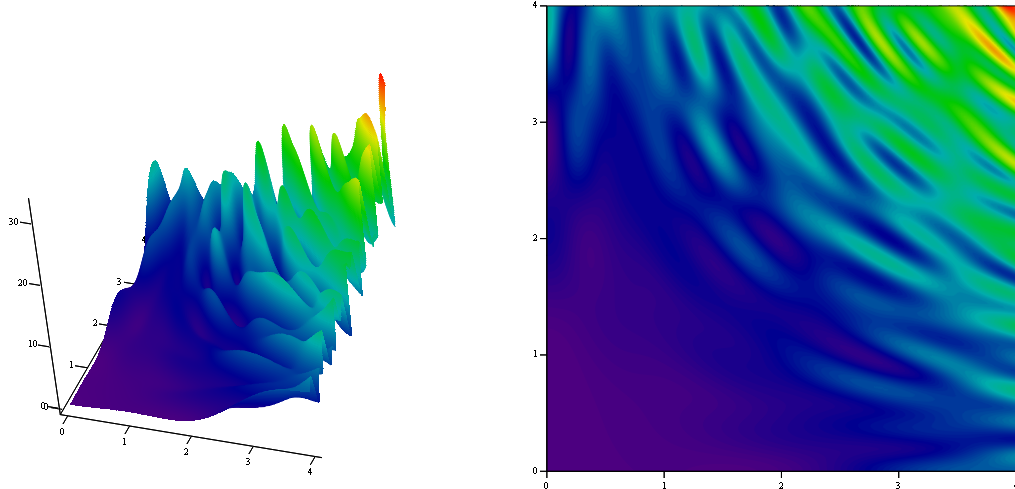
\includegraphics [scale=0.5] {MHL_TestFunction_Multiextremal4}
  \caption{Функция Multiextremal4} 
  \label{TestFunctions:img:MHL_TestFunction_Multiextremal4e}  
\end{figure}

\subsection {Параметры для алгоритмов оптимизации}

\begin{tabularwide}
\textbf{Точность вычислений:} & $\varepsilon=0.01$. \\
\textbf{Число интервалов, на которые предполагается разбивать каждую компоненту вектора $\bar{x}$ в пределах своего изменения} (для алгоритмов дискретной оптимизации) : & $NumberOfParts_j=4095$ ($j=\overline{1,n}$). \\
\textbf{Для этого длина бинарной строки для $x_j$ координаты равна} (для алгоритмов бинарной оптимизации) : & $\left( k_2\right)_j=12$ ($j=\overline{1,n}$). \\
\end{tabularwide}

\textbf{Замечание:}  $NumberOfParts_j$ выбирается как минимальное число, удовлетворяющее соотношению:
\begin{equation*}
NumberOfParts_j=2^{\left( k_2\right)_j }-1\geq\dfrac{10\left( Right_j-Left_j\right) }{\varepsilon},\text{где } \left( k_2\right)_j \in \mathbb{N}, \left( j=\overline{1,n}\right).
\end{equation*}

\subsection {Основная задача и подзадачи}

\begin{tabularwide}
\textbf{Изменяемый параметр: } & $n$ --- размерность вещественного вектора. \\
\textbf{Значение в основной задаче:} & $n=2$.\\
\end{tabularwide}

\subsection {Нахождение ошибки оптимизации}

Пусть в результате работы алгоритма оптимизации за $N$ запусков мы нашли решения $\bar{x}_{submin}^k$ со значениями целевой функции $f\left( \bar{x}_{submin}^k\right) $ соответственно ($k=\overline{1,N}$). Используем три вида ошибок:

\textbf{Надёжность: }
\begin{equation*}
R = \dfrac{\sum_{k=1}^{N}S\left( \bar{x}_{submin}^k \right) }{N}, \text{ где}
\end{equation*}
\begin{equation*}
S\left( \bar{x}_{submin}^k \right)=\left\lbrace \begin{aligned} 1,& \text{ если } \left| \left( \bar{x}_{submin}^k \right)_j-\left( \bar{x}_{min} \right)_j\right|<\varepsilon, j=\overline{1,n};   \\ 0,& \text{ иначе}. \end{aligned}\right.
\end{equation*}

\textbf{Ошибка по входным параметрам:}
\begin{equation*}
E_x = \dfrac{\sum_{k=1}^{N} \left( \frac{\sqrt{\sum_{j=1}^{n}{\left( \left( \bar{x}_{submin}^k \right)_j-\left( \bar{x}_{min} \right)_j \right)}^2 }}{n} \right)  }{N}.
\end{equation*}

\textbf{Ошибка по значениям целевой функции: }
\begin{equation*}
E_f = \dfrac{\sum_{k=1}^{N} \left| f\left( \bar{x}_{submin}^k \right)-f\left( \bar{x}_{min} \right) \right|  }{N}.
\end{equation*}

\subsection {Свойства задачи}
\begin{tabularwide}
\textbf{Условной или безусловной оптимизации: } & Задача безусловной оптимизации. \\
\textbf{Одномерной или многомерной оптимизации: } & Многомерной: (двумерной). \\
\textbf{Функция унимодальная или многоэкстремальная: } & Функция многоэкстремальная. \\
\textbf{Функция стохастическая или нет: } & Функция не стохастическая. \\
\textbf{Особенности: } & Нет. \\
\end{tabularwide}

\subsection {Реализация}

Реализация функции взята из библиотеки HarrixMathLibrary в разделе <<Тестовые функции для оптимизации>>, которую можно найти по адресу \href{https://github.com/Harrix/HarrixMathLibrary} {https://github.com/Harrix/HarrixMathLibrary}.

\begin{lstlisting}[caption=Код функции MHL\_TestFunction\_Multiextremal4]
double MHL_TestFunction_Multiextremal4(double x, double y)
{
/*
Функция двух переменных: функция Multiextremal4.
Тестовая функция вещественной оптимизации.
Входные параметры:
 x - первая вещественная переменная;
 y - вторая вещественная переменная.
Возвращаемое значение:
 Значение тестовой функции в точке (x,y).
*/
double VMHL_Result;
VMHL_Result=0.5*(x*x+x*y+y*y)*(1.+0.5*cos(1.5*x)*cos(3.2*x*y)*cos(3.14*y)+0.5*cos(2.2*x)*cos(4.8*x*y)*cos(3.5*y));
return VMHL_Result;
}
\end{lstlisting}

\subsection {Ссылки}

Данная функция приводится в следующих источниках:

\begin{enumerate}
\item \cite[стр. 31]{book:Semenkin2007} ---  \href{http://files.lib.sfu-kras.ru/ebibl/umkd/22/u_lectures.pdf}{Эволюционные методы моделирования и оптимизации сложных систем}.
\end{enumerate}
\section {Мультипликативная потенциальная функция}

\subsection {Описание функции}

\begin{tabularwide}
\textbf{Идентификатор:} & MHL\_TestFunction\_MultiplicativePotential. \\
\textbf{Наименование:} & Мультипликативная потенциальная функция. \\
\textbf{Тип:} & Задача вещественной оптимизации. \\
\end{tabularwide}

\textbf{Формула} (целевая функция):
\begin{equation}
\label{TestFunctions:eq:MHL_MultiplicativePotential}
f\left( \bar{x}\right) = -z\left( \bar{x}_1\right)\cdot z\left( \bar{x}_2\right), \text{ где}
\end{equation}
\begin{equation*}
\label{TestFunctions:eq:MHL_MultiplicativePotential2}
z\left( v\right)= -\dfrac{1}{\left( v-1\right)^2+0.2 }-\dfrac{1}{2\left( v-2\right)^2+0.15}-\dfrac{1}{3\left( v-3\right)^2+0.3},
\end{equation*}
\indent $\bar{x}\in X$, $\bar{x}_j\in \left[ Left_j; Right_j\right] $, $Left_j=0$, $Right_j=4$, $j=\overline{1,n}$, $n=2$.

\begin{tabularwide}
\textbf{Обозначение:} &\specialcell{$\bar{x}$ --- вещественный вектор;\\$n = 2$ --- размерность вещественного вектора.}  \\
\textbf{Решаемая задача оптимизации:} & $\bar{x}_{min}= \arg \min_{\bar{x}\in X} f\left( \bar{x}\right)$.   \\
\textbf{Точка минимума:} & $\bar{x}_{min}={\left( 2, 2\right)}^\mathrm{T} $, то есть $\left(\bar{x}_{min} \right)_j=2$ ($j=\overline{1,n}$).    \\
\textbf{Минимум функции:} & $f\left(\bar{x}_{min} \right) =-60.8872819100091$.   \\
\textbf{График:} & Рисунок \ref{TestFunctions:img:MHL_TestFunction_MultiplicativePotentiale} нас \pageref{TestFunctions:img:MHL_TestFunction_MultiplicativePotentiale} стр.   \\
\end{tabularwide}

\begin{figure} [h] 
  \center
  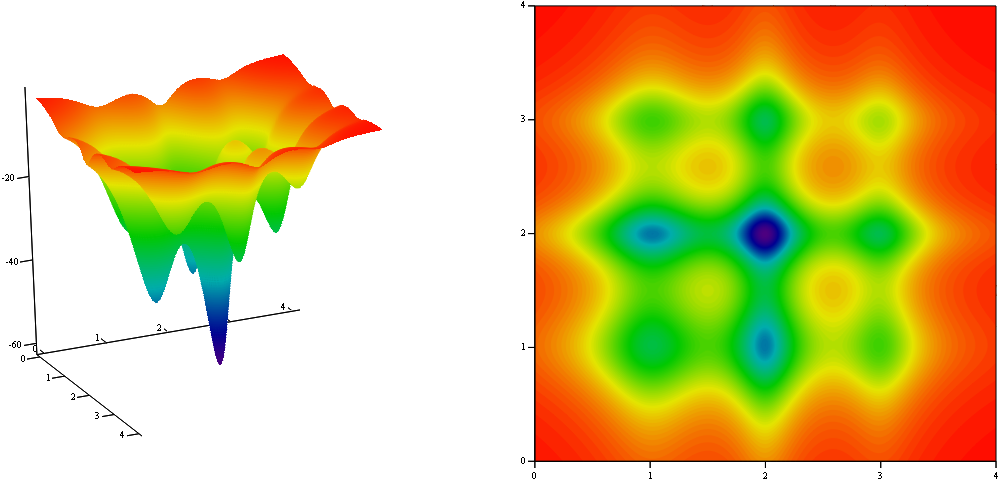
\includegraphics [scale=0.5] {MHL_TestFunction_MultiplicativePotential}
  \caption{Мультипликативная потенциальная функция} 
  \label{TestFunctions:img:MHL_TestFunction_MultiplicativePotentiale}  
\end{figure}

\subsection {Параметры для алгоритмов оптимизации}

\begin{tabularwide}
\textbf{Точность вычислений:} & $\varepsilon=0.01$. \\
\textbf{Число интервалов, на которые предполагается разбивать каждую компоненту вектора $\bar{x}$ в пределах своего изменения} (для алгоритмов дискретной оптимизации) : & $NumberOfParts_j=4095$ ($j=\overline{1,n}$). \\
\textbf{Для этого длина бинарной строки для $x_j$ координаты равна} (для алгоритмов бинарной оптимизации) : & $\left( k_2\right)_j=12$ ($j=\overline{1,n}$). \\
\end{tabularwide}

\textbf{Замечание:}  $NumberOfParts_j$ выбирается как минимальное число, удовлетворяющее соотношению:
\begin{equation*}
NumberOfParts_j=2^{\left( k_2\right)_j }-1\geq\dfrac{10\left( Right_j-Left_j\right) }{\varepsilon},\text{где } \left( k_2\right)_j \in \mathbb{N}, \left( j=\overline{1,n}\right).
\end{equation*}

\subsection {Основная задача и подзадачи}

\begin{tabularwide}
\textbf{Изменяемый параметр: } & $n$ --- размерность вещественного вектора. \\
\textbf{Значение в основной задаче:} & $n=2$.\\
\end{tabularwide}

\subsection {Нахождение ошибки оптимизации}

Пусть в результате работы алгоритма оптимизации за $N$ запусков мы нашли решения $\bar{x}_{submin}^k$ со значениями целевой функции $f\left( \bar{x}_{submin}^k\right) $ соответственно ($k=\overline{1,N}$). Используем три вида ошибок:

\textbf{Надёжность: }
\begin{equation*}
R = \dfrac{\sum_{k=1}^{N}S\left( \bar{x}_{submin}^k \right) }{N}, \text{ где}
\end{equation*}
\begin{equation*}
S\left( \bar{x}_{submin}^k \right)=\left\lbrace \begin{aligned} 1,& \text{ если } \left| \left( \bar{x}_{submin}^k \right)_j-\left( \bar{x}_{min} \right)_j\right|\leq\varepsilon, j=\overline{1,n};   \\ 0,& \text{ иначе}. \end{aligned}\right.
\end{equation*}

\textbf{Ошибка по входным параметрам:}
\begin{equation*}
E_x = \dfrac{\sum_{k=1}^{N} \left( \frac{\sqrt{\sum_{j=1}^{n}{\left( \left( \bar{x}_{submin}^k \right)_j-\left( \bar{x}_{min} \right)_j \right)}^2 }}{n} \right)  }{N}.
\end{equation*}

\textbf{Ошибка по значениям целевой функции: }
\begin{equation*}
E_f = \dfrac{\sum_{k=1}^{N} \left| f\left( \bar{x}_{submin}^k \right)-f\left( \bar{x}_{min} \right) \right|  }{N}.
\end{equation*}

\subsection {Свойства задачи}
\begin{tabularwide}
\textbf{Условной или безусловной оптимизации: } & Задача безусловной оптимизации. \\
\textbf{Одномерной или многомерной оптимизации: } & Многомерной: (двумерной). \\
\textbf{Функция унимодальная или многоэкстремальная: } & Функция многоэкстремальная. \\
\textbf{Функция стохастическая или нет: } & Функция не стохастическая. \\
\textbf{Особенности: } & Нет. \\
\end{tabularwide}

\subsection {Реализация}

Реализация функции взята из библиотеки HarrixMathLibrary в разделе <<Тестовые функции для оптимизации>>, которую можно найти по адресу \href{https://github.com/Harrix/HarrixMathLibrary} {https://github.com/Harrix/HarrixMathLibrary}.

\begin{lstlisting}[caption=Код функции MHL\_TestFunction\_MultiplicativePotential]
double MHL_TestFunction_MultiplicativePotential(double x, double y)
{
/*
Функция двух переменных: мультипликативная потенциальная функция.
Тестовая функция вещественной оптимизации.
Входные параметры:
 x - первая вещественная переменная;
 y - вторая вещественная переменная.
Возвращаемое значение:
 Значение тестовой функции в точке (x,y).
*/
double VMHL_Result;
double z1=-(1./((x-1.)*(x-1.)+0.2))-(1./(2.*(x-2.)*(x-2.)+0.15))-(1./(3.*(x-3.)*(x-3.)+0.3));
double z2=-(1./((y-1.)*(y-1.)+0.2))-(1./(2.*(y-2.)*(y-2.)+0.15))-(1./(3.*(y-3.)*(y-3.)+0.3));
VMHL_Result=-z1*z2;
return VMHL_Result;
}
\end{lstlisting}

\subsection {Ссылки}

Данная функция приводится в следующих источниках:

\begin{enumerate}
\item \cite[стр. 32]{book:Semenkin2007} ---  \href{http://files.lib.sfu-kras.ru/ebibl/umkd/22/u_lectures.pdf}{Эволюционные методы моделирования и оптимизации сложных систем}.
\end{enumerate}
\section {Функция Rana}

\subsection {Описание функции}

\begin{tabularwide}
\textbf{Идентификатор:} & MHL\_TestFunction\_Rana. \\
\textbf{Наименование:} & Функция Rana. \\
\textbf{Тип:} & Задача вещественной оптимизации. \\
\end{tabularwide}

\textbf{Формула} (целевая функция):
\begin{align}
\label{TestFunctions:eq:MHL_TestFunction_Rana}
f\left( \bar{x}\right) = & \bar{x}_1\sin\left( \sqrt{\left| \bar{x}_2+1-\bar{x}_1\right| }\right) \cos\left( \sqrt{\left| \bar{x}_2+1+\bar{x}_1\right| }\right)+  \\&+ (\bar{x}_2+1)\cos\left( \sqrt{\left| \bar{x}_2+1-\bar{x}_1\right| }\right) \sin\left( \sqrt{\left| \bar{x}_2+1+x\right| }\right), \text{ где}
\end{align}
\indent $\bar{x}\in X$, $\bar{x}_j\in \left[ Left_j; Right_j\right] $, $Left_j=-512$, $Right_j=512$, $j=\overline{1,n}$, $n=2$.

\begin{tabularwide}
\textbf{Обозначение:} &\specialcell{$\bar{x}$ --- вещественный вектор;\\$n = 2$ --- размерность вещественного вектора.}  \\
\textbf{Решаемая задача оптимизации:} & $\bar{x}_{min}= \arg \min_{\bar{x}\in X} f\left( \bar{x}\right)$.   \\
\textbf{Точка минимума:} & $\bar{x}_{min}={\left( -488.6326, 512\right)}^\mathrm{T} $.    \\
\textbf{Минимум функции:} & $f\left(\bar{x}_{min} \right) =-511.7328819$.   \\
\textbf{График:} & Рисунок \ref{TestFunctions:img:MHL_TestFunction_Ranae} нас \pageref{TestFunctions:img:MHL_TestFunction_Ranae} стр.   \\
\end{tabularwide}

\begin{figure} [h] 
  \center
  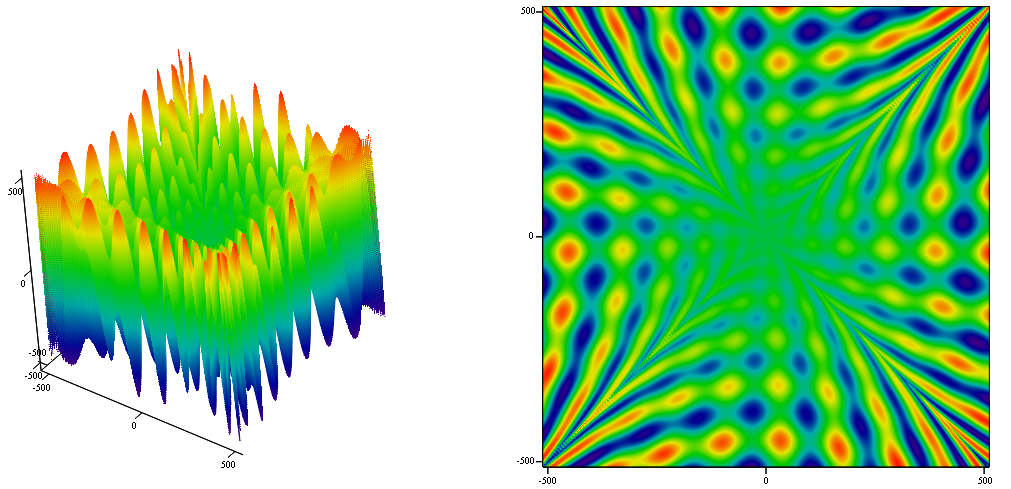
\includegraphics [scale=0.5] {MHL_TestFunction_Rana}
  \caption{Функция Rana} 
  \label{TestFunctions:img:MHL_TestFunction_Ranae}  
\end{figure}

\subsection {Параметры для алгоритмов оптимизации}

\begin{tabularwide}
\textbf{Точность вычислений:} & $\varepsilon=2.5$. \\
\textbf{Число интервалов, на которые предполагается разбивать каждую компоненту вектора $\bar{x}$ в пределах своего изменения} (для алгоритмов дискретной оптимизации) : & $NumberOfParts_j=4095$ ($j=\overline{1,n}$). \\
\textbf{Для этого длина бинарной строки для $x_j$ координаты равна} (для алгоритмов бинарной оптимизации) : & $\left( k_2\right)_j=12$ ($j=\overline{1,n}$). \\
\end{tabularwide}

\textbf{Замечание:}  $NumberOfParts_j$ выбирается как минимальное число, удовлетворяющее соотношению:
\begin{equation*}
NumberOfParts_j=2^{\left( k_2\right)_j }-1\geq\dfrac{10\left( Right_j-Left_j\right) }{\varepsilon},\text{где } \left( k_2\right)_j \in \mathbb{N}, \left( j=\overline{1,n}\right).
\end{equation*}

\subsection {Основная задача и подзадачи}

\begin{tabularwide}
\textbf{Изменяемый параметр: } & $n$ --- размерность вещественного вектора. \\
\textbf{Значение в основной задаче:} & $n=2$.\\
\end{tabularwide}

\subsection {Нахождение ошибки оптимизации}

Пусть в результате работы алгоритма оптимизации за $N$ запусков мы нашли решения $\bar{x}_{submin}^k$ со значениями целевой функции $f\left( \bar{x}_{submin}^k\right) $ соответственно ($k=\overline{1,N}$). Используем три вида ошибок:

\textbf{Надёжность: }
\begin{equation*}
R = \dfrac{\sum_{k=1}^{N}S\left( \bar{x}_{submin}^k \right) }{N}, \text{ где}
\end{equation*}
\begin{equation*}
S\left( \bar{x}_{submin}^k \right)=\left\lbrace \begin{aligned} 1,& \text{ если } \left| \left( \bar{x}_{submin}^k \right)_j-\left( \bar{x}_{min} \right)_j\right|<\varepsilon, j=\overline{1,n};   \\ 0,& \text{ иначе}. \end{aligned}\right.
\end{equation*}

\textbf{Ошибка по входным параметрам:}
\begin{equation*}
E_x = \dfrac{\sum_{k=1}^{N} \left( \frac{\sqrt{\sum_{j=1}^{n}{\left( \left( \bar{x}_{submin}^k \right)_j-\left( \bar{x}_{min} \right)_j \right)}^2 }}{n} \right)  }{N}.
\end{equation*}

\textbf{Ошибка по значениям целевой функции: }
\begin{equation*}
E_f = \dfrac{\sum_{k=1}^{N} \left| f\left( \bar{x}_{submin}^k \right)-f\left( \bar{x}_{min} \right) \right|  }{N}.
\end{equation*}

\subsection {Свойства задачи}
\begin{tabularwide}
\textbf{Условной или безусловной оптимизации: } & Задача безусловной оптимизации. \\
\textbf{Одномерной или многомерной оптимизации: } & Многомерной: (двумерной). \\
\textbf{Функция унимодальная или многоэкстремальная: } & Функция многоэкстремальная. \\
\textbf{Функция стохастическая или нет: } & Функция не стохастическая. \\
\textbf{Особенности: } & Нет. \\
\end{tabularwide}

\subsection {Реализация}

Реализация функции взята из библиотеки HarrixMathLibrary в разделе <<Тестовые функции для оптимизации>>, которую можно найти по адресу \href{https://github.com/Harrix/HarrixMathLibrary} {https://github.com/Harrix/HarrixMathLibrary}.

\begin{lstlisting}[caption=Код функции MHL\_TestFunction\_Rana]
double MHL_TestFunction_Rana(double x, double y)
{
/*
Функция двух переменных: функция Rana.
Тестовая функция вещественной оптимизации.
Входные параметры:
 x - первая вещественная переменная;
 y - вторая вещественная переменная.
Возвращаемое значение:
 Значение тестовой функции в точке (x,y).
*/
double VMHL_Result;
VMHL_Result=x*sin(sqrt(fabs(y+1.-x)))*cos(sqrt(fabs(y+1.+x))) + (y+1.)*cos(sqrt(fabs(y+1.-x)))*sin(sqrt(fabs(y+1.+x)));
return VMHL_Result;
}
\end{lstlisting}

\subsection {Ссылки}

Данная функция приводится в следующих источниках:

\begin{enumerate}
\item \cite{web:Rana} ---  \href{http://www.cs.unm.edu/~neal.holts/dga/benchmarkFunction/rana.html}{Rana}.
\item \cite{web:non_linear_continuous} ---  \href{http://www.maths.uq.edu.au/CEToolBox/node3.html}{Non-linear Continuous Multi-Extremal Optimization}.
\end{enumerate}
\section {Функция Растригина с изменением коэффициентов}

\subsection {Описание функции}

\begin{tabularwide}
\textbf{Идентификатор:} & MHL\_TestFunction\_RastriginWithChange. \\
\textbf{Наименование:} & Функция Растригина с изменением коэффициентов. \\
\textbf{Тип:} & Задача вещественной оптимизации. \\
\end{tabularwide}

\textbf{Формула} (целевая функция):
\begin{equation}
\label{TestFunctions:eq:MHL_TestFunction_RastriginWithChange}
f\left( \bar{x}\right) =0.1\bar{x}_1^2+0.1\bar{x}_2^2-4\cos\left( 0.8\bar{x}_1\right) -4\cos\left( 0.8\bar{x}_2\right) +8, \text{ где}
\end{equation}
\indent $\bar{x}\in X$, $\bar{x}_j\in \left[ Left_j; Right_j\right] $, $Left_j=-16$, $Right_j=16$, $j=\overline{1,n}$, $n=2$.

\begin{tabularwide}
\textbf{Обозначение:} &\specialcell{$\bar{x}$ --- вещественный вектор;\\$n = 2$ --- размерность вещественного вектора.}  \\
\textbf{Решаемая задача оптимизации:} & $\bar{x}_{max}= \arg \max_{\bar{x}\in X} f\left( \bar{x}\right)$.   \\
\textbf{Точка максимума:} & $\bar{x}_{max}={\left( 0, 0\right)}^\mathrm{T} $, то есть $\left(\bar{x}_{max} \right)_j=0$ ($j=\overline{1,n}$).    \\
\textbf{Максимум функции:} & $f\left(\bar{x}_{max} \right) =0$.   \\
\textbf{График:} & Рисунок \ref{TestFunctions:img:MHL_TestFunction_RastriginWithChangee} нас \pageref{TestFunctions:img:MHL_TestFunction_RastriginWithChangee} стр.   \\
\end{tabularwide}

\begin{figure} [h] 
  \center
  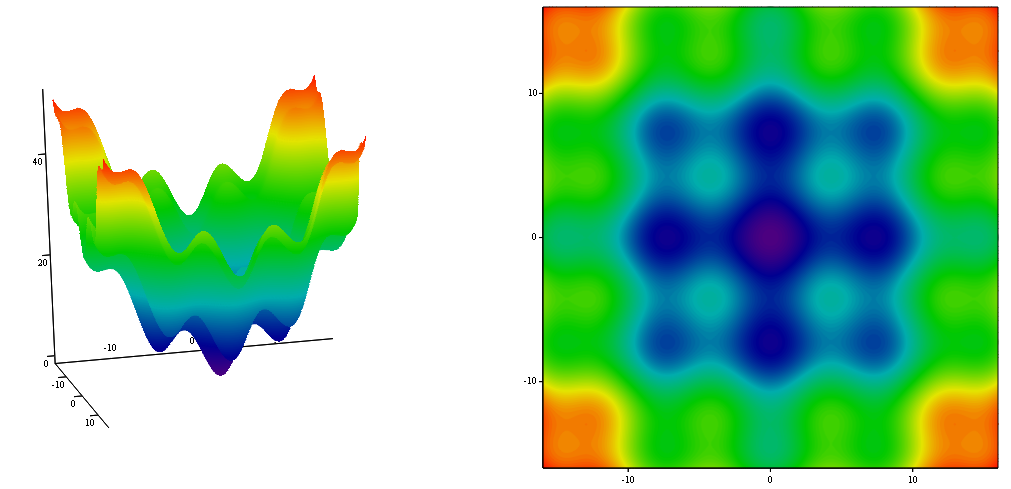
\includegraphics [scale=0.5] {MHL_TestFunction_RastriginWithChange}
  \caption{Функция Растригина с изменением коэффициентов} 
  \label{TestFunctions:img:MHL_TestFunction_RastriginWithChangee}  
\end{figure}

\subsection {Параметры для алгоритмов оптимизации}

\begin{tabularwide}
\textbf{Точность вычислений:} & $\varepsilon=0.08$. \\
\textbf{Число интервалов, на которые предполагается разбивать каждую компоненту вектора $\bar{x}$ в пределах своего изменения} (для алгоритмов дискретной оптимизации) : & $NumberOfParts_j=4095$ ($j=\overline{1,n}$). \\
\textbf{Для этого длина бинарной строки для $x_j$ координаты равна} (для алгоритмов бинарной оптимизации) : & $\left( k_2\right)_j=12$ ($j=\overline{1,n}$). \\
\end{tabularwide}

\textbf{Замечание:}  $NumberOfParts_j$ выбирается как минимальное число, удовлетворяющее соотношению:
\begin{equation*}
NumberOfParts_j=2^{\left( k_2\right)_j }-1\geq\dfrac{10\left( Right_j-Left_j\right) }{\varepsilon},\text{где } \left( k_2\right)_j \in \mathbb{N}, \left( j=\overline{1,n}\right).
\end{equation*}

\subsection {Основная задача и подзадачи}

\begin{tabularwide}
\textbf{Изменяемый параметр: } & $n$ --- размерность вещественного вектора. \\
\textbf{Значение в основной задаче:} & $n=2$.\\
\end{tabularwide}

\subsection {Нахождение ошибки оптимизации}

Пусть в результате работы алгоритма оптимизации за $N$ запусков мы нашли решения $\bar{x}_{submin}^k$ со значениями целевой функции $f\left( \bar{x}_{submin}^k\right) $ соответственно ($k=\overline{1,N}$). Используем три вида ошибок:

\textbf{Надёжность: }
\begin{equation*}
R = \dfrac{\sum_{k=1}^{N}S\left( \bar{x}_{submin}^k \right) }{N}, \text{ где}
\end{equation*}
\begin{equation*}
S\left( \bar{x}_{submin}^k \right)=\left\lbrace \begin{aligned} 1,& \text{ если } \left| \left( \bar{x}_{submin}^k \right)_j-\left( \bar{x}_{min} \right)_j\right|<\varepsilon, j=\overline{1,n};   \\ 0,& \text{ иначе}. \end{aligned}\right.
\end{equation*}

\textbf{Ошибка по входным параметрам:}
\begin{equation*}
E_x = \dfrac{\sum_{k=1}^{N} \left( \frac{\sqrt{\sum_{j=1}^{n}{\left( \left( \bar{x}_{submin}^k \right)_j-\left( \bar{x}_{min} \right)_j \right)}^2 }}{n} \right)  }{N}.
\end{equation*}

\textbf{Ошибка по значениям целевой функции: }
\begin{equation*}
E_f = \dfrac{\sum_{k=1}^{N} \left| f\left( \bar{x}_{submin}^k \right)-f\left( \bar{x}_{min} \right) \right|  }{N}.
\end{equation*}

\subsection {Свойства задачи}
\begin{tabularwide}
\textbf{Условной или безусловной оптимизации: } & Задача безусловной оптимизации. \\
\textbf{Одномерной или многомерной оптимизации: } & Многомерной: (двумерной). \\
\textbf{Функция унимодальная или многоэкстремальная: } & Функция многоэкстремальная. \\
\textbf{Функция стохастическая или нет: } & Функция не стохастическая. \\
\textbf{Особенности: } & Нет. \\
\end{tabularwide}

\subsection {Реализация}

Реализация функции взята из библиотеки HarrixMathLibrary в разделе <<Тестовые функции для оптимизации>>, которую можно найти по адресу \href{https://github.com/Harrix/HarrixMathLibrary} {https://github.com/Harrix/HarrixMathLibrary}.

\begin{lstlisting}[caption=Код функции MHL\_TestFunction\_RastriginWithChange]
double MHL_TestFunction_RastriginWithChange(double x, double y)
{
/*
Функция двух переменных: функция Растригина с изменением коэффициентов.
Тестовая функция вещественной оптимизации.
Входные параметры:
 x - первая вещественная переменная;
 y - вторая вещественная переменная.
Возвращаемое значение:
 Значение тестовой функции в точке (x,y).
*/
double VMHL_Result;

VMHL_Result=0.1*x*x+0.1*y*y-4.*cos(0.8*x)-4.*cos(0.8*y)+8.;

return VMHL_Result;
}
\end{lstlisting}

\subsection {Ссылки}


Данная функция приводится в следующих источниках:

\begin{enumerate}
\item \cite[стр. 27]{book:Semenkin2007} ---  \href{http://files.lib.sfu-kras.ru/ebibl/umkd/22/u_lectures.pdf}{Эволюционные методы моделирования и оптимизации сложных систем}.
\end{enumerate}
\section {Функция Растригина овражная с поворотом осей}
\label{TestFunctions:section:MHL_TestFunction_RastriginWithTurning}
\subsection {Описание функции}

\begin{tabularwide}
\textbf{Идентификатор:} & MHL\_TestFunction\_RastriginWithTurning. \\
\textbf{Наименование:} & Функция Растригина овражная с поворотом осей. \\
\textbf{Тип:} & Задача вещественной оптимизации. \\
\end{tabularwide}

\textbf{Формула} (целевая функция):
\begin{align}
\label{TestFunctions:eq:MHL_TestFunction_RastriginWithTurning}
f\left( \bar{x}\right) =&{\left( 0.1 K_{\bar{x}_1}A\left( \bar{x}_1,\bar{x}_2\right) \right) }^2+{\left( 0.1 K_{\bar{x}_2}B\left( \bar{x}_1,\bar{x}_2\right) \right) }^2-
\\&-4\cos\left( 0.8K_{\bar{x}_1}A\left( \bar{x}_1,\bar{x}_2\right)\right) -4\cos\left( 0.8K_{\bar{x}_2}B\left( \bar{x}_1,\bar{x}_2\right)\right) +8, \text{ где}\nonumber
\\&A\left( \bar{x}_1,\bar{x}_2\right)= \bar{x}_1\cos\left( \alpha\right) -\bar{x}_2\sin\left( \alpha\right),\nonumber
\\&B\left( \bar{x}_1,\bar{x}_2\right)= \bar{x}_1\sin\left( \alpha\right) +\bar{x}_2\cos\left( \alpha\right),\nonumber
\end{align}
\indent $\bar{x}\in X$, $\bar{x}_j\in \left[ Left_j; Right_j\right] $, $Left_j=-16$, $Right_j=16$, $j=\overline{1,n}$, $n=2$, $ K_{\bar{x}_1}=1.5 $, $ K_{\bar{x}_2}= 0.8$, $\alpha=\frac{\pi}{2}  $.

\begin{tabularwide}
\textbf{Обозначение:} &\specialcell{$\bar{x}$ --- вещественный вектор;\\$n = 2$ --- размерность вещественного вектора.}  \\
\textbf{Решаемая задача оптимизации:} & $\bar{x}_{max}= \arg \max_{\bar{x}\in X} f\left( \bar{x}\right)$.   \\
\textbf{Точка максимума:} & $\bar{x}_{max}={\left( 0, 0\right)}^\mathrm{T} $, то есть $\left(\bar{x}_{max} \right)_j=0$ ($j=\overline{1,n}$).    \\
\textbf{Максимум функции:} & $f\left(\bar{x}_{max} \right) =0$.   \\
\textbf{График:} & Рисунок \ref{TestFunctions:img:MHL_TestFunction_RastriginWithTurninge} нас \pageref{TestFunctions:img:MHL_TestFunction_RastriginWithTurninge} стр.   \\
\end{tabularwide}

\begin{figure} [h] 
  \center
  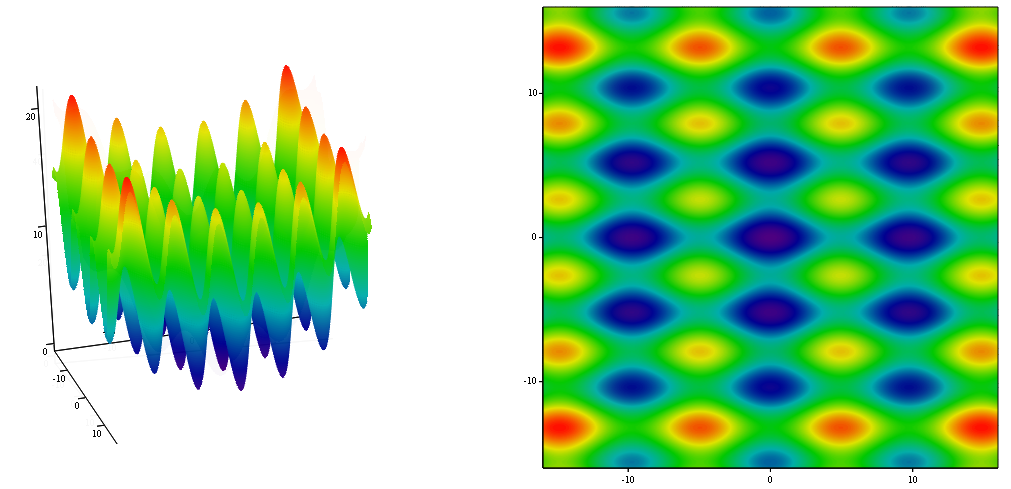
\includegraphics [scale=0.5] {MHL_TestFunction_RastriginWithTurning}
  \caption{Функция Растригина овражная с поворотом осей} 
  \label{TestFunctions:img:MHL_TestFunction_RastriginWithTurninge}  
\end{figure}

\subsection {Параметры для алгоритмов оптимизации}

\begin{tabularwide}
\textbf{Точность вычислений:} & $\varepsilon=0.08$. \\
\textbf{Число интервалов, на которые предполагается разбивать каждую компоненту вектора $\bar{x}$ в пределах своего изменения} (для алгоритмов дискретной оптимизации) : & $NumberOfParts_j=4095$ ($j=\overline{1,n}$). \\
\textbf{Для этого длина бинарной строки для $x_j$ координаты равна} (для алгоритмов бинарной оптимизации) : & $\left( k_2\right)_j=12$ ($j=\overline{1,n}$). \\
\end{tabularwide}

\textbf{Замечание:}  $NumberOfParts_j$ выбирается как минимальное число, удовлетворяющее соотношению:
\begin{equation*}
NumberOfParts_j=2^{\left( k_2\right)_j }-1\geq\dfrac{10\left( Right_j-Left_j\right) }{\varepsilon},\text{где } \left( k_2\right)_j \in \mathbb{N}, \left( j=\overline{1,n}\right).
\end{equation*}

\subsection {Основная задача и подзадачи}

\begin{tabularwide}
\textbf{Изменяемый параметр: } & $n$ --- размерность вещественного вектора. \\
\textbf{Значение в основной задаче:} & $n=2$.\\
\end{tabularwide}

\subsection {Нахождение ошибки оптимизации}

Пусть в результате работы алгоритма оптимизации за $N$ запусков мы нашли решения $\bar{x}_{submin}^k$ со значениями целевой функции $f\left( \bar{x}_{submin}^k\right) $ соответственно ($k=\overline{1,N}$). Используем три вида ошибок:

\textbf{Надёжность: }
\begin{equation*}
R = \dfrac{\sum_{k=1}^{N}S\left( \bar{x}_{submin}^k \right) }{N}, \text{ где}
\end{equation*}
\begin{equation*}
S\left( \bar{x}_{submin}^k \right)=\left\lbrace \begin{aligned} 1,& \text{ если } \left| \left( \bar{x}_{submin}^k \right)_j-\left( \bar{x}_{min} \right)_j\right|<\varepsilon, j=\overline{1,n};   \\ 0,& \text{ иначе}. \end{aligned}\right.
\end{equation*}

\textbf{Ошибка по входным параметрам:}
\begin{equation*}
E_x = \dfrac{\sum_{k=1}^{N} \left( \frac{\sqrt{\sum_{j=1}^{n}{\left( \left( \bar{x}_{submin}^k \right)_j-\left( \bar{x}_{min} \right)_j \right)}^2 }}{n} \right)  }{N}.
\end{equation*}

\textbf{Ошибка по значениям целевой функции: }
\begin{equation*}
E_f = \dfrac{\sum_{k=1}^{N} \left| f\left( \bar{x}_{submin}^k \right)-f\left( \bar{x}_{min} \right) \right|  }{N}.
\end{equation*}

\subsection {Свойства задачи}
\begin{tabularwide}
\textbf{Условной или безусловной оптимизации: } & Задача безусловной оптимизации. \\
\textbf{Одномерной или многомерной оптимизации: } & Многомерной: (двумерной). \\
\textbf{Функция унимодальная или многоэкстремальная: } & Функция многоэкстремальная. \\
\textbf{Функция стохастическая или нет: } & Функция не стохастическая. \\
\textbf{Особенности: } & Нет. \\
\end{tabularwide}

\subsection {Реализация}

Реализация функции взята из библиотеки HarrixMathLibrary в разделе <<Тестовые функции для оптимизации>>, которую можно найти по адресу \href{https://github.com/Harrix/HarrixMathLibrary} {https://github.com/Harrix/HarrixMathLibrary}.

\begin{lstlisting}[caption=Код функции MHL\_TestFunction\_RastriginWithTurning]
double MHL_TestFunction_RastriginWithTurning(double x, double y)
{
/*
Функция двух переменных: функция Растригина овражная с поворотом осей.
Тестовая функция вещественной оптимизации.
Входные параметры:
 x - первая вещественная переменная;
 y - вторая вещественная переменная.
Возвращаемое значение:
 Значение тестовой функции в точке (x,y).
*/
double VMHL_Result;

double alpha=MHL_PI_2;
double kx=1.5;
double ky=0.8;

double A,B;
A=x*cos(alpha)-y*sin(alpha);
B=x*sin(alpha)+y*cos(alpha);

VMHL_Result=(0.1*kx*A)*(0.1*kx*A)+(0.1*ky*B)*(0.1*ky*B)-4.*cos(0.8*kx*A)-4.*cos(0.8*ky*B)+8.;

return VMHL_Result;
}
\end{lstlisting}

\subsection {Ссылки}


Данная функция приводится в следующих источниках:

\begin{enumerate}
\item \cite[стр. 28]{book:Semenkin2007} ---  \href{http://files.lib.sfu-kras.ru/ebibl/umkd/22/u_lectures.pdf}{Эволюционные методы моделирования и оптимизации сложных систем}.
\end{enumerate}
\section {Функция ReverseGriewank}

\subsection {Описание функции}

\begin{tabularwide}
\textbf{Идентификатор:} & MHL\_TestFunction\_ReverseGriewank. \\
\textbf{Наименование:} & Функция ReverseGriewank. \\
\textbf{Тип:} & Задача вещественной оптимизации. \\
\end{tabularwide}

\textbf{Формула} (целевая функция):
\begin{equation}
\label{TestFunctions:eq:MHL_ReverseGriewank}
f\left( \bar{x}\right) = \dfrac{1}{\dfrac{\bar{x}_1^2+\bar{x}_2^2}{200}-cos\left( \bar{x}_0\right)cos\left( \dfrac{\bar{x}_2}{\sqrt{2}}\right)+2  }, \text{ где}
\end{equation}
\indent $\bar{x}\in X$, $\bar{x}_j\in \left[ Left_j; Right_j\right] $, $Left_j=-10$, $Right_j=10$, $j=\overline{1,n}$, $n=2$.

\begin{tabularwide}
\textbf{Обозначение:} &\specialcell{$\bar{x}$ --- вещественный вектор;\\$n = 2$ --- размерность вещественного вектора.}  \\
\textbf{Решаемая задача оптимизации:} & $\bar{x}_{max}= \arg \max_{\bar{x}\in X} f\left( \bar{x}\right)$.   \\
\textbf{Точка максимума:} & $\bar{x}_{max}={\left( 0, 0\right)}^\mathrm{T} $, то есть $\left(\bar{x}_{max} \right)_j=0$ ($j=\overline{1,n}$).    \\
\textbf{Максимум функции:} & $f\left(\bar{x}_{max} \right) =1$.   \\
\textbf{График:} & Рисунок \ref{TestFunctions:img:MHL_TestFunction_ReverseGriewanke} нас \pageref{TestFunctions:img:MHL_TestFunction_ReverseGriewanke} стр.   \\
\end{tabularwide}

\begin{figure} [h] 
  \center
  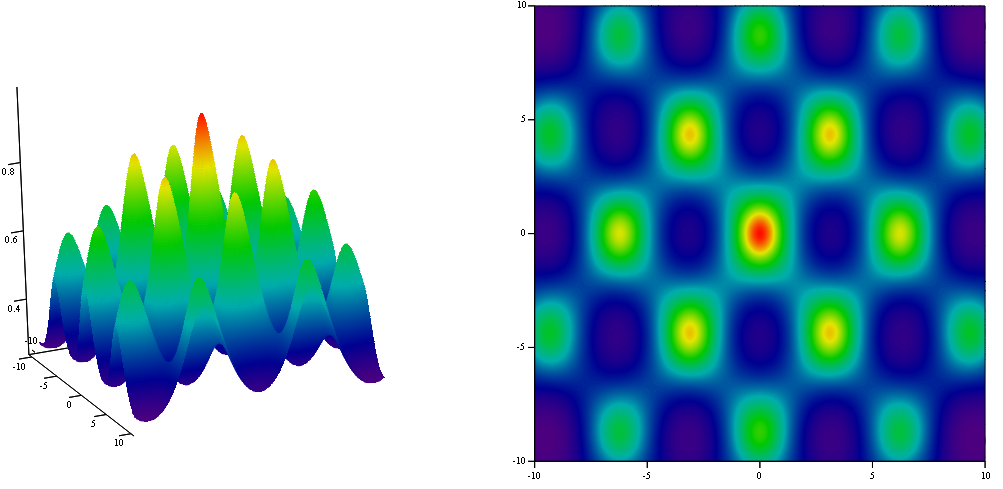
\includegraphics [scale=0.5] {MHL_TestFunction_ReverseGriewank}
  \caption{Функция ReverseGriewank} 
  \label{TestFunctions:img:MHL_TestFunction_ReverseGriewanke}  
\end{figure}

\subsection {Параметры для алгоритмов оптимизации}

\begin{tabularwide}
\textbf{Точность вычислений:} & $\varepsilon=0.05$. \\
\textbf{Число интервалов, на которые предполагается разбивать каждую компоненту вектора $\bar{x}$ в пределах своего изменения} (для алгоритмов дискретной оптимизации) : & $NumberOfParts_j=4095$ ($j=\overline{1,n}$). \\
\textbf{Для этого длина бинарной строки для $x_j$ координаты равна} (для алгоритмов бинарной оптимизации) : & $\left( k_2\right)_j=12$ ($j=\overline{1,n}$). \\
\end{tabularwide}

\textbf{Замечание:}  $NumberOfParts_j$ выбирается как минимальное число, удовлетворяющее соотношению:
\begin{equation*}
NumberOfParts_j=2^{\left( k_2\right)_j }-1\geq\dfrac{10\left( Right_j-Left_j\right) }{\varepsilon},\text{где } \left( k_2\right)_j \in \mathbb{N}, \left( j=\overline{1,n}\right).
\end{equation*}

\subsection {Основная задача и подзадачи}

\begin{tabularwide}
\textbf{Изменяемый параметр: } & $n$ --- размерность вещественного вектора. \\
\textbf{Значение в основной задаче:} & $n=2$.\\
\end{tabularwide}

\subsection {Нахождение ошибки оптимизации}

Пусть в результате работы алгоритма оптимизации за $N$ запусков мы нашли решения $\bar{x}_{submin}^k$ со значениями целевой функции $f\left( \bar{x}_{submin}^k\right) $ соответственно ($k=\overline{1,N}$). Используем три вида ошибок:

\textbf{Надёжность: }
\begin{equation*}
R = \dfrac{\sum_{k=1}^{N}S\left( \bar{x}_{submin}^k \right) }{N}, \text{ где}
\end{equation*}
\begin{equation*}
S\left( \bar{x}_{submin}^k \right)=\left\lbrace \begin{aligned} 1,& \text{ если } \left| \left( \bar{x}_{submin}^k \right)_j-\left( \bar{x}_{min} \right)_j\right|<\varepsilon, j=\overline{1,n};   \\ 0,& \text{ иначе}. \end{aligned}\right.
\end{equation*}

\textbf{Ошибка по входным параметрам:}
\begin{equation*}
E_x = \dfrac{\sum_{k=1}^{N} \left( \frac{\sqrt{\sum_{j=1}^{n}{\left( \left( \bar{x}_{submin}^k \right)_j-\left( \bar{x}_{min} \right)_j \right)}^2 }}{n} \right)  }{N}.
\end{equation*}

\textbf{Ошибка по значениям целевой функции: }
\begin{equation*}
E_f = \dfrac{\sum_{k=1}^{N} \left| f\left( \bar{x}_{submin}^k \right)-f\left( \bar{x}_{min} \right) \right|  }{N}.
\end{equation*}

\subsection {Свойства задачи}
\begin{tabularwide}
\textbf{Условной или безусловной оптимизации: } & Задача безусловной оптимизации. \\
\textbf{Одномерной или многомерной оптимизации: } & Многомерной: (двумерной). \\
\textbf{Функция унимодальная или многоэкстремальная: } & Функция многоэкстремальная. \\
\textbf{Функция стохастическая или нет: } & Функция не стохастическая. \\
\textbf{Особенности: } & Нет. \\
\end{tabularwide}

\subsection {Реализация}

Реализация функции взята из библиотеки HarrixMathLibrary в разделе <<Тестовые функции для оптимизации>>, которую можно найти по адресу \href{https://github.com/Harrix/HarrixMathLibrary} {https://github.com/Harrix/HarrixMathLibrary}.

\begin{lstlisting}[caption=Код функции MHL\_TestFunction\_ReverseGriewank]
double MHL_TestFunction_ReverseGriewank(double x, double y)
{
/*
Функция двух переменных: функция ReverseGriewank.
Тестовая функция вещественной оптимизации.
Входные параметры:
 x - первая вещественная переменная;
 y - вторая вещественная переменная.
Возвращаемое значение:
 Значение тестовой функции в точке (x,y).
*/
double VMHL_Result;

VMHL_Result = 1./((x*x+y*y)/200.-cos(x)*cos(y/sqrt(2.))+2.);

return VMHL_Result;
}
\end{lstlisting}

\subsection {Ссылки}

Так и не смог найти нормальный источник для этой функции. По внешнему виду похожа на функцию Гриванка, которую возвели в $-1$ степень. Откуда-то у меня находится со студенческих времен.
\section {Функция <<Лисьи норы>> Шекеля}
\label{TestFunctions:section:MHL_TestFunction_ShekelsFoxholes}
\subsection {Описание функции}

\begin{tabularwide}
\textbf{Идентификатор:} & MHL\_TestFunction\_ShekelsFoxholes. \\
\textbf{Наименование:} & Функция <<Лисьи норы>> Шекеля. \\
\textbf{Тип:} & Задача вещественной оптимизации. \\
\end{tabularwide}

\textbf{Формула} (целевая функция):
\begin{equation}
\label{TestFunctions:eq:MHL_TestFunction_ShekelsFoxholes}
f\left( \bar{x}\right) = \dfrac{1}{\dfrac{1}{K}+\sum_{j=1}^{25}\dfrac{1}{j+\left( \bar{x}_1-A_{1,j}\right)^6+ \left( \bar{x}_2-A_{2,j}\right)^6}}, \text{ где}
\end{equation}
\indent $\bar{x}\in X$, $\bar{x}_j\in \left[ Left_j; Right_j\right] $, $Left_j=-50$, $Right_j=50$, $j=\overline{1,n}$, $n=2$, $K=500$,
\begin{equation*}
A =  \bigl(\begin{smallmatrix}
-32 & -16 & 0 & 16 & 32 & -32 & -16 & 0 & 16 & 32 & -32 & -16 & 0 & 16 & 32 & -32 & -16 & 0 & 16 & 32 & -32 & -16 & 0 & 16 & 32\\
-32 & -32 & -32 & -32 & -32 & -16 & -16 & -16 & -16 & -16 & 0 & 0 & 0 & 0 & 0 & 16 & 16 & 16 & 16 & 16 & 32 & 32 & 32 & 32 & 32
\end{smallmatrix}\bigr).
\end{equation*}

\begin{tabularwide}
\textbf{Обозначение:} &\specialcell{$\bar{x}$ --- вещественный вектор;\\$n = 2$ --- размерность вещественного вектора.}  \\
\textbf{Решаемая задача оптимизации:} & $\bar{x}_{min}= \arg \min_{\bar{x}\in X} f\left( \bar{x}\right)$.   \\
\textbf{Точка минимума:} & $\bar{x}_{min}={\left( -32, -32\right)}^\mathrm{T} $, то есть $\left(\bar{x}_{min} \right)_j=-32$ ($j=\overline{1,n}$).    \\
\textbf{Минимум функции:} & $f\left(\bar{x}_{min} \right) =0.99800384$.   \\
\textbf{График:} & Рисунок \ref{TestFunctions:img:MHL_TestFunction_ShekelsFoxholese} нас \pageref{TestFunctions:img:MHL_TestFunction_ShekelsFoxholese} стр.   \\
\end{tabularwide}

\begin{figure} [h] 
  \center
  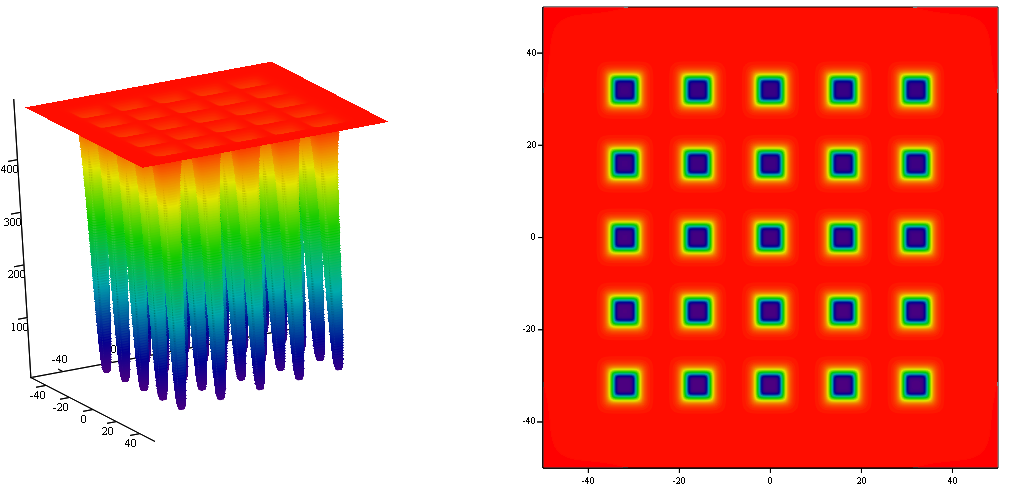
\includegraphics [scale=0.5] {MHL_TestFunction_ShekelsFoxholes}
  \caption{Функция <<Лисьи норы>> Шекеля} 
  \label{TestFunctions:img:MHL_TestFunction_ShekelsFoxholese}  
\end{figure}

\subsection {Параметры для алгоритмов оптимизации}

\begin{tabularwide}
\textbf{Точность вычислений:} & $\varepsilon=0.25$. \\
\textbf{Число интервалов, на которые предполагается разбивать каждую компоненту вектора $\bar{x}$ в пределах своего изменения} (для алгоритмов дискретной оптимизации) : & $NumberOfParts_j=4095$ ($j=\overline{1,n}$). \\
\textbf{Для этого длина бинарной строки для $x_j$ координаты равна} (для алгоритмов бинарной оптимизации) : & $\left( k_2\right)_j=12$ ($j=\overline{1,n}$). \\
\end{tabularwide}

\textbf{Замечание:}  $NumberOfParts_j$ выбирается как минимальное число, удовлетворяющее соотношению:
\begin{equation*}
NumberOfParts_j=2^{\left( k_2\right)_j }-1\geq\dfrac{10\left( Right_j-Left_j\right) }{\varepsilon},\text{где } \left( k_2\right)_j \in \mathbb{N}, \left( j=\overline{1,n}\right).
\end{equation*}

\subsection {Основная задача и подзадачи}

\begin{tabularwide}
\textbf{Изменяемый параметр: } & $n$ --- размерность вещественного вектора. \\
\textbf{Значение в основной задаче:} & $n=2$.\\
\end{tabularwide}

\subsection {Нахождение ошибки оптимизации}

Пусть в результате работы алгоритма оптимизации за $N$ запусков мы нашли решения $\bar{x}_{submin}^k$ со значениями целевой функции $f\left( \bar{x}_{submin}^k\right) $ соответственно ($k=\overline{1,N}$). Используем три вида ошибок:

\textbf{Надёжность: }
\begin{equation*}
R = \dfrac{\sum_{k=1}^{N}S\left( \bar{x}_{submin}^k \right) }{N}, \text{ где}
\end{equation*}
\begin{equation*}
S\left( \bar{x}_{submin}^k \right)=\left\lbrace \begin{aligned} 1,& \text{ если } \left| \left( \bar{x}_{submin}^k \right)_j-\left( \bar{x}_{min} \right)_j\right|<\varepsilon, j=\overline{1,n};   \\ 0,& \text{ иначе}. \end{aligned}\right.
\end{equation*}

\textbf{Ошибка по входным параметрам:}
\begin{equation*}
E_x = \dfrac{\sum_{k=1}^{N} \left( \frac{\sqrt{\sum_{j=1}^{n}{\left( \left( \bar{x}_{submin}^k \right)_j-\left( \bar{x}_{min} \right)_j \right)}^2 }}{n} \right)  }{N}.
\end{equation*}

\textbf{Ошибка по значениям целевой функции: }
\begin{equation*}
E_f = \dfrac{\sum_{k=1}^{N} \left| f\left( \bar{x}_{submin}^k \right)-f\left( \bar{x}_{min} \right) \right|  }{N}.
\end{equation*}

\subsection {Свойства задачи}
\begin{tabularwide}
\textbf{Условной или безусловной оптимизации: } & Задача безусловной оптимизации. \\
\textbf{Одномерной или многомерной оптимизации: } & Многомерной: (двумерной). \\
\textbf{Функция унимодальная или многоэкстремальная: } & Функция многоэкстремальная. \\
\textbf{Функция стохастическая или нет: } & Функция не стохастическая. \\
\textbf{Особенности: } & Глобальный минимум слабо отличается от локальных. Из локальных минимумов алгоритмам обычно сложно выбраться.\\
\end{tabularwide}

\subsection {Реализация}

Реализация функции взята из библиотеки HarrixMathLibrary в разделе <<Тестовые функции для оптимизации>>, которую можно найти по адресу \href{https://github.com/Harrix/HarrixMathLibrary} {https://github.com/Harrix/HarrixMathLibrary}.

\begin{lstlisting}[caption=Код функции MHL\_TestFunction\_ShekelsFoxholes]
double MHL_TestFunction_ShekelsFoxholes(double x, double y)
{
/*
Функция двух переменных: функция "Лисьи норы" Шекеля.
Тестовая функция вещественной оптимизации.
Входные параметры:
 x - первая вещественная переменная;
 y - вторая вещественная переменная.
Возвращаемое значение:
 Значение тестовой функции в точке (x,y).
*/
double VMHL_Result;
double K=500.;
double f1,f2;
int j,k;
int a[2][25];

a[0][0]=-32;
a[0][1]=-16;
a[0][2]=0;
a[0][3]=16;
a[0][4]=32;
a[0][5]=-32;
a[0][6]=-16;
a[0][7]=0;
a[0][8]=16;
a[0][9]=32;
a[0][10]=-32;
a[0][11]=-16;
a[0][12]=0;
a[0][13]=16;
a[0][14]=32;
a[0][15]=-32;
a[0][16]=-16;
a[0][17]=0;
a[0][18]=16;
a[0][19]=32;
a[0][20]=-32;
a[0][21]=-16;
a[0][22]=0;
a[0][23]=16;
a[0][24]=32;

a[1][0]=-32;
a[1][1]=-32;
a[1][2]=-32;
a[1][3]=-32;
a[1][4]=-32;
a[1][5]=-16;
a[1][6]=-16;
a[1][7]=-16;
a[1][8]=-16;
a[1][9]=-16;
a[1][10]=0;
a[1][11]=0;
a[1][12]=0;
a[1][13]=0;
a[1][14]=0;
a[1][15]=16;
a[1][16]=16;
a[1][17]=16;
a[1][18]=16;
a[1][19]=16;
a[1][20]=32;
a[1][21]=32;
a[1][22]=32;
a[1][23]=32;
a[1][24]=32;

VMHL_Result=1./K;
for (j=0;j<25;j++)
 {
 f1=1;
 for (k=0;k<6;k++) f1=f1*(x-a[0][j]);
 f2=1;
 for (k=0;k<6;k++) f2=f2*(y-a[1][j]);
 VMHL_Result+=1./(j+1.+f1+f2);
 }
 
VMHL_Result=1./VMHL_Result;

return VMHL_Result;
}
\end{lstlisting}

\subsection {Ссылки}

Данная функция приводится в следующих источниках:

\begin{enumerate}
\item \cite[стр. 34]{book:Semenkin2007} ---  \href{http://files.lib.sfu-kras.ru/ebibl/umkd/22/u_lectures.pdf}{Эволюционные методы моделирования и оптимизации сложных систем}.
\item \cite[стр. 729]{book:huang2006international} ---  \href{http://books.google.ru/books?id=7sH4RsXYu7cC}{International Conference on Intelligent Computing: Intelligent computing}.
\end{enumerate}
\section {Функция Сомбреро}
\label{TestFunctions:section:MHL_TestFunction_Sombrero}
\subsection {Описание функции}

\begin{tabularwide}
\textbf{Идентификатор:} & MHL\_TestFunction\_Sombrero. \\
\textbf{Наименование:} & Функция Сомбреро. \\
\textbf{Тип:} & Задача вещественной оптимизации. \\
\end{tabularwide}

\textbf{Формула} (целевая функция):
\begin{equation}
\label{TestFunctions:eq:MHL_TestFunction_Sombrero}
f\left( \bar{x}\right) =\dfrac{1-{sin\left( \sqrt{\bar{x}_1^2+\bar{x}_2^2}\right)}^2 }{1+0.001\left(\bar{x}_1^2+\bar{x}_2^2 \right) }, \text{ где}
\end{equation}
\indent $\bar{x}\in X$, $\bar{x}_j\in \left[ Left_j; Right_j\right] $, $Left_j=-10$, $Right_j=10$, $j=\overline{1,n}$, $n=2$.

\begin{tabularwide}
\textbf{Обозначение:} &\specialcell{$\bar{x}$ --- вещественный вектор;\\$n = 2$ --- размерность вещественного вектора.}  \\
\textbf{Решаемая задача оптимизации:} & $\bar{x}_{max}= \arg \max_{\bar{x}\in X} f\left( \bar{x}\right)$.   \\
\textbf{Точка максимума:} & $\bar{x}_{max}={\left( 0, 0\right)}^\mathrm{T} $, то есть $\left(\bar{x}_{max} \right)_j=0$ ($j=\overline{1,n}$).    \\
\textbf{Максимум функции:} & $f\left(\bar{x}_{max} \right) =1$.   \\
\textbf{График:} & Рисунок \ref{TestFunctions:img:MHL_TestFunction_Sombreroe} нас \pageref{TestFunctions:img:MHL_TestFunction_Sombreroe} стр.   \\
\end{tabularwide}

\begin{figure} [h] 
  \center
  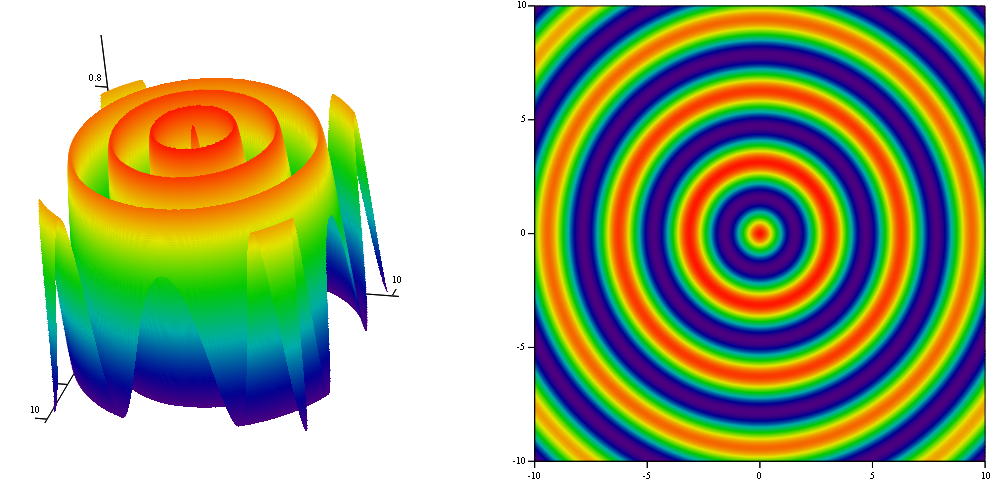
\includegraphics [scale=0.5] {MHL_TestFunction_Sombrero}
  \caption{Функция Сомбреро} 
  \label{TestFunctions:img:MHL_TestFunction_Sombreroe}  
\end{figure}

\subsection {Параметры для алгоритмов оптимизации}

\begin{tabularwide}
\textbf{Точность вычислений:} & $\varepsilon=0.05$. \\
\textbf{Число интервалов, на которые предполагается разбивать каждую компоненту вектора $\bar{x}$ в пределах своего изменения} (для алгоритмов дискретной оптимизации) : & $NumberOfParts_j=4095$ ($j=\overline{1,n}$). \\
\textbf{Для этого длина бинарной строки для $x_j$ координаты равна} (для алгоритмов бинарной оптимизации) : & $\left( k_2\right)_j=12$ ($j=\overline{1,n}$). \\
\end{tabularwide}

\textbf{Замечание:}  $NumberOfParts_j$ выбирается как минимальное число, удовлетворяющее соотношению:
\begin{equation*}
NumberOfParts_j=2^{\left( k_2\right)_j }-1\geq\dfrac{10\left( Right_j-Left_j\right) }{\varepsilon},\text{где } \left( k_2\right)_j \in \mathbb{N}, \left( j=\overline{1,n}\right).
\end{equation*}

\subsection {Основная задача и подзадачи}

\begin{tabularwide}
\textbf{Изменяемый параметр: } & $n$ --- размерность вещественного вектора. \\
\textbf{Значение в основной задаче:} & $n=2$.\\
\end{tabularwide}

\subsection {Нахождение ошибки оптимизации}

Пусть в результате работы алгоритма оптимизации за $N$ запусков мы нашли решения $\bar{x}_{submax}^k$ со значениями целевой функции $f\left( \bar{x}_{submax}^k\right) $ соответственно ($k=\overline{1,N}$). Используем три вида ошибок:

\textbf{Надёжность: }
\begin{equation*}
R = \dfrac{\sum_{k=1}^{N}S\left( \bar{x}_{submax}^k \right) }{N}, \text{ где}
\end{equation*}
\begin{equation*}
S\left( \bar{x}_{submax}^k \right)=\left\lbrace \begin{aligned} 1,& \text{ если } \left| \left( \bar{x}_{submax}^k \right)_j-\left( \bar{x}_{max} \right)_j\right|<\varepsilon, j=\overline{1,n};   \\ 0,& \text{ иначе}. \end{aligned}\right.
\end{equation*}

\textbf{Ошибка по входным параметрам:}
\begin{equation*}
E_x = \dfrac{\sum_{k=1}^{N} \left( \frac{\sqrt{\sum_{j=1}^{n}{\left( \left( \bar{x}_{submax}^k \right)_j-\left( \bar{x}_{max} \right)_j \right)}^2 }}{n} \right)  }{N}.
\end{equation*}

\textbf{Ошибка по значениям целевой функции: }
\begin{equation*}
E_f = \dfrac{\sum_{k=1}^{N} \left| f\left( \bar{x}_{submax}^k \right)-f\left( \bar{x}_{max} \right) \right|  }{N}.
\end{equation*}

\subsection {Свойства задачи}
\begin{tabularwide}
\textbf{Условной или безусловной оптимизации: } & Задача безусловной оптимизации. \\
\textbf{Одномерной или многомерной оптимизации: } & Многомерной: (двумерной). \\
\textbf{Функция унимодальная или многоэкстремальная: } & Функция многоэкстремальная. \\
\textbf{Функция стохастическая или нет: } & Функция не стохастическая. \\
\textbf{Особенности: } & Нет. \\
\end{tabularwide}

\subsection {Реализация}

Реализация функции взята из библиотеки HarrixMathLibrary в разделе <<Тестовые функции для оптимизации>>, которую можно найти по адресу \href{https://github.com/Harrix/HarrixMathLibrary} {https://github.com/Harrix/HarrixMathLibrary}.

\begin{lstlisting}[caption=Код функции MHL\_TestFunction\_Sombrero]
double MHL_TestFunction_Sombrero(double x, double y)
{
/*
Функция одной переменных: функция Сомбреро.
Тестовая функция вещественной оптимизации.
Входные параметры:
 x - первая вещественная переменная;
 y - вторая вещественная переменная.
Возвращаемое значение:
 Значение тестовой функции в точке (x,y).
*/
double VMHL_Result;
VMHL_Result = 1.-sin(sqrt(x*x+y*y))*sin(sqrt(x*x+y*y));
VMHL_Result /= (1.+0.001*(x*x+y*y));
return VMHL_Result;
}
\end{lstlisting}

\subsection {Ссылки}


Данная функция приводится в следующих источниках:

\begin{enumerate}
\item \cite[стр. 30]{book:Semenkin2007} ---  \href{http://files.lib.sfu-kras.ru/ebibl/umkd/22/u_lectures.pdf}{Эволюционные методы моделирования и оптимизации сложных систем}.
\end{enumerate}
\section {Функция Multiextremal}

\subsection {Описание функции}

\begin{tabularwide}
\textbf{Идентификатор:} & MHL\_TestFunction\_Multiextremal. \\
\textbf{Наименование:} & Волна. \\
\textbf{Тип:} & Задача вещественной оптимизации. \\
\end{tabularwide}

\textbf{Формула} (целевая функция):
\begin{equation}
\label{TestFunctions:eq:MHL_TestFunction_Multiextremal}
f\left( \bar{x}\right) = 0.05\left( x-1\right)^2 + \left( 3-2.9e^{-2.77257x^2}\right)\left( 1-\cos\left(x\left(4-50e^{-2.77257x^2} \right)  \right) \right)     , \text{ где}  
\end{equation}
\indent $\bar{x}\in X$, $\bar{x}_j\in \left[ Left_j; Right_j\right] $, $Left_j=-2$, $Right_j=2$, $j=\overline{1,n}$, $n=1$.

\begin{tabularwide}
\textbf{Обозначение:} &\specialcell{$\bar{x}$ --- вещественный вектор;\\$n = 1$ --- размерность вещественного вектора.}  \\
\textbf{Решаемая задача оптимизации:} & $\bar{x}_{min}= \arg \min_{\bar{x}\in X} f\left( \bar{x}\right)$.   \\
\textbf{Точка минимума:} & $\bar{x}_{min}\approx{\left( 0.954452\right)}^\mathrm{T} $, то есть $\left(\bar{x}_{min} \right)_j\approx0.954452$ ($j=\overline{1,n}$).    \\
\textbf{Минимум функции:} & $f\left(\bar{x}_{min} \right) \approx 0.000103742$.   \\
\textbf{График:} & Рисунок \ref{TestFunctions:img:MHL_TestFunction_Multiextremale} нас \pageref{TestFunctions:img:MHL_TestFunction_Multiextremale} стр.   \\
\end{tabularwide}

\begin{figure} [h] 
  \center
  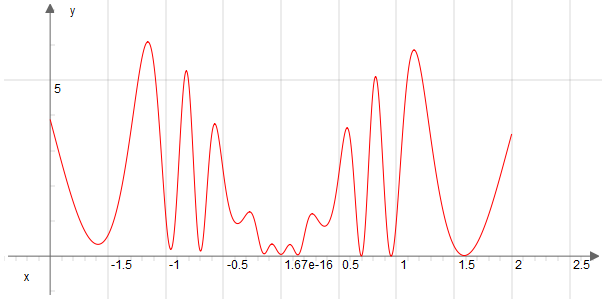
\includegraphics [scale=1] {MHL_TestFunction_Multiextremal}
  \caption{Функция Multiextremal} 
  \label{TestFunctions:img:MHL_TestFunction_Multiextremale}  
\end{figure}

\subsection {Параметры для алгоритмов оптимизации}

\begin{tabularwide}
\textbf{Точность вычислений:} & $\varepsilon=0.01$. \\
\textbf{Число интервалов, на которые предполагается разбивать каждую компоненту вектора $\bar{x}$ в пределах своего изменения} (для алгоритмов дискретной оптимизации) : & $NumberOfParts_j=4095$ ($j=\overline{1,n}$). \\
\textbf{Для этого длина бинарной строки для $x_j$ координаты равна} (для алгоритмов бинарной оптимизации) : & $\left( k_2\right)_j=12$ ($j=\overline{1,n}$). \\
\end{tabularwide}

\textbf{Замечание:}  $NumberOfParts_j$ выбирается как минимальное число, удовлетворяющее соотношению:
\begin{equation*}
NumberOfParts_j=2^{\left( k_2\right)_j }-1\geq\dfrac{10\left( Right_j-Left_j\right) }{\varepsilon},\text{где } \left( k_2\right)_j \in \mathbb{N}, \left( j=\overline{1,n}\right).
\end{equation*}

\subsection {Основная задача и подзадачи}

\begin{tabularwide}
\textbf{Изменяемый параметр: } & $n$ --- размерность вещественного вектора. \\
\textbf{Значение в основной задаче:} & $n=1$.\\
\end{tabularwide}

\subsection {Нахождение ошибки оптимизации}

Пусть в результате работы алгоритма оптимизации за $N$ запусков мы нашли решения $\bar{x}_{submin}^k$ со значениями целевой функции $f\left( \bar{x}_{submin}^k\right) $ соответственно ($k=\overline{1,N}$). Используем три вида ошибок:

\textbf{Надёжность: }
\begin{equation*}
R = \dfrac{\sum_{k=1}^{N}S\left( \bar{x}_{submin}^k \right) }{N}, \text{ где}
\end{equation*}
\begin{equation*}
S\left( \bar{x}_{submin}^k \right)=\left\lbrace \begin{aligned} 1,& \text{ если } \left| \left( \bar{x}_{submin}^k \right)_j-\left( \bar{x}_{min} \right)_j\right|\leq\varepsilon, j=\overline{1,n};   \\ 0,& \text{ иначе}. \end{aligned}\right.
\end{equation*}

\textbf{Ошибка по входным параметрам:}
\begin{equation*}
E_x = \dfrac{\sum_{k=1}^{N} \left( \frac{\sqrt{\sum_{j=1}^{n}{\left( \left( \bar{x}_{submin}^k \right)_j-\left( \bar{x}_{min} \right)_j \right)}^2 }}{n} \right)  }{N}.
\end{equation*}

\textbf{Ошибка по значениям целевой функции: }
\begin{equation*}
E_f = \dfrac{\sum_{k=1}^{N} \left| f\left( \bar{x}_{submin}^k \right)-f\left( \bar{x}_{min} \right) \right|  }{N}.
\end{equation*}

\subsection {Свойства задачи}
\begin{tabularwide}
\textbf{Условной или безусловной оптимизации: } & Задача безусловной оптимизации. \\
\textbf{Одномерной или многомерной оптимизации: } & Одномерной. \\
\textbf{Функция унимодальная или многоэкстремальная: } & Функция многоэкстремальная. \\
\textbf{Функция стохастическая или нет: } & Функция не стохастическая. \\
\textbf{Особенности: } & Нет. \\
\end{tabularwide}

\subsection {Реализация}

Реализация функции взята из библиотеки HarrixMathLibrary в разделе <<Тестовые функции для оптимизации>>, которую можно найти по адресу \href{https://github.com/Harrix/HarrixMathLibrary} {https://github.com/Harrix/HarrixMathLibrary}.

\begin{lstlisting}[caption=Код функции MHL\_TestFunction\_Multiextremal]
double MHL_TestFunction_Multiextremal(double x)
{
/*
Функция одной переменных: функция Multiextremal.
Тестовая функция вещественной оптимизации.
Входные параметры:
 x - вещественная переменная.
Возвращаемое значение:
 Значение тестовой функции в точке (x).
*/
double VMHL_Result;
VMHL_Result = (0.05*(x-1.)*(x-1.)+(3.-2.9*exp(-2.77257*x*x))*(1-cos(x*(4.-50*exp(-2.77257*x*x)))));
return VMHL_Result;
}
\end{lstlisting}

\subsection {Ссылки}

Данная функция приводится в следующих источниках:

\begin{enumerate}
\item \cite[стр. 26]{book:Semenkin2007} ---  \href{http://files.lib.sfu-kras.ru/ebibl/umkd/22/u_lectures.pdf}{Эволюционные методы моделирования и оптимизации сложных систем}.
\end{enumerate}

По сравнению с данной работой в данном документе представлено уточненное значение функции в точке минимума.
\section {Функция Multiextremal2}

\subsection {Описание функции}

\begin{tabularwide}
\textbf{Идентификатор:} & MHL\_TestFunction\_Multiextremal2. \\
\textbf{Наименование:} & Multiextremal2. \\
\textbf{Тип:} & Задача вещественной оптимизации. \\
\end{tabularwide}

\textbf{Формула} (целевая функция):
\begin{equation}
\label{TestFunctions:eq:MHL_TestFunction_Multiextremal2}
f\left( \bar{x}\right) =1-0.5\cos\left( 1.5\left( 10x-0.3\right) \right)\cos\left( 31.4x\right)+0.5\cos\left(\sqrt{5}\cdot10x \right)\cos\left( 35x\right) , \text{ где}  
\end{equation}
\indent $\bar{x}\in X$, $\bar{x}_j\in \left[ Left_j; Right_j\right] $, $Left_j=-2$, $Right_j=2$, $j=\overline{1,n}$, $n=1$.

\begin{tabularwide}
\textbf{Обозначение:} &\specialcell{$\bar{x}$ --- вещественный вектор;\\$n = 1$ --- размерность вещественного вектора.}  \\
\textbf{Решаемая задача оптимизации:} & $\bar{x}_{max}= \arg \max_{\bar{x}\in X} f\left( \bar{x}\right)$.   \\
\textbf{Точка максимума:} & $\bar{x}_{max}\approx{\left( -0.993263\right)}^\mathrm{T} $, то есть $\left(\bar{x}_{max} \right)_j\approx-0.993263$ ($j=\overline{1,n}$).    \\
\textbf{Максимум функции:} & $f\left(\bar{x}_{max} \right) \approx 1.93374$.   \\
\textbf{График:} & Рисунок \ref{TestFunctions:img:MHL_TestFunction_Multiextremal2e} нас \pageref{TestFunctions:img:MHL_TestFunction_Multiextremal2e} стр.   \\
\end{tabularwide}

\begin{figure} [h] 
  \center
  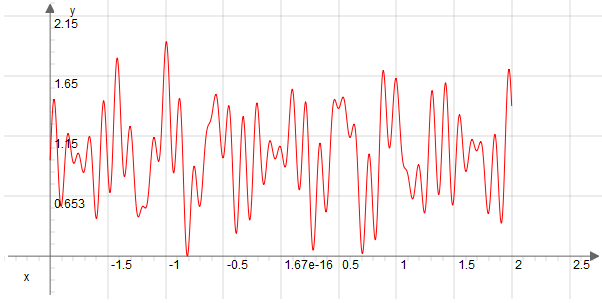
\includegraphics [scale=1] {MHL_TestFunction_Multiextremal2}
  \caption{Функция Multiextremal2} 
  \label{TestFunctions:img:MHL_TestFunction_Multiextremal2e}  
\end{figure}

\subsection {Параметры для алгоритмов оптимизации}

\begin{tabularwide}
\textbf{Точность вычислений:} & $\varepsilon=0.01$. \\
\textbf{Число интервалов, на которые предполагается разбивать каждую компоненту вектора $\bar{x}$ в пределах своего изменения} (для алгоритмов дискретной оптимизации) : & $NumberOfParts_j=4095$ ($j=\overline{1,n}$). \\
\textbf{Для этого длина бинарной строки для $x_j$ координаты равна} (для алгоритмов бинарной оптимизации) : & $\left( k_2\right)_j=12$ ($j=\overline{1,n}$). \\
\end{tabularwide}

\textbf{Замечание:}  $NumberOfParts_j$ выбирается как минимальное число, удовлетворяющее соотношению:
\begin{equation*}
NumberOfParts_j=2^{\left( k_2\right)_j }-1\geq\dfrac{10\left( Right_j-Left_j\right) }{\varepsilon},\text{где } \left( k_2\right)_j \in \mathbb{N}, \left( j=\overline{1,n}\right).
\end{equation*}

\subsection {Основная задача и подзадачи}

\begin{tabularwide}
\textbf{Изменяемый параметр: } & $n$ --- размерность вещественного вектора. \\
\textbf{Значение в основной задаче:} & $n=1$.\\
\end{tabularwide}

\subsection {Нахождение ошибки оптимизации}

Пусть в результате работы алгоритма оптимизации за $N$ запусков мы нашли решения $\bar{x}_{submin}^k$ со значениями целевой функции $f\left( \bar{x}_{submin}^k\right) $ соответственно ($k=\overline{1,N}$). Используем три вида ошибок:

\textbf{Надёжность: }
\begin{equation*}
R = \dfrac{\sum_{k=1}^{N}S\left( \bar{x}_{submin}^k \right) }{N}, \text{ где}
\end{equation*}
\begin{equation*}
S\left( \bar{x}_{submin}^k \right)=\left\lbrace \begin{aligned} 1,& \text{ если } \left| \left( \bar{x}_{submin}^k \right)_j-\left( \bar{x}_{min} \right)_j\right|<\varepsilon, j=\overline{1,n};   \\ 0,& \text{ иначе}. \end{aligned}\right.
\end{equation*}

\textbf{Ошибка по входным параметрам:}
\begin{equation*}
E_x = \dfrac{\sum_{k=1}^{N} \left( \frac{\sqrt{\sum_{j=1}^{n}{\left( \left( \bar{x}_{submin}^k \right)_j-\left( \bar{x}_{min} \right)_j \right)}^2 }}{n} \right)  }{N}.
\end{equation*}

\textbf{Ошибка по значениям целевой функции: }
\begin{equation*}
E_f = \dfrac{\sum_{k=1}^{N} \left| f\left( \bar{x}_{submin}^k \right)-f\left( \bar{x}_{min} \right) \right|  }{N}.
\end{equation*}

\subsection {Свойства задачи}
\begin{tabularwide}
\textbf{Условной или безусловной оптимизации: } & Задача безусловной оптимизации. \\
\textbf{Одномерной или многомерной оптимизации: } & Одномерной. \\
\textbf{Функция унимодальная или многоэкстремальная: } & Функция многоэкстремальная. \\
\textbf{Функция стохастическая или нет: } & Функция не стохастическая. \\
\textbf{Особенности: } & Нет. \\
\end{tabularwide}

\subsection {Реализация}

Реализация функции взята из библиотеки HarrixMathLibrary в разделе <<Тестовые функции для оптимизации>>, которую можно найти по адресу \href{https://github.com/Harrix/HarrixMathLibrary} {https://github.com/Harrix/HarrixMathLibrary}.

\begin{lstlisting}[caption=Код функции MHL\_TestFunction\_Multiextremal2]
double MHL_TestFunction_Multiextremal2(double x)
{
/*
Функция одной переменных: функция Multiextremal2.
Тестовая функция вещественной оптимизации.
Входные параметры:
 x - вещественная переменная.
Возвращаемое значение:
 Значение тестовой функции в точке (x).
*/
double VMHL_Result;
VMHL_Result = 1.-0.5*cos(1.5*(10.*x-0.3))*cos(31.4*x)+0.5*cos(sqrt(5.)*10.*x)*cos(35.*x);
return VMHL_Result;
}
\end{lstlisting}

\subsection {Ссылки}

Данная функция приводится в следующих источниках:

\begin{enumerate}
\item \cite[стр. 27]{book:Semenkin2007} ---  \href{http://files.lib.sfu-kras.ru/ebibl/umkd/22/u_lectures.pdf}{Эволюционные методы моделирования и оптимизации сложных систем}.
\end{enumerate}

По сравнению с данной работой в данном документе представлено уточненное значение функции в точке минимума.
\section {Функция волна}

\subsection {Описание функции}

\begin{tabularwide}
\textbf{Идентификатор:} & MHL\_TestFunction\_Wave. \\
\textbf{Наименование:} & Волна. \\
\textbf{Тип:} & Задача вещественной оптимизации. \\
\end{tabularwide}

\textbf{Формула} (целевая функция):
\begin{equation}
\label{TestFunctions:eq:MHL_TestFunction_Wave}
f\left( \bar{x}\right) = e^{ -\bar{x}_1^2}+0.01\cos\left( 200\cdot\bar{x}_1\right)    , \text{ где}
\end{equation}
\indent $\bar{x}\in X$, $\bar{x}_j\in \left[ Left_j; Right_j\right] $, $Left_j=-2$, $Right_j=2$, $j=\overline{1,n}$, $n=1$.

\begin{tabularwide}
\textbf{Обозначение:} &\specialcell{$\bar{x}$ --- вещественный вектор;\\$n = 1$ --- размерность вещественного вектора.}  \\
\textbf{Решаемая задача оптимизации:} & $\bar{x}_{max}= \arg \max_{\bar{x}\in X} f\left( \bar{x}\right)$.   \\
\textbf{Точка максимума:} & $\bar{x}_{max}={\left( 0\right)}^\mathrm{T} $, то есть $\left(\bar{x}_{max} \right)_j=0$ ($j=\overline{1,n}$).    \\
\textbf{Максимум функции:} & $f\left(\bar{x}_{max} \right) =1.01$.   \\
\textbf{График:} & Рисунок \ref{TestFunctions:img:MHL_TestFunction_Wavee} нас \pageref{TestFunctions:img:MHL_TestFunction_Wavee} стр.   \\
\end{tabularwide}

\begin{figure} [h] 
  \center
  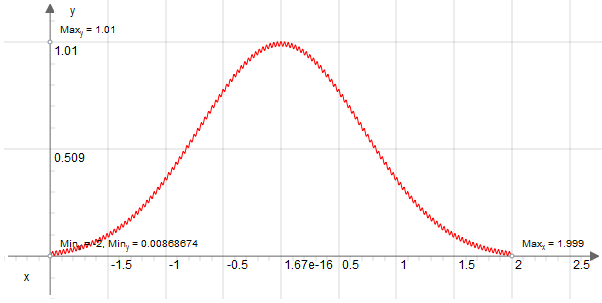
\includegraphics [scale=1] {MHL_TestFunction_Wave}
  \caption{Волна} 
  \label{TestFunctions:img:MHL_TestFunction_Wavee}  
\end{figure}

\subsection {Параметры для алгоритмов оптимизации}

\begin{tabularwide}
\textbf{Точность вычислений:} & $\varepsilon=0.01$. \\
\textbf{Число интервалов, на которые предполагается разбивать каждую компоненту вектора $\bar{x}$ в пределах своего изменения} (для алгоритмов дискретной оптимизации) : & $NumberOfParts_j=4095$ ($j=\overline{1,n}$). \\
\textbf{Для этого длина бинарной строки для $x_j$ координаты равна} (для алгоритмов бинарной оптимизации) : & $\left( k_2\right)_j=12$ ($j=\overline{1,n}$). \\
\end{tabularwide}

\textbf{Замечание:}  $NumberOfParts_j$ выбирается как минимальное число, удовлетворяющее соотношению:
\begin{equation*}
NumberOfParts_j=2^{\left( k_2\right)_j }-1\geq\dfrac{10\left( Right_j-Left_j\right) }{\varepsilon},\text{где } \left( k_2\right)_j \in \mathbb{N}, \left( j=\overline{1,n}\right).
\end{equation*}

\subsection {Основная задача и подзадачи}

\begin{tabularwide}
\textbf{Изменяемый параметр: } & $n$ --- размерность вещественного вектора. \\
\textbf{Значение в основной задаче:} & $n=1$.\\
\end{tabularwide}

\subsection {Нахождение ошибки оптимизации}

Пусть в результате работы алгоритма оптимизации за $N$ запусков мы нашли решения $\bar{x}_{submin}^k$ со значениями целевой функции $f\left( \bar{x}_{submin}^k\right) $ соответственно ($k=\overline{1,N}$). Используем три вида ошибок:

\textbf{Надёжность: }
\begin{equation*}
R = \dfrac{\sum_{k=1}^{N}S\left( \bar{x}_{submin}^k \right) }{N}, \text{ где}
\end{equation*}
\begin{equation*}
S\left( \bar{x}_{submin}^k \right)=\left\lbrace \begin{aligned} 1,& \text{ если } \left| \left( \bar{x}_{submin}^k \right)_j-\left( \bar{x}_{min} \right)_j\right|<\varepsilon, j=\overline{1,n};   \\ 0,& \text{ иначе}. \end{aligned}\right.
\end{equation*}

\textbf{Ошибка по входным параметрам:}
\begin{equation*}
E_x = \dfrac{\sum_{k=1}^{N} \left( \frac{\sqrt{\sum_{j=1}^{n}{\left( \left( \bar{x}_{submin}^k \right)_j-\left( \bar{x}_{min} \right)_j \right)}^2 }}{n} \right)  }{N}.
\end{equation*}

\textbf{Ошибка по значениям целевой функции: }
\begin{equation*}
E_f = \dfrac{\sum_{k=1}^{N} \left| f\left( \bar{x}_{submin}^k \right)-f\left( \bar{x}_{min} \right) \right|  }{N}.
\end{equation*}

\subsection {Свойства задачи}
\begin{tabularwide}
\textbf{Условной или безусловной оптимизации: } & Задача безусловной оптимизации. \\
\textbf{Одномерной или многомерной оптимизации: } & Одномерной. \\
\textbf{Функция унимодальная или многоэкстремальная: } & Функция многоэкстремальная. \\
\textbf{Функция стохастическая или нет: } & Функция не стохастическая. \\
\textbf{Особенности: } & Хотя внешне можно отнести эту функцию к стохастической, так как по поведению напоминает вид плотности нормального распределения с помехой. \\
\end{tabularwide}

\subsection {Реализация}

Реализация функции взята из библиотеки HarrixMathLibrary в разделе <<Тестовые функции для оптимизации>>, которую можно найти по адресу \href{https://github.com/Harrix/HarrixMathLibrary} {https://github.com/Harrix/HarrixMathLibrary}.

\begin{lstlisting}[caption=Код функции MHL\_TestFunction\_Wave]
double MHL_TestFunction_Wave(double x)
{
/*
Функция одной переменных: волна.
Тестовая функция вещественной оптимизации.
Входные параметры:
 x - вещественная переменная.
Возвращаемое значение:
 Значение тестовой функции в точке (x).
*/
double VMHL_Result;
VMHL_Result = (exp(-x*x)+0.01*cos(200*x));
return VMHL_Result;
}
\end{lstlisting}

\subsection {Ссылки}

Так и не смог найти нормальный источник для этой функции. Откуда-то у меня находится со студенческих времен.
\clearpage


\chapter{Задачи бинарной оптимизации}
\section {Сумма всех элементов бинарного вектора}
\label{TestFunctions:section:MHL_TestFunction_SumVector}
\subsection {Описание функции}

\begin{tabularwide}
\textbf{Идентификатор:} & MHL\_TestFunction\_SumVector. \\
\textbf{Наименование:} & Сумма всех элементов бинарного вектора. \\
\textbf{Тип:} & Задача бинарной оптимизации. \\
\end{tabularwide}

\textbf{Формула} (целевая функция):
\begin{equation}
\label{TestFunctions:eq:MHL_TestFunction_SumVector}
f\left( \bar{x}\right) = \sum_{i=1}^{n}\bar{x}_i, \text{ где}
\end{equation}
\indent $\bar{x}\in X$, $\bar{x}_j\in \left\lbrace 0; 1 \right\rbrace  $, $j=\overline{1,n}$.

\begin{tabularwide}
\textbf{Обозначение:} &\specialcell{$\bar{x}$ --- бинарный вектор;\\$n$ --- размерность бинарного вектора.}  \\
\textbf{Объем поискового пространства:} & $\mu\left( X\right)=2^n $.   \\
\textbf{Решаемая задача оптимизации:} & $\bar{x}_{max}= \arg \max_{\bar{x}\in X} f\left( \bar{x}\right)$.   \\
\textbf{Точка максимума:} & $\bar{x}_{max}={\left( 1,1,\ldots,1\right)}^\mathrm{T} $, то есть $\left(\bar{x}_{max} \right)_j=1$ ($j=\overline{1,n}$).    \\
\textbf{Максимум функции:} & $f\left(\bar{x}_{max} \right) =n$.   \\
\textbf{Точка минимума:} & $\bar{x}_{min}={\left( 0,0,\ldots,0\right)}^\mathrm{T} $, то есть $\left(\bar{x}_{min} \right)_j=0$ ($j=\overline{1,n}$).    \\
\textbf{Минимум функции:} & $f\left(\bar{x}_{min} \right) =0$.   \\
\end{tabularwide}

\subsection {Основная задача и подзадачи}

\begin{tabularwide}
\textbf{Изменяемый параметр: } & $n$ --- размерность бинарного вектора. \\
\textbf{Значение в основной задаче:} & $n=20$.\\
\textbf{Подзадача №2:} & $n=30$.\\
\textbf{Подзадача №3:} & $n=40$.\\
\textbf{Подзадача №4:} & $n=50$.\\
\textbf{Подзадача №5:} & $n=60$.\\
\textbf{Подзадача №6:} & $n=70$.\\
\textbf{Подзадача №7:} & $n=80$.\\
\textbf{Подзадача №8:} & $n=90$.\\
\textbf{Подзадача №9:} & $n=100$.\\
\textbf{Подзадача №10:} & $n=200$.\\
\end{tabularwide}

\subsection {Нахождение ошибки оптимизации}

Пусть в результате работы алгоритма оптимизации за $N$ запусков мы нашли решения $\bar{x}_{submax}^k$ со значениями целевой функции $f\left( \bar{x}_{submax}^k\right) $ соответственно ($k=\overline{1,N}$). Используем три вида ошибок:

\textbf{Надёжность: }
\begin{equation*}
R = \dfrac{\sum_{k=1}^{N}S\left( \bar{x}_{submax}^k \right) }{N}, \text{ где}
\end{equation*}
\begin{equation*}
S\left( \bar{x}_{submax}^k \right)=\left\lbrace \begin{aligned} 1,& \text{ если } \bar{x}_{submax}^k = \bar{x}_{max} ;   \\ 0,& \text{ иначе}. \end{aligned}\right.
\end{equation*}

\textbf{Ошибка по входным параметрам:}
\begin{equation*}
E_x = \dfrac{\sum_{k=1}^{N} \left( \frac{\sum_{j=1}^{n}\left| \left( \bar{x}_{submax}^k \right)_j-\left( \bar{x}_{max} \right)_j \right| }{n} \right)  }{N}.
\end{equation*}

\textbf{Ошибка по значениям целевой функции: }
\begin{equation*}
E_f = \dfrac{\sum_{k=1}^{N} \left( \frac{\left| f\left( \bar{x}_{submax}^k \right)-f\left( \bar{x}_{max} \right) \right|}{n}\right)   }{N}.
\end{equation*}

\subsection {Свойства задачи}
\begin{tabularwide}
\textbf{Условной или безусловной оптимизации: } & Задача безусловной оптимизации. \\
\textbf{Одномерной или многомерной оптимизации: } & Многомерной: $ n $. \\
\textbf{Функция унимодальная или многоэкстремальная: } & Функция унимодальная. \\
\textbf{Функция стохастическая или нет: } & Функция не стохастическая. \\
\textbf{Особенности: } & Нет. \\
\end{tabularwide}

\subsection {Реализация}

Реализация функции взята из библиотеки HarrixMathLibrary в разделе <<Тестовые функции для оптимизации>>, которую можно найти по адресу \href{https://github.com/Harrix/HarrixMathLibrary} {https://github.com/Harrix/HarrixMathLibrary}.

\begin{lstlisting}[caption=Код функции MHL\_TestFunction\_SumVector]
double MHL_TestFunction_SumVector(int *x, int VMHL_N)
{
/*
Сумма всех элементов бинарного вектора.
Тестовая функция бинарной оптимизации.
Входные параметры:
 x - указатель на исходный массив;
 VMHL_N - размер массива x.
Возвращаемое значение:
 Значение тестовой функции в точке x.
*/
double VMHL_Result=0;
for (int i=0;i<VMHL_N;i++) VMHL_Result+=x[i];
return VMHL_Result;
}

\end{lstlisting}
\clearpage

% Список литературы
\addcontentsline{toc}{chapter}{\bibname}
\bibliographystyle{utf8gost705u}  %% стилевой файл для оформления по ГОСТу
\bibliography{biblio}     %% имя библиографической базы (bib-файла)

\end{document}
